\documentclass[hyperref=colorlinks]{beamer}
\mode<presentation>
\usetheme{iclpt}
\setbeamertemplate{navigation symbols}{}
\setbeamertemplate{headline}{
\begin{beamercolorbox}[leftskip=.2cm,rightskip=.2cm,topskip=.2cm,ht=1.1cm,dp=0.1cm,wd=\textwidth]{institute in head/foot}
  
\includegraphics[height=1cm]{icl.pdf}
  \hfill
  
\includegraphics[height=1cm]{../Pics/CMS-Color.pdf}
\end{beamercolorbox}
}
\setbeamertemplate{footline}{
\begin{beamercolorbox}[ht=.55cm,dp=0.4cm,wd=\textwidth,leftskip=.3cm]{author in head/foot}%
  \begin{minipage}[c]{5cm}%
    \usebeamerfont{author in head/foot}
    \insertshortauthor 
    \insertshorttitle
    \end{minipage}\hfill%
  \insertframenumber{} / \pageref{lastframe}
  \hfill
  \begin{minipage}{6cm}
    \hfill
  \end{minipage}
\end{beamercolorbox}%
}

\usepackage{color}
\usepackage{tabularx,colortbl}
\usepackage{graphicx}
\usepackage{pdfpages}
\usepackage{feynmp}
\usepackage{multirow}
\DeclareGraphicsRule{*}{mps}{*}{}

\title{\vspace{-0.2cm} VBF Higgs to Invisible - Towards Run II}
\subtitle{HIG-14-038, AN-14-243\vspace{-0.7cm}}
\author[P. Dunne]{C. Asawatangtrakuldee, J. Brooke, D. Colling, G. Davies, \underline{P. Dunne}, A.M. Magnan, A. Nikitenko, J. Pela}
\titlegraphic{
  \vspace{-0.7cm}
  %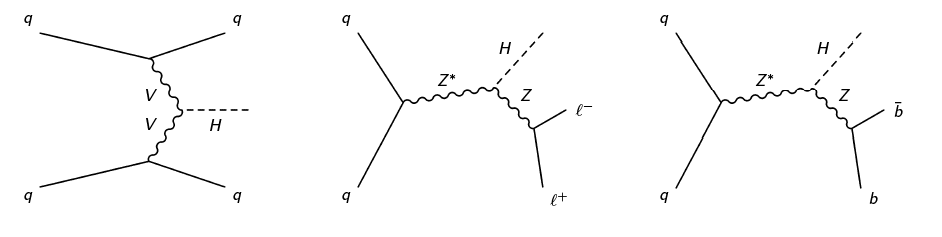
\includegraphics[width=\textwidth]{TalkPics/invcomb021213/feyndiags}
%% \begin{fmfgraph*}(100,70)
%%         \fmfleft{i1,i2}
%%         \fmfright{o1,o2,o3}
%%         \fmf{fermion}{i1,v1,o1}
%%         \fmf{fermion}{i2,v2,o3}
%%         \fmf{phantom,tension=4/5}{v1,v2}
%%         \fmffreeze
%%         \fmf{photon,label=$W,,Z$}{v1,v3}
%%         \fmf{photon,label=$W,,Z$}{v2,v3}
%%         \fmf{dashes}{v3,o2}
%%         \fmflabel{$q$}{i1}
%%         \fmflabel{$q$}{i2}
%%         \fmflabel{$q$}{o1}
%%         \fmflabel{$q$}{o3}
%%         \fmflabel{$H$}{o2}
%%       \end{fmfgraph*}
}
\date{}
\begin{document}
\begin{fmffile}{hig14038preapprovalfeyndiags}

%TITLE PAGE
\section{Title}
\begin{frame}
  \titlepage
  
\end{frame}

%!!CLOSURE TEST STATEMENT PU jet ID

%OUTLINE
\begin{frame}
  \begin{columns}
    \column{.65\textwidth}
    \begin{block}{\footnotesize Reminder}
      \scriptsize
      \begin{itemize}
      \item Motivation is the same as run 1:
      \item[-] Complemented by direct DM and indirect B(H$\rightarrow$ inv) searches
      \item For Run 1 we had two sets of triggers
      \item[-] Prompt trigger used for published result: HIG-13-30
      \item[-] Parked triggers: analysis presented today
      \item[-] Parked analysis will be used as baseline for run 2
      \end{itemize}
    \end{block}
    \begin{block}{\footnotesize Overview}
      \scriptsize
      \begin{itemize}
      \item Reminder of prompt analysis
      \item Details of parked analysis
      \item[-] Emphasis on changes from established prompt analysis
      \item Trigger plans for run 2
      \end{itemize}
    \end{block}
    \column{.45\textwidth}
    \vspace{0.7cm}

    \begin{fmfgraph*}(100,70)                                                                                                                              
        \fmfleft{i1,i2}                                                                                                                                   
        \fmfright{o1,o2,o3}                                                                                                                               
        \fmf{fermion}{i1,v1,o1}                                                                                                                           
        \fmf{fermion}{i2,v2,o3}                                                                                                                           
        \fmf{phantom,tension=4/5}{v1,v2}                                                                                                                  
        \fmffreeze                                                                                                                                        
        \fmf{photon,label=$W,,Z$}{v1,v3}                                                                                                                  
        \fmf{photon,label=$W,,Z$}{v2,v3}                                                                                                                  
        \fmf{dashes}{v3,o2}                                                                                                                               
        \fmflabel{$q$}{i1}                                                                                                                                
        \fmflabel{$q$}{i2}                                                                                                                                
        \fmflabel{$q$}{o1}                                                                                                                                
        \fmflabel{$q$}{o3}                                                                                                                                
        \fmflabel{$H$}{o2}                                                                                                                                
      \end{fmfgraph*}

    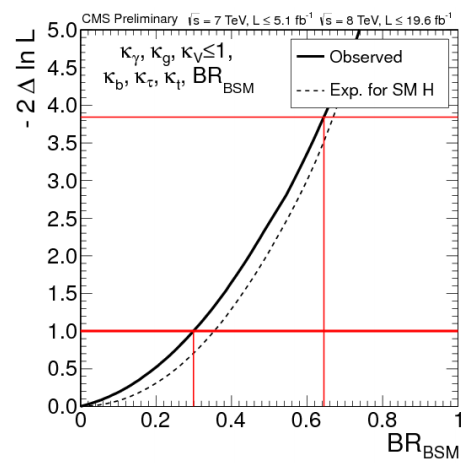
\includegraphics[width=\textwidth,height=.5\textheight]{indirectbrbsm.png}
    \end{columns}
\end{frame}


\begin{frame}
  \frametitle{Prompt Analysis}
  \begin{columns}
    \column{.5\textwidth}
    \vspace{-.4cm}

    \begin{block}{}
      \scriptsize
      \begin{itemize}
      \item Standard object definition:
      \item[-] Details in backup
      \item Single bin counting experiment
      \item[-] Signal region chosen to eliminate QCD and be above trigger turn ons
      \item Major backgrounds use data driven estimates:
      \item[-] $Z\rightarrow\nu\nu$,$W\rightarrow\ell\nu$, QCD
      \item Minor backgrounds taken from MC:
      \item[-] VV, W$\gamma$, $t\bar{t}$, single top
      \item Expected \hspace{-.1cm} limit 49\% at \hspace{-.1cm} $m_{H}=125$ \hspace{-.1cm}GeV
      \end{itemize}
    \end{block}
    \column{.5\textwidth}
    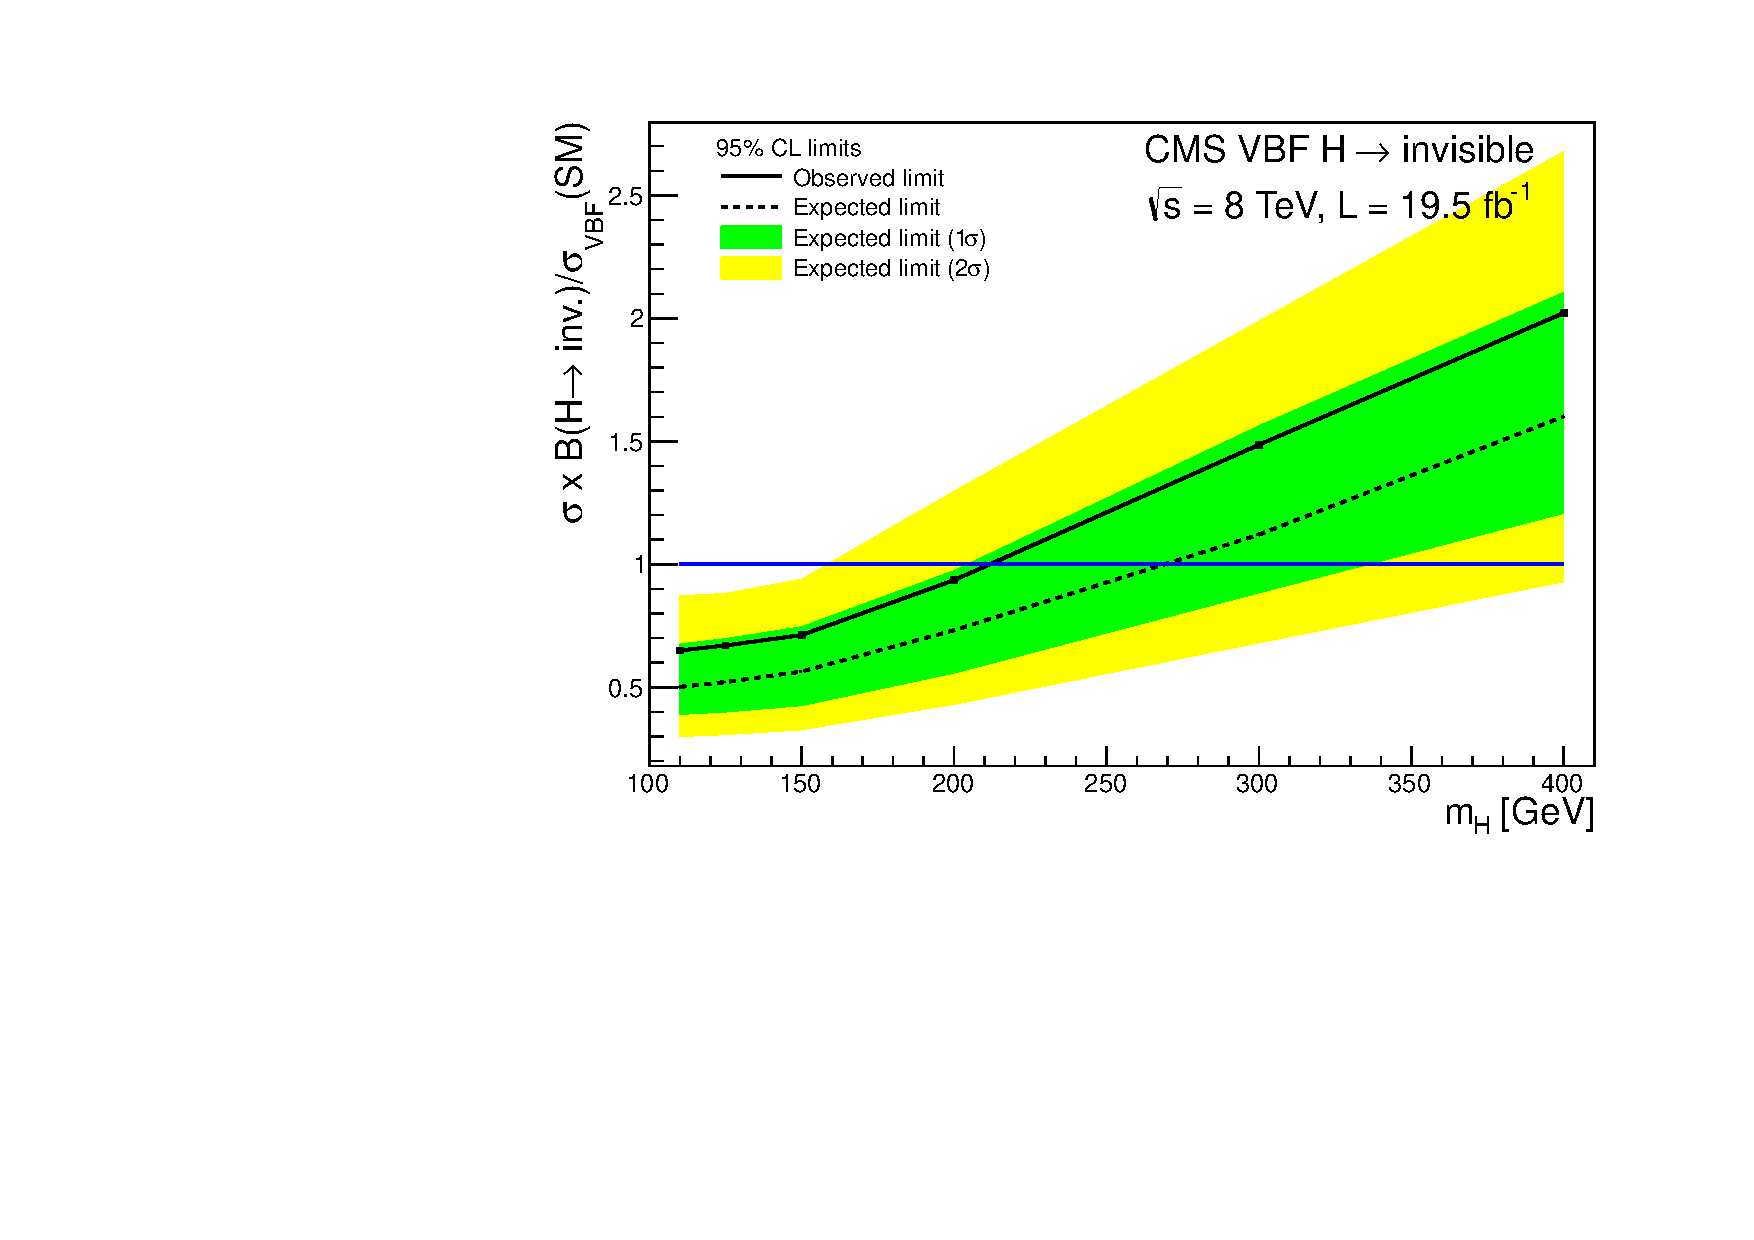
\includegraphics[width=\textwidth]{TalkPics/hig1330approval/vbflimit.pdf}
  \end{columns}
  \vspace{-.2cm}

  \begin{columns}
    \column{1.08\textwidth}
  \begin{block}{\scriptsize Data driven background estimation}
    \begin{columns}
      \column{.35\textwidth}
      \scriptsize
     W: $N_{S}=N_{S}^{MC}\frac{N_{C}^{Data}-N_{C}^{Bkg}}{N_{C}^{MC}}$
     \column{.55\textwidth}
     \scriptsize  
   Z: $N_{S}^{Z\rightarrow\nu\nu}=\left(N_{C}^{Data}-N_{C}^{bkg}\right) \cdot\frac{\sigma\left(Z\rightarrow\nu\nu\right)}{\sigma\left(Z/\gamma^{*}\rightarrow\mu\mu\right)}\cdot \frac{\epsilon_{S}^{ZMC}}{\epsilon_{C}^{ZMC}}$
       \end{columns}
  \end{block}
  \end{columns}
\end{frame}

\begin{frame}
  \frametitle{Parked Analysis}
  \vspace{-.3cm}

  \begin{block}{}
    \scriptsize
    \begin{itemize}
    \item All parked and prompt triggers are seeded by L1\_ETM40
    \item Parked triggers have looser HLT thresholds:
    \item[-] this allows us to look at new phase space regions and analysis techniques
    \item[-] also increases QCD and PU backgrounds
    \end{itemize}
  \end{block}
  \vspace{-.1cm}
  \begin{block}{\scriptsize Trigger Efficiency}
    \scriptsize
    \begin{itemize}
    \item Trigger efficiency has been measured including correlation between variables
    \item[-] This allows the trigger turn on region to be used
    \item[-] Control triggers will be required to do this for run 2
    \end{itemize}
  \end{block}
  \vspace{-.1cm}
  \begin{block}{\scriptsize Signal region}
    \scriptsize
    \begin{itemize}
    \item QCD hard to model, signal region cuts are chosen to make remaining QCD small whilst enhancing real-MET using new Min$\Delta\phi$(jet,MET) variable
    \item The signal region has been reoptimised for the looser parked triggers
    \item[-] New region uses new variable has higher signal efficiency with much less QCD
    \end{itemize}
  \end{block}
  \vspace{-.2cm}
  
\end{frame}


\begin{frame}
  \frametitle{Starting point for region choice}
  \vspace{-.4cm}
  \begin{columns}
    \column{1.05\textwidth}
  \begin{block}{}
    \scriptsize
    \begin{itemize}
    \item Trigger turn ons and detector acceptance impose the following cuts:
    \item[-] $\eta_{j1} \cdot \eta_{j2}<0,\, |\eta_{j1,2}|<4.7,\, \text{jet\,1}\, p_{T}>50 \,\text{GeV},\, \Delta\eta_{jj}>3.6,$\\$\, \text{jet\,2}\, p_{T}>40 \,\text{GeV},\text{METnomu}>90\,\text{GeV},\, M_{jj}>800 \,\text{GeV}$
    \item QCD in plots is VBF enriched MC doesn't model all QCD
    \item Following cuts added due to poor data-MC agreement from QCD contamination:
    \item $\frac{METnomu}{\sigma_{METnomu}}>3.0,\,\text{Min}\Delta\phi(all\,jets\,p_{T}>30\,GeV,METnomu)>1.0,\,M_{jj}>1000\,\text{GeV}$
    \end{itemize}
  \end{block}
  \end{columns}
  \begin{columns}
    \column{1.15\textwidth}
  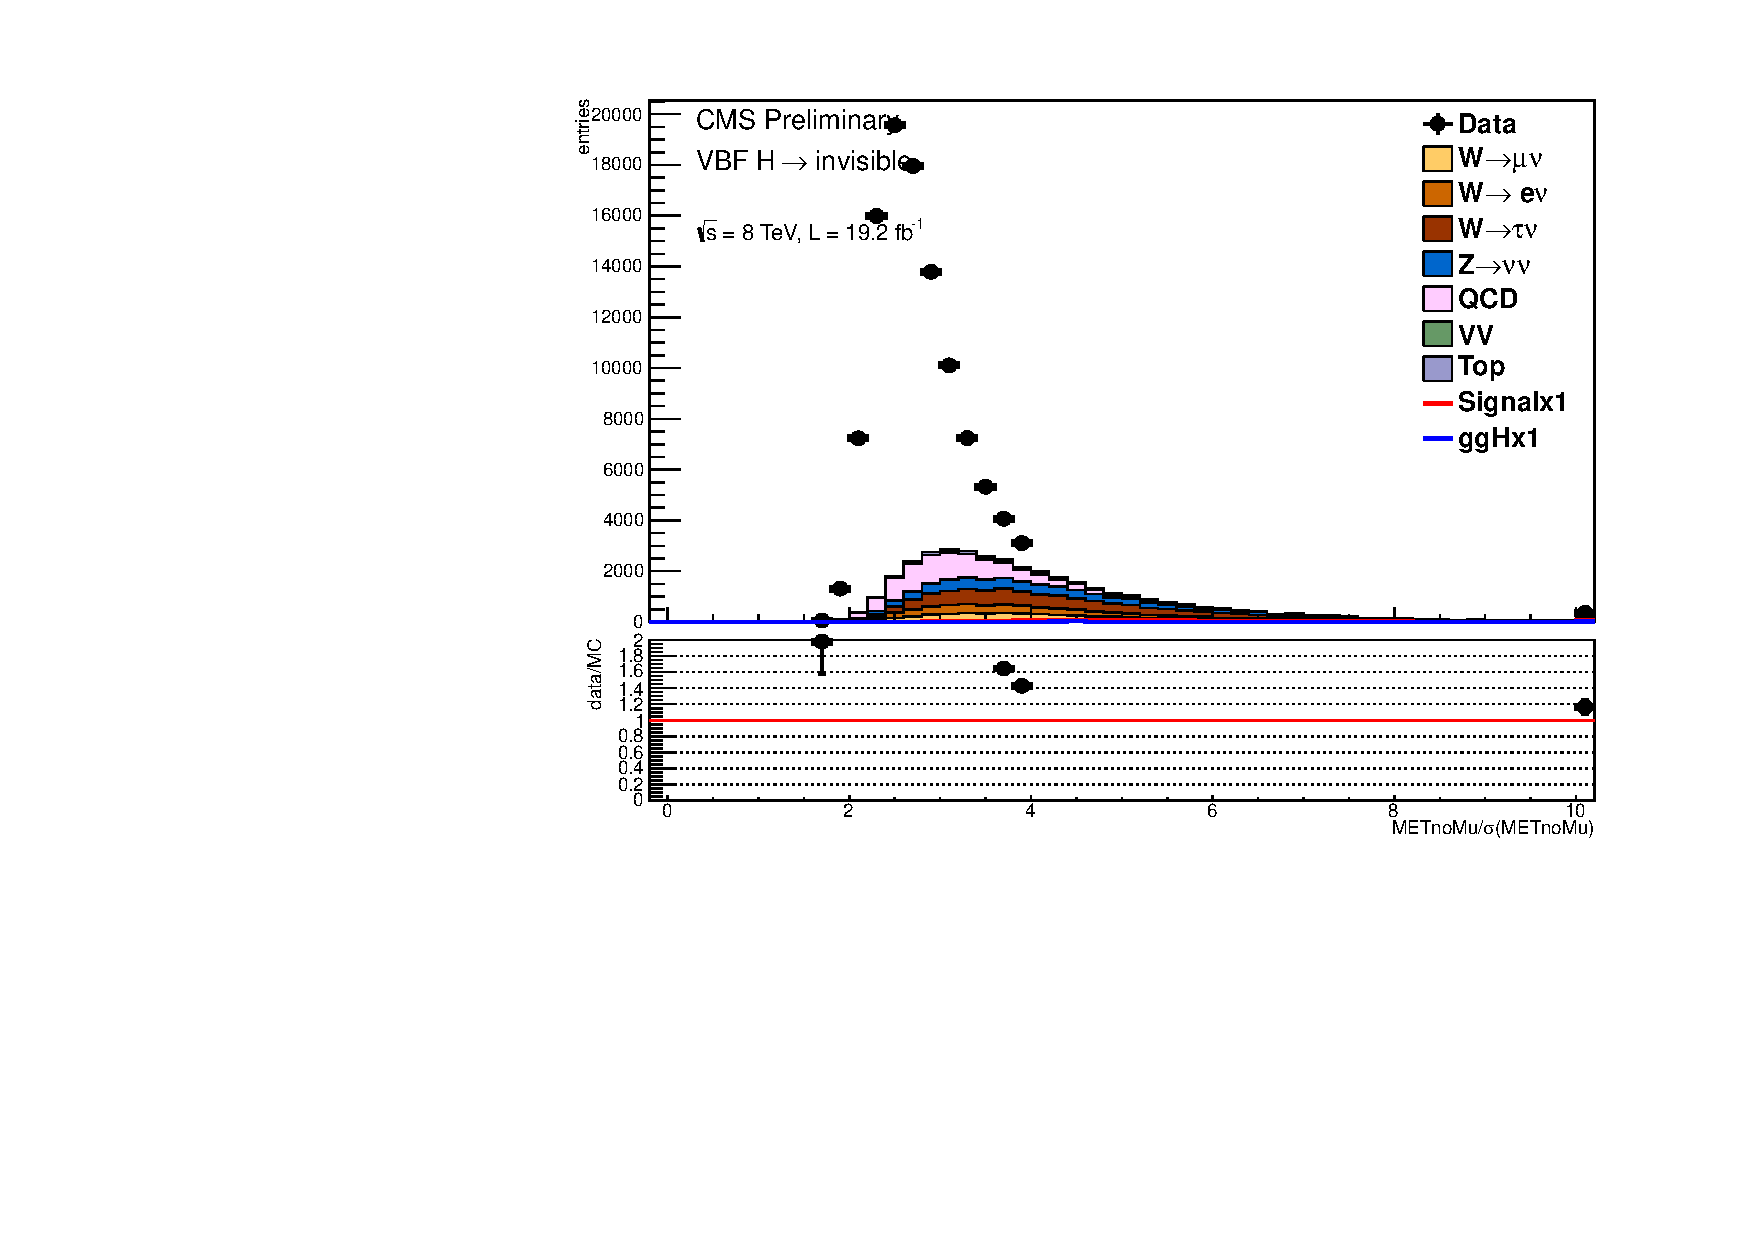
\includegraphics[width=.34\textwidth]{TalkPics/hig14038preapproval/nopreselnunu_metnomu_significance.pdf}
  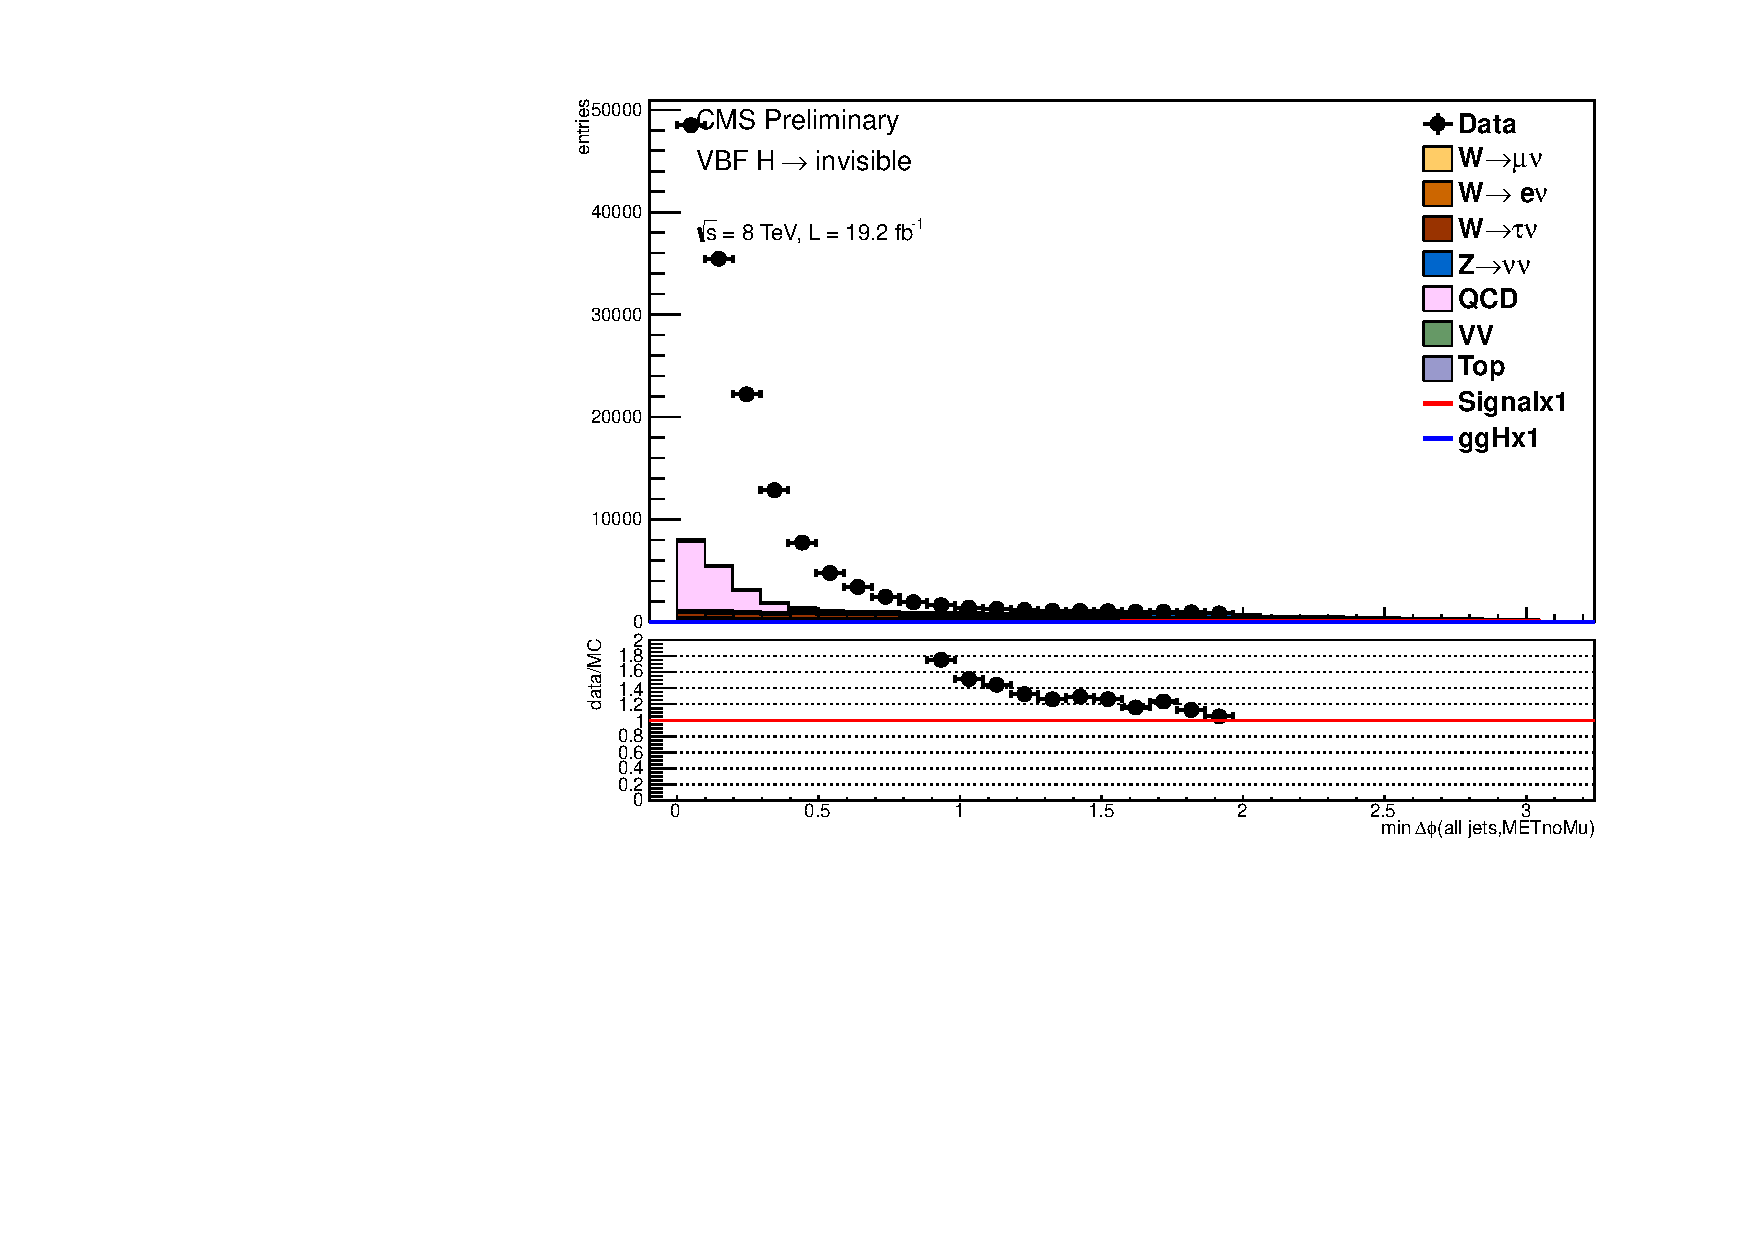
\includegraphics[width=.34\textwidth]{TalkPics/hig14038preapproval/metsigpreselnunu_alljetsmetnomu_mindphi.pdf}
  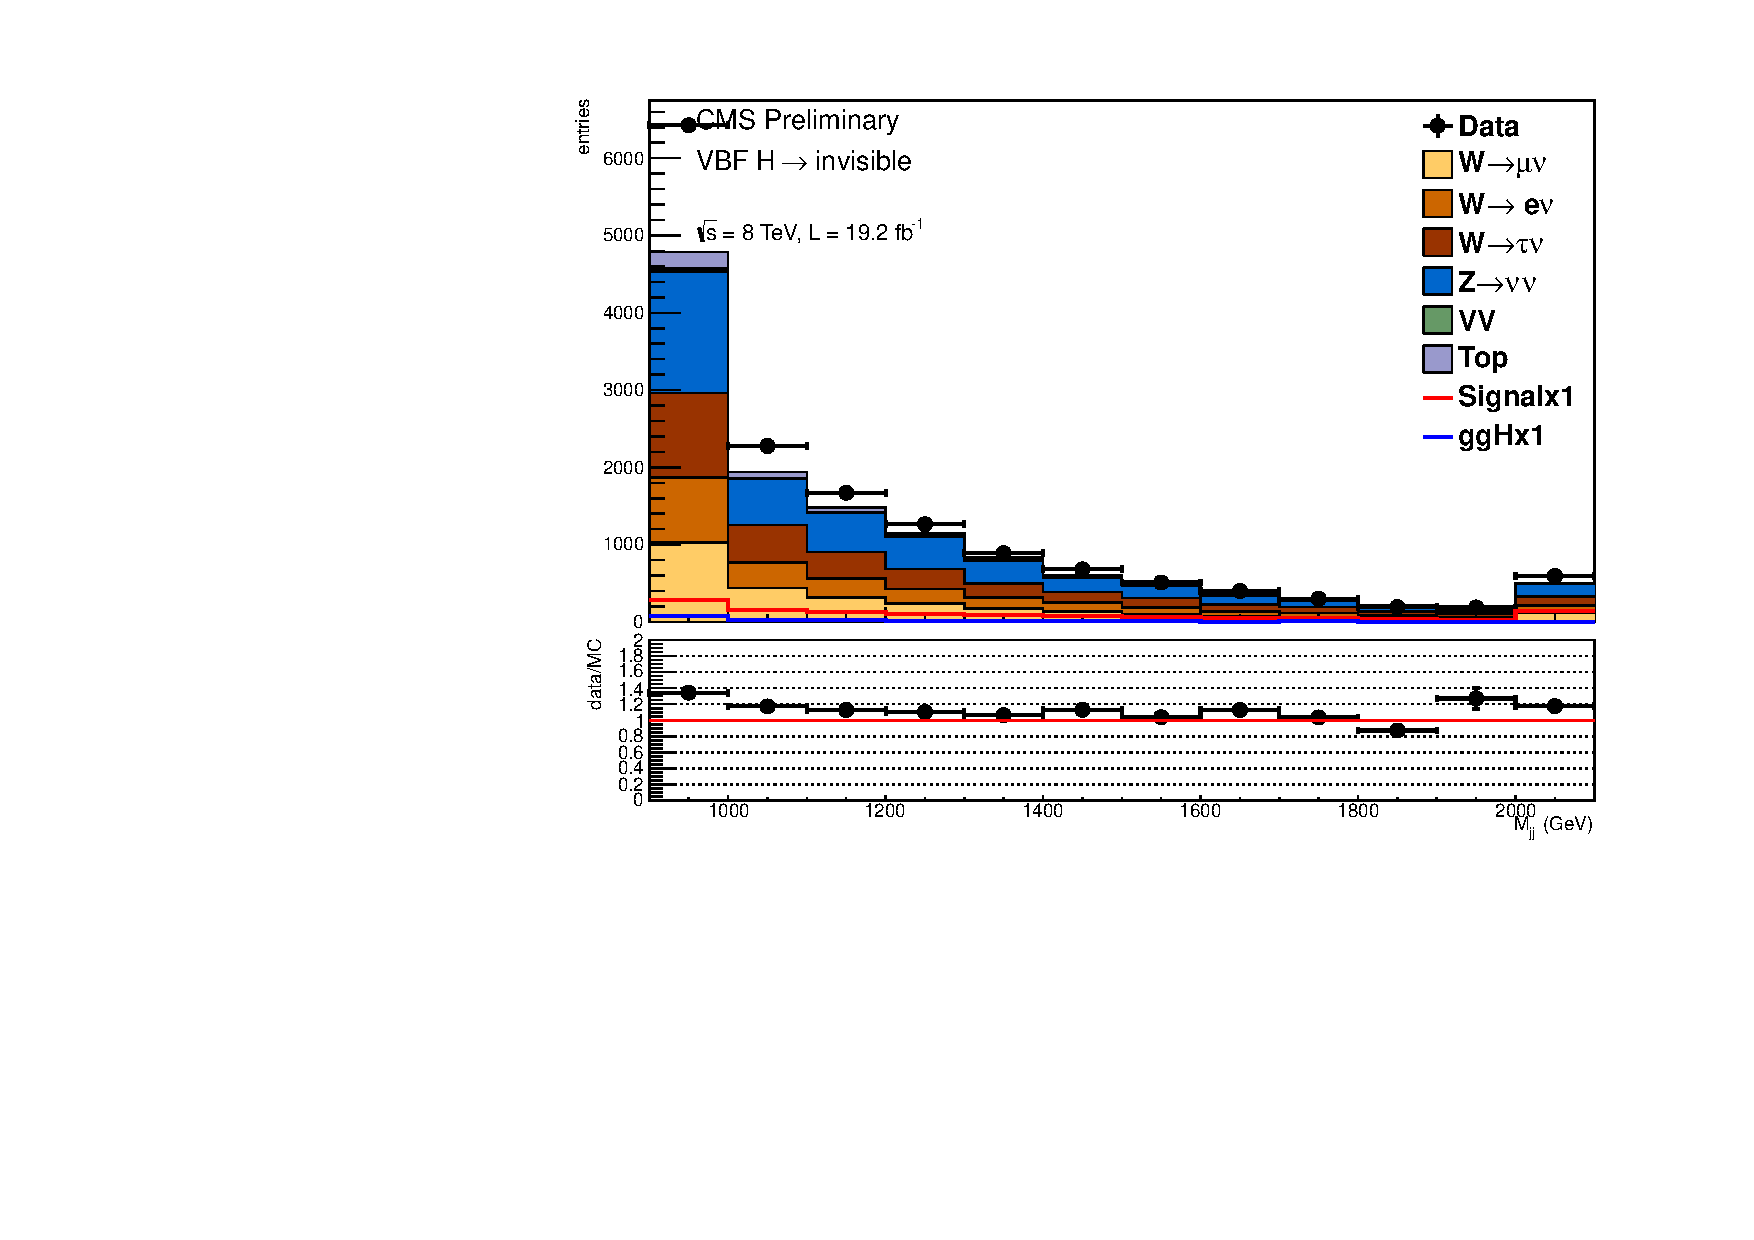
\includegraphics[width=.34\textwidth]{TalkPics/hig14038preapproval/mjj800nunu_dijet_M.pdf}
  \end{columns}
\end{frame}

%SIGNAL SELECTION TAKE AN PLOTS
\begin{frame}
  \frametitle{Signal region selection}
   \begin{columns}
     \column{.55\textwidth}
     \begin{block}{}
       \scriptsize
       \begin{itemize}
       \item As in the prompt analysis we veto events with 'veto' electrons or muons
         \vspace{-.1cm}
       \item Can't model QCD shape so cut hard to remove most QCD
         \vspace{-.1cm}
       \item[-] Can then tolerate a larger uncertainty on QCD estimation
       \item Select region $\frac{METnoMU}{\sigma_{METnoMU}}>4$ and $\text{Min}\Delta\phi(all\,jets,METnomu)>2.0$
       \item Signal contribution also large in this region of parameter space
         \vspace{-.1cm}
       \item[-] We blind this region and use as a basis for signal region optimisation
       \end{itemize}
    \end{block}
    \column{.5\textwidth}
    \vspace{-.25cm}

    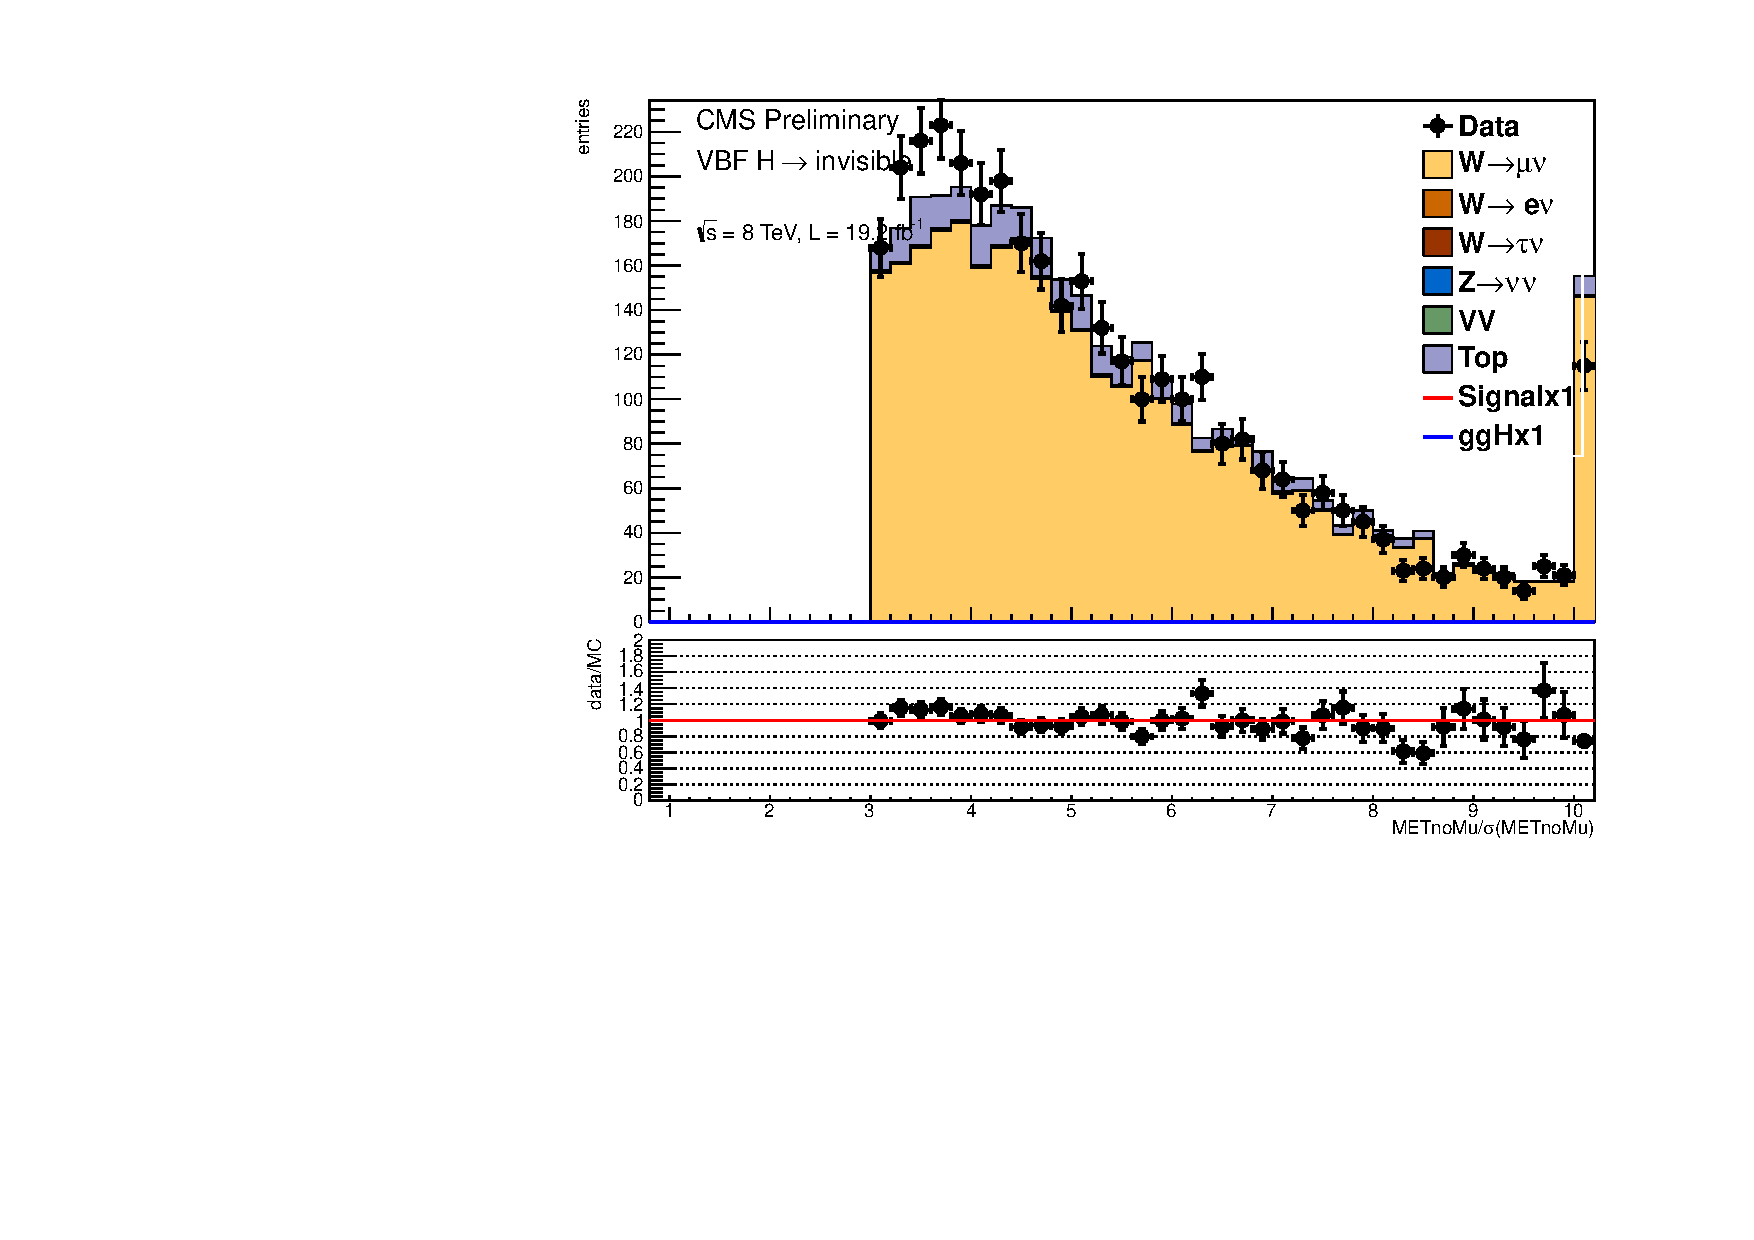
\includegraphics[clip=true,trim=0 0 0 20,width=.95\textwidth]{TalkPics/hig14038preapproval/output_presel/munu_metnomu_significance.pdf}
    \vspace{-.05cm}
    

    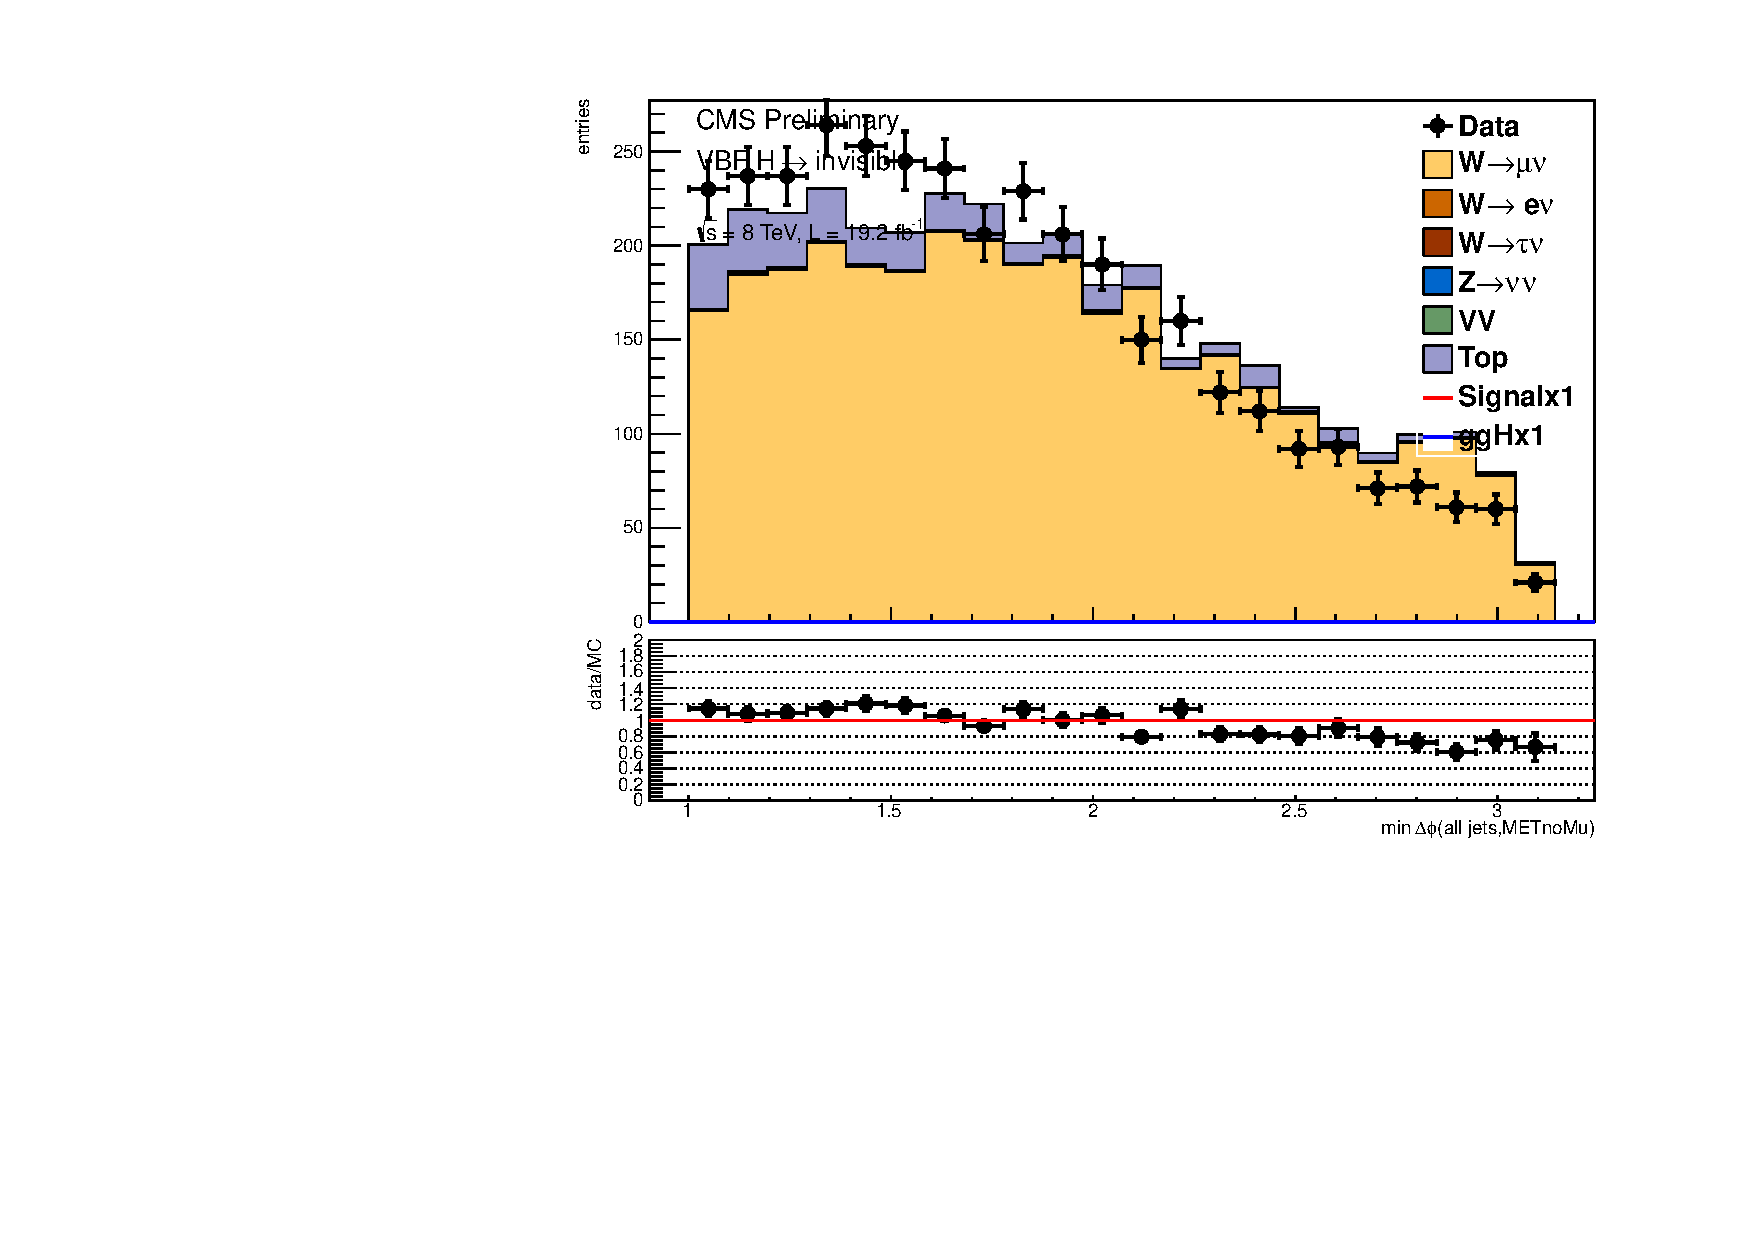
\includegraphics[clip=true,trim=0 0 0 20,width=.95\textwidth]{TalkPics/hig14038preapproval/output_presel/munu_alljetsmetnomu_mindphi.pdf}
  \end{columns}
\end{frame}

\begin{frame}
  \frametitle{Signal region selection}
   \begin{columns}
     \column{.55\textwidth}
     \begin{block}{}
       \scriptsize
       \begin{itemize}
       \item We optimise by choosing the cut values with the best 95\% C.L. expected limit
       \item[-] Limit calculation details later
       \item We scanned through jet 2 $p_{T}$, $\frac{METnoMU}{\sigma_{METnoMU}}$, $\text{Min}\Delta\phi(all\,jets\,,METnomu)$ and $M_{jj}$
       \item Best limit was found for:
       \item[-] jet 2 $p_{T}>45$ GeV
       \item[-] $\frac{METnoMU}{\sigma_{METnoMU}}>4$
       \item[-] $\text{Min}\Delta\phi(all\,jets,METnomu)>2.3$
       \item[-] $M_{jj}>1200$ GeV
       \item We defined this as our ``signal region''
       \item Discrepancy outside signal region is from QCD
       \end{itemize}
    \end{block}
    \column{.5\textwidth}
    \vspace{-.25cm}

    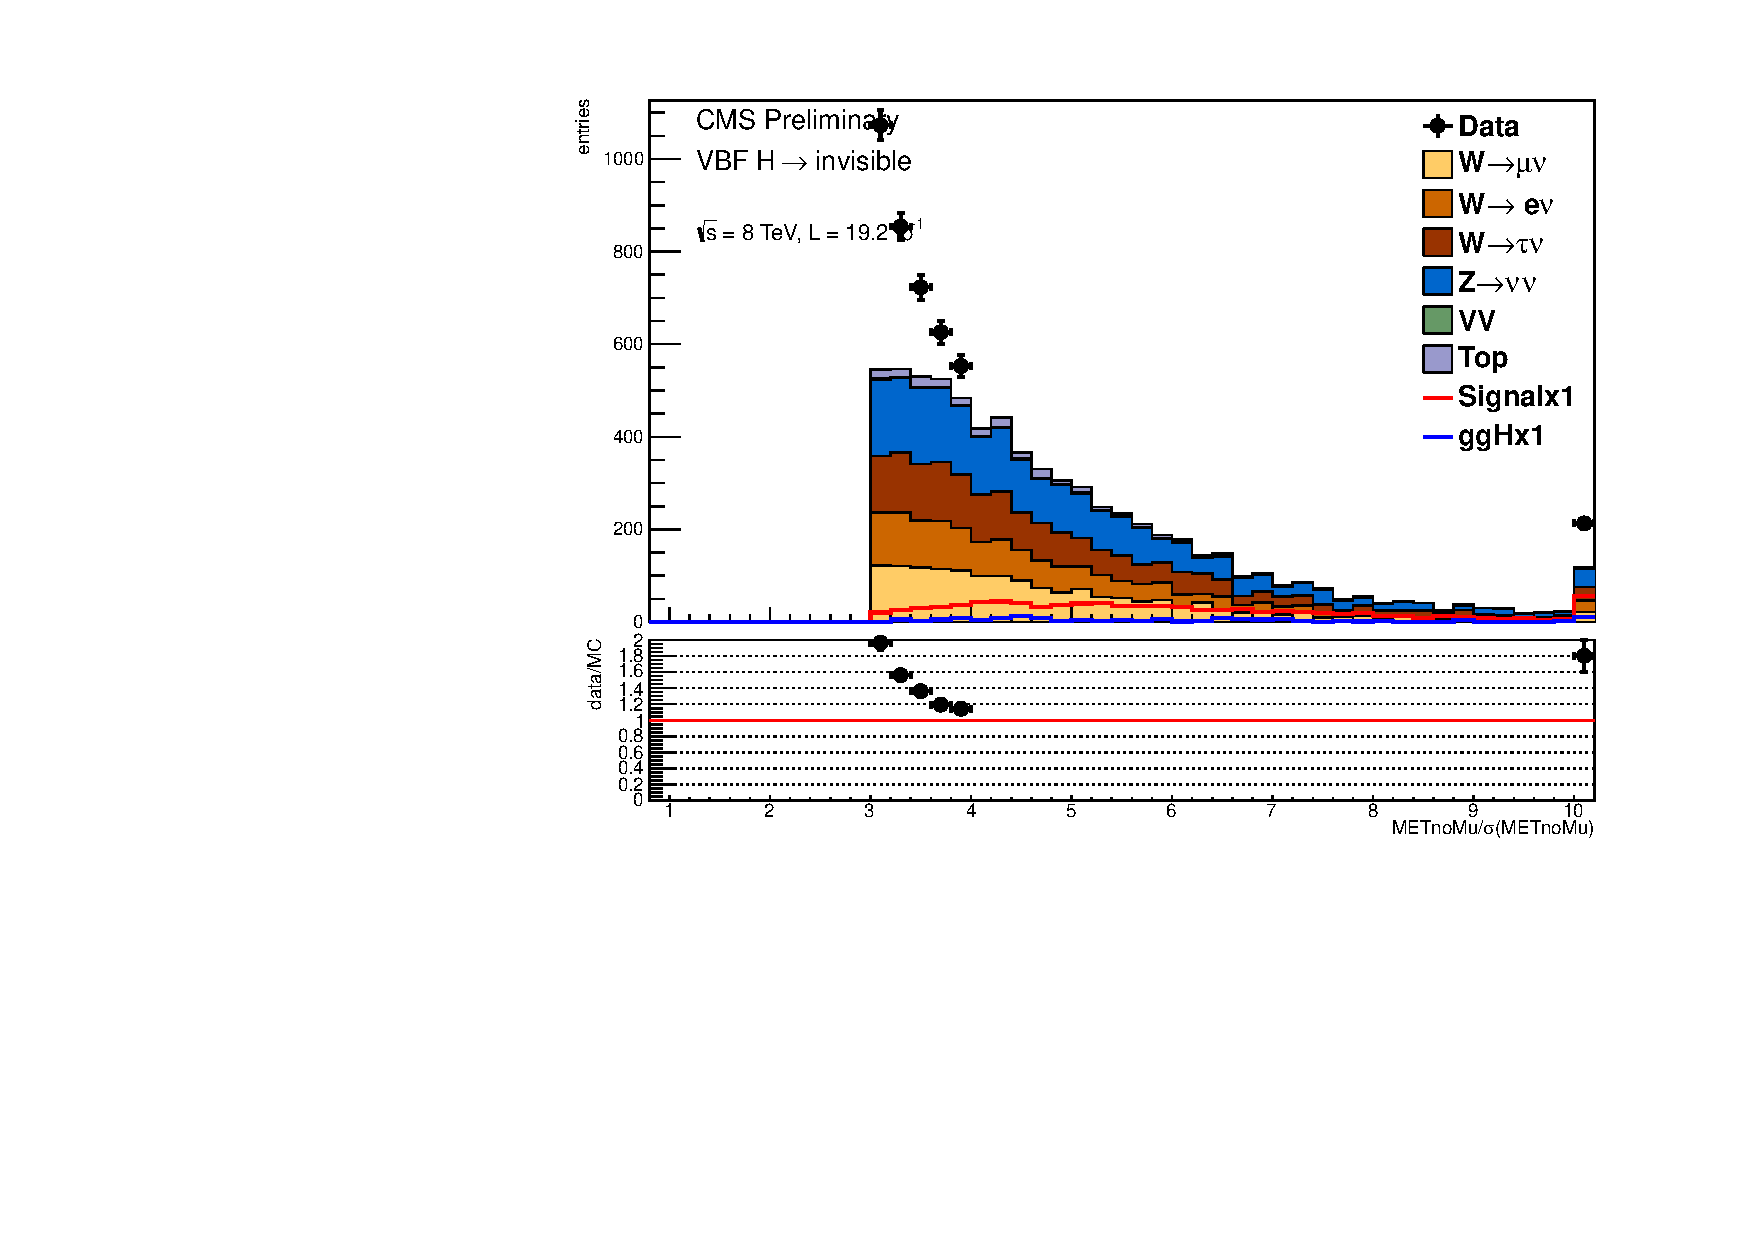
\includegraphics[clip=true,trim=0 0 0 20,width=.95\textwidth]{TalkPics/hig14038preapproval/output_presel/nunu_metnomu_significance.pdf}
    \vspace{-.05cm}
    

    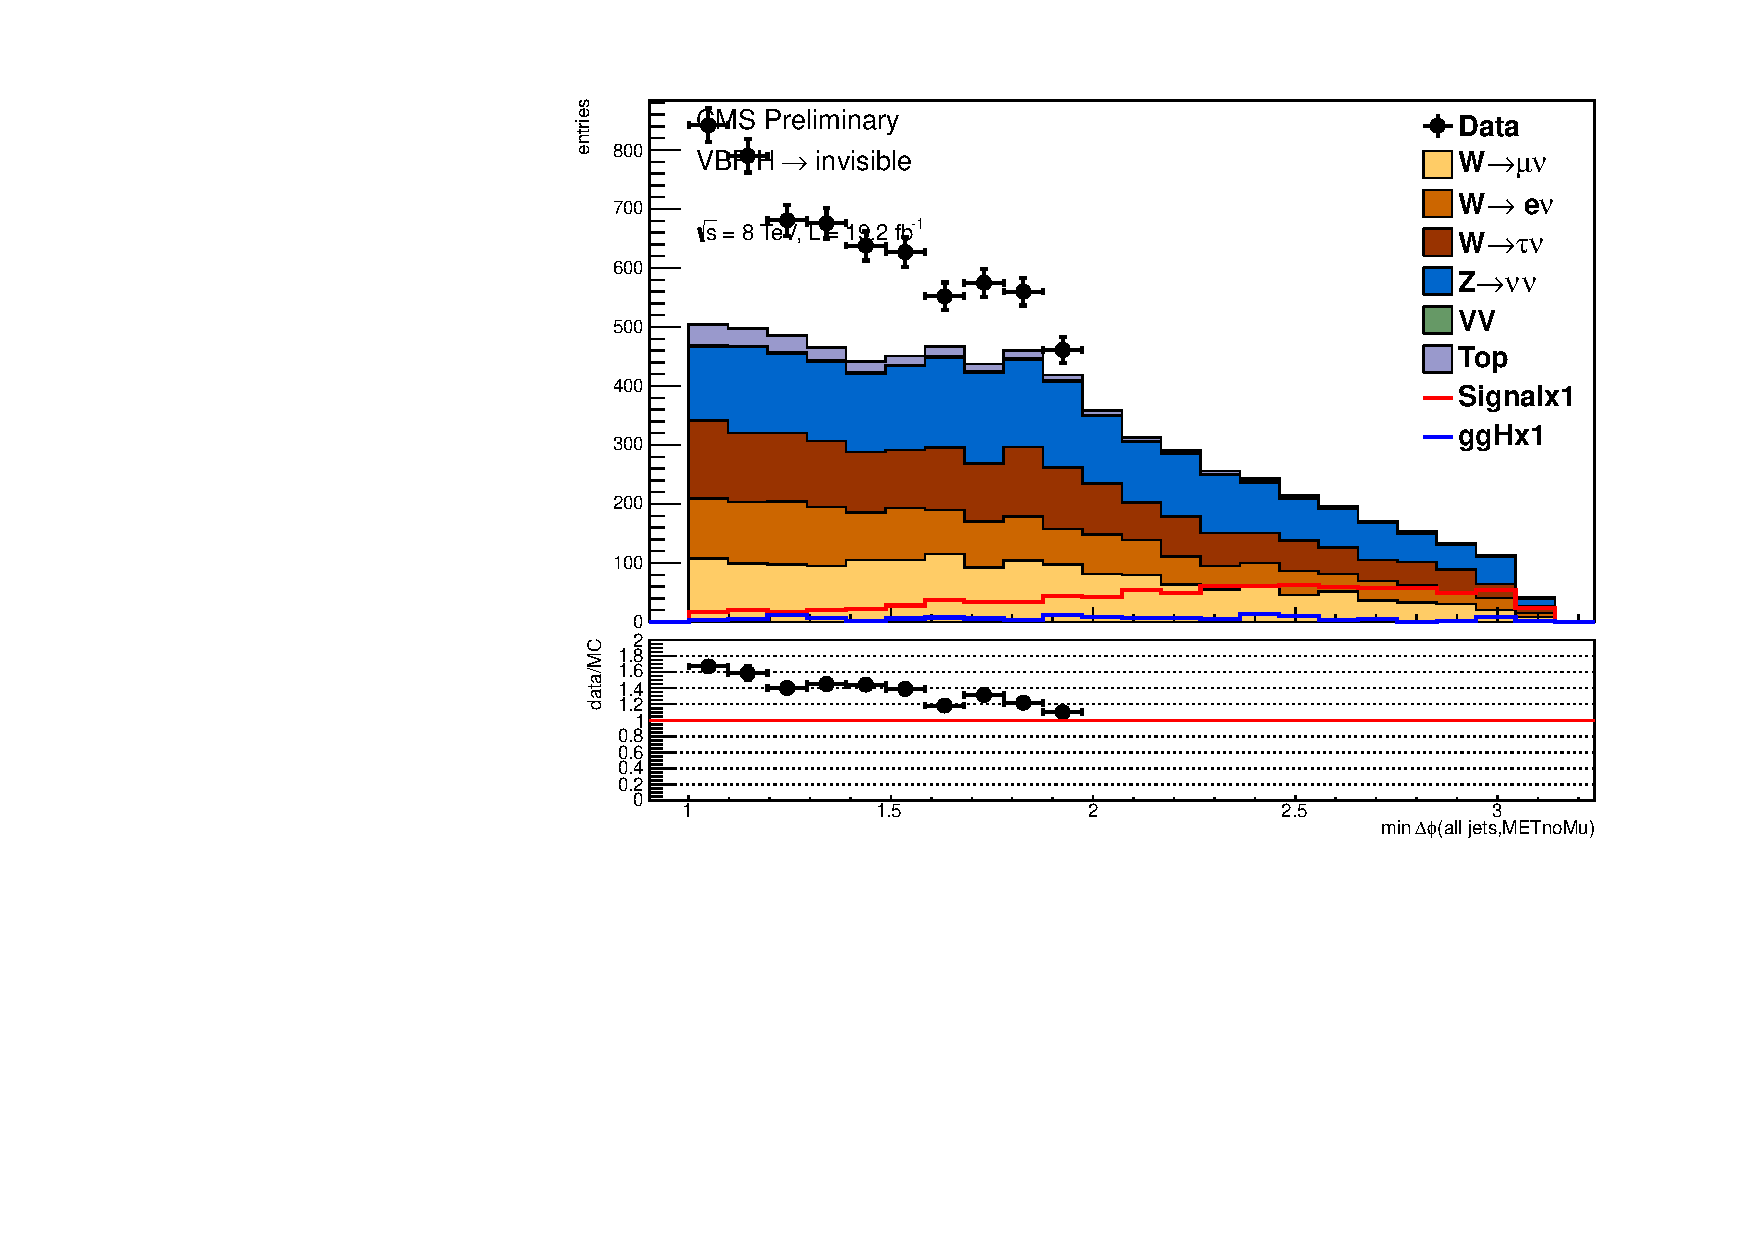
\includegraphics[clip=true,trim=0 0 0 20,width=.95\textwidth]{TalkPics/hig14038preapproval/output_presel/nunu_alljetsmetnomu_mindphi.pdf}
  \end{columns}
\end{frame}

%TOP CONTROL REGION
\begin{frame}
  \frametitle{Top control region}
  \vspace{-.3cm}

  \begin{columns}
    \column{1.08\textwidth}
  \begin{columns}
    \column{.52\textwidth}
    \begin{block}{}
      \scriptsize
      \begin{itemize}
      \item Top contribution to V+jets control regions is non-negligible
      \item Use method used for W backgrounds in prompt analysis
      \item Region: signal region with lepton veto replaced with requirement for 1 tight muon and 1 tight electron
      \item[-] Very few events in $e\mu$ region so also removed $\text{Min}\Delta\phi(all\,jets,\,METnomu)$ cut
      \end{itemize}
      \begin{tabular}{|l|c|}
        \hline
        $N_{C}^{data}$ & $21\pm 4.6 (\text{stat.})$\\
        $N_{C}^{bkg}$ & $0.3\pm 0.1 (\text{MC stat.})$  \\
        $N_{S}^{top\,MC}$ & $5.3\pm 1.3 (\text{MC stat.})$ \\
        $N_{C}^{top\,MC}$ & $24.6\pm 4.0  (\text{MC stat.})$   \\
        \hline
        \tiny $\frac{N^{data}-N^{bkg}}{N^{top\,MC}_{C}}$ & \scriptsize $0.8 \pm 0.2(stat.)\pm0.1(MC stat.)$ \\
        \hline
        $N_{S}^{top}$ & \textcolor{red}{$4.4\pm 1.0 (\text{stat.}) \pm 1.3 (\text{MC stat.})$} \\ 
        \hline
\end{tabular}
    \end{block}
    \column{.49\textwidth}
    \vspace{.1cm}
    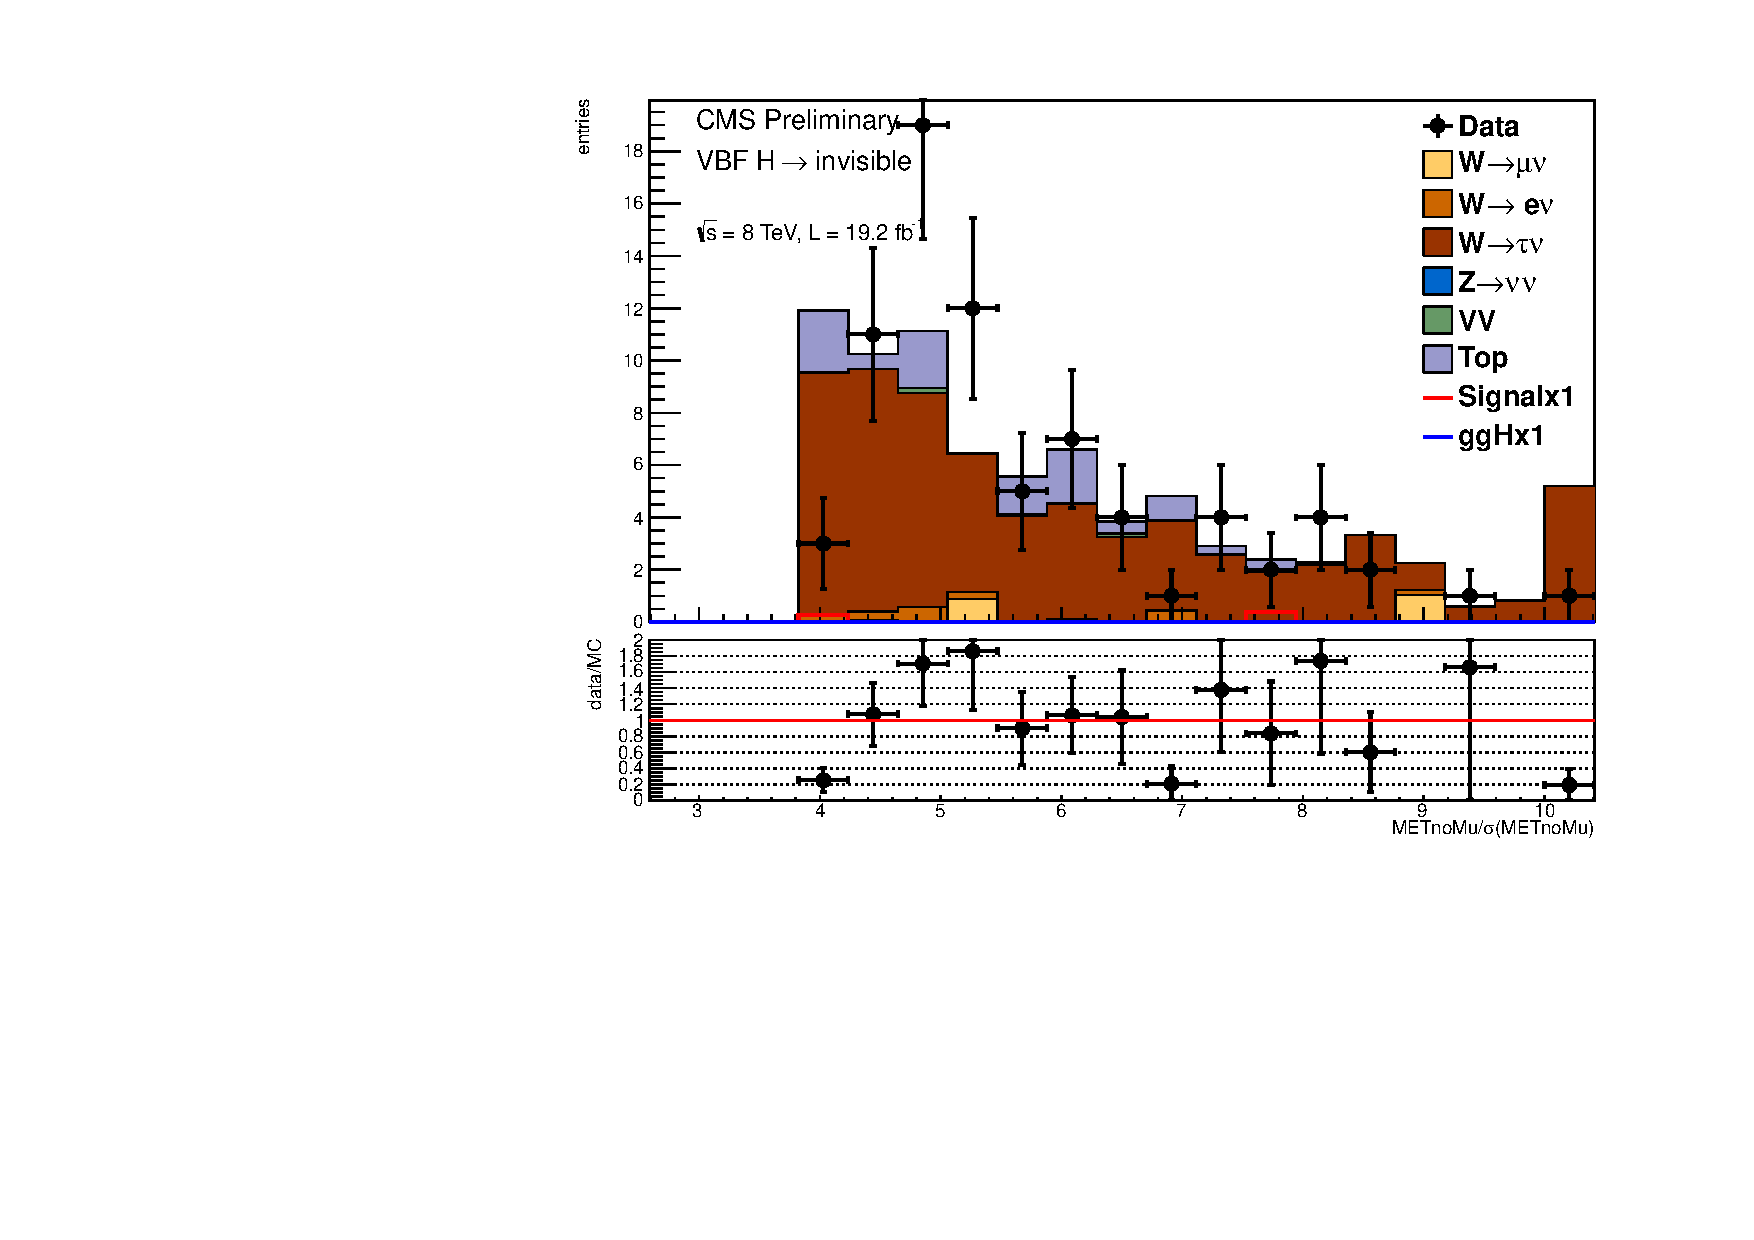
\includegraphics[clip=true,trim=0 100 0 0,width=\textwidth]{TalkPics/hig14038preapproval/output_sigreg/taunu_metnomu_significance.pdf}
    \vspace{-.3cm}

    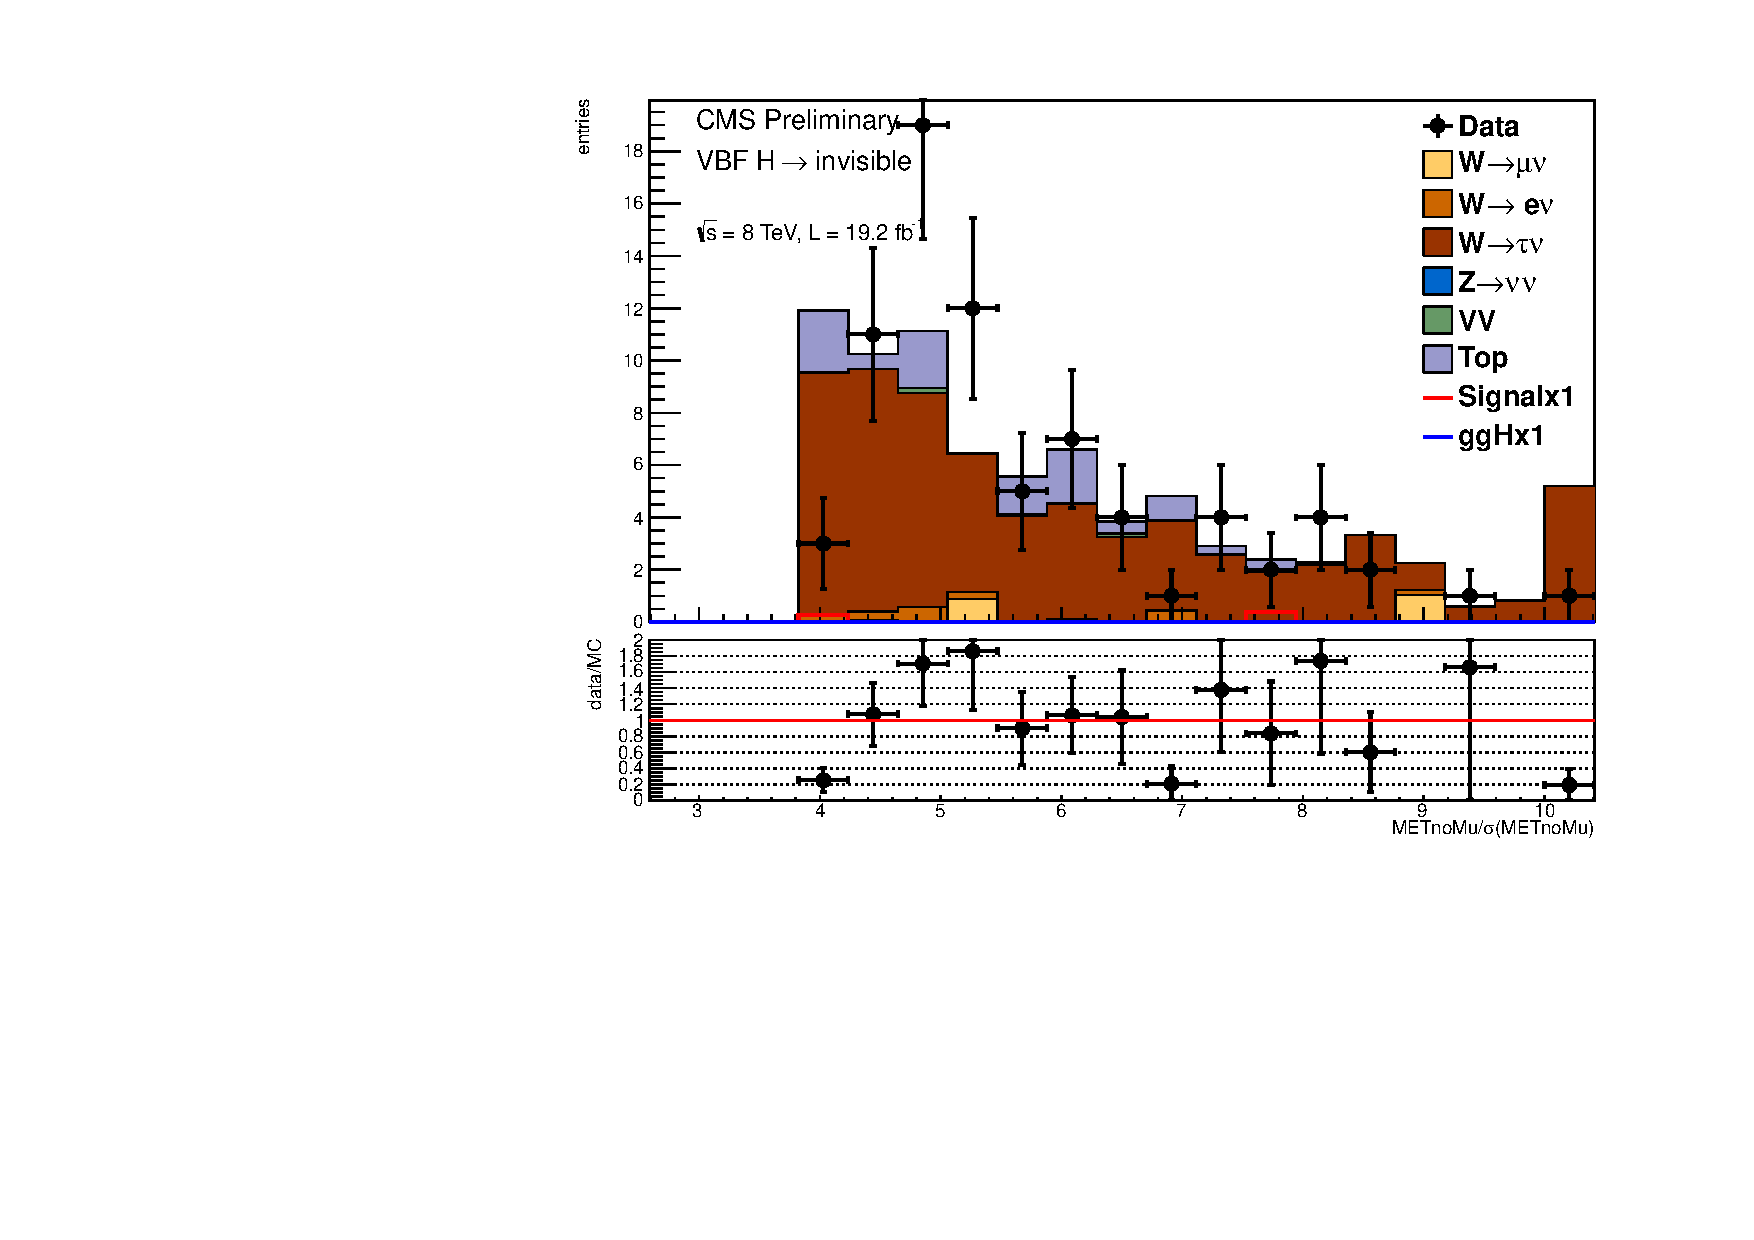
\includegraphics[clip=true,trim=0 0 0 360,width=\textwidth]{TalkPics/hig14038preapproval/output_sigreg/taunu_metnomu_significance.pdf}
    
    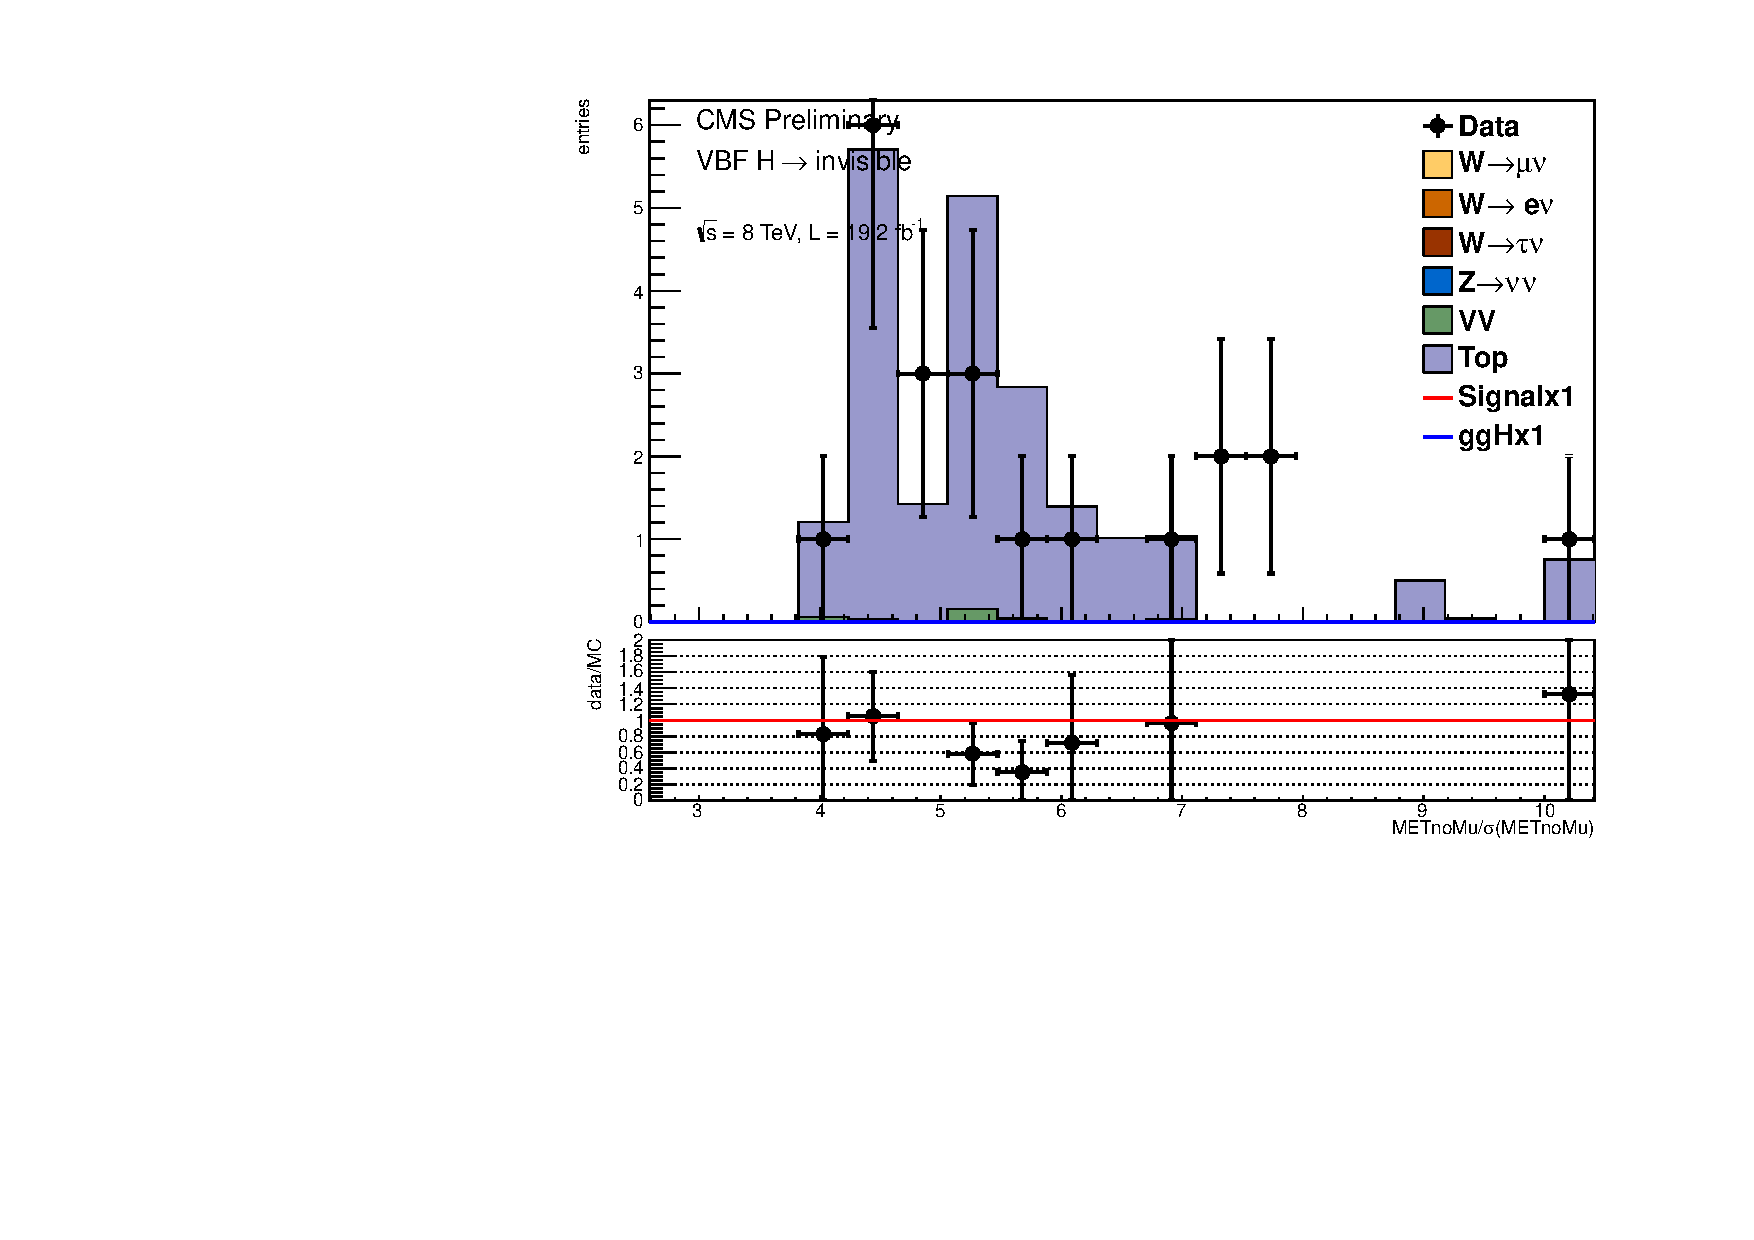
\includegraphics[clip=true,trim=0 0 0 20,width=\textwidth, height=.45\textheight]{TalkPics/hig14038preapproval/output_sigreg/top_metnomu_significance.pdf}
  \end{columns}
  \end{columns}
\end{frame}

\begin{frame}
  \frametitle{$W\rightarrow e\nu$, $W\rightarrow\mu\nu$, $Z\rightarrow\nu\nu$}
  \vspace{-.2cm}
  \begin{block}{}
    \scriptsize
    \begin{itemize}
      \vspace{-.1cm}
    \item Data-MC agreement good
    \item Same method used as for prompt analysis
    \item Details in backup
    \end{itemize}
    \vspace{-.2cm}
    \centering
    \begin{tabular}{|l|c|}
      \hline
      Background& Number of events \\
      \hline
      $W\rightarrow e\nu$&\textcolor{red}{$57.4\pm7.3$(stat.)$\pm5.9$(MC stat.)} \\
      $W\rightarrow\mu\nu$&\textcolor{red}{$101.8\pm6.1$(stat.)$\pm8.3$(MC stat.)}\\
      $Z\rightarrow\nu\nu$ & \textcolor{red}{$157.3 \pm 37.6 (data stat.) \pm 18.2 (MC stat.)$} \\      
      \hline
    \end{tabular}

  \end{block}

  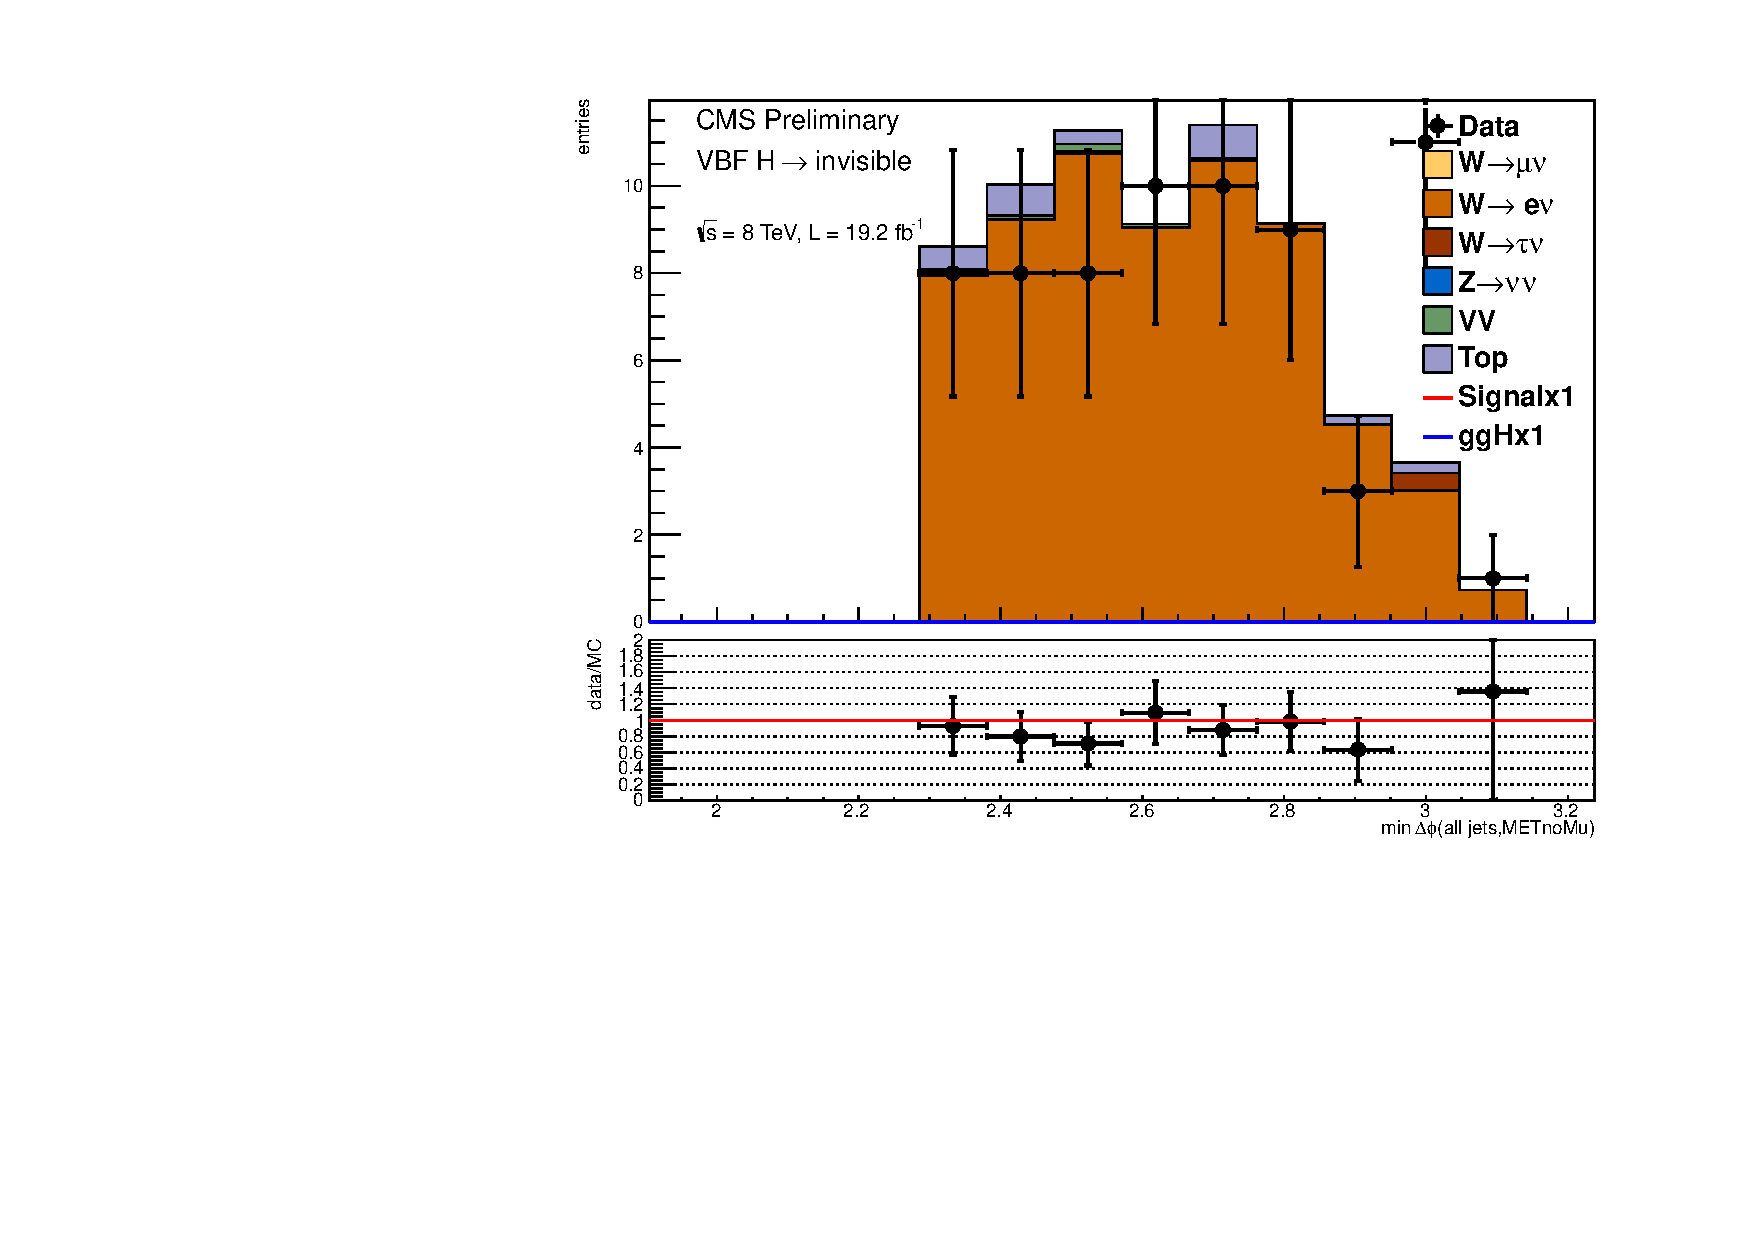
\includegraphics[clip=true,trim= 0 0 0 20,width=.33\textwidth]{TalkPics/hig14038preapproval/output_sigreg/enu_alljetsmetnomu_mindphi}
  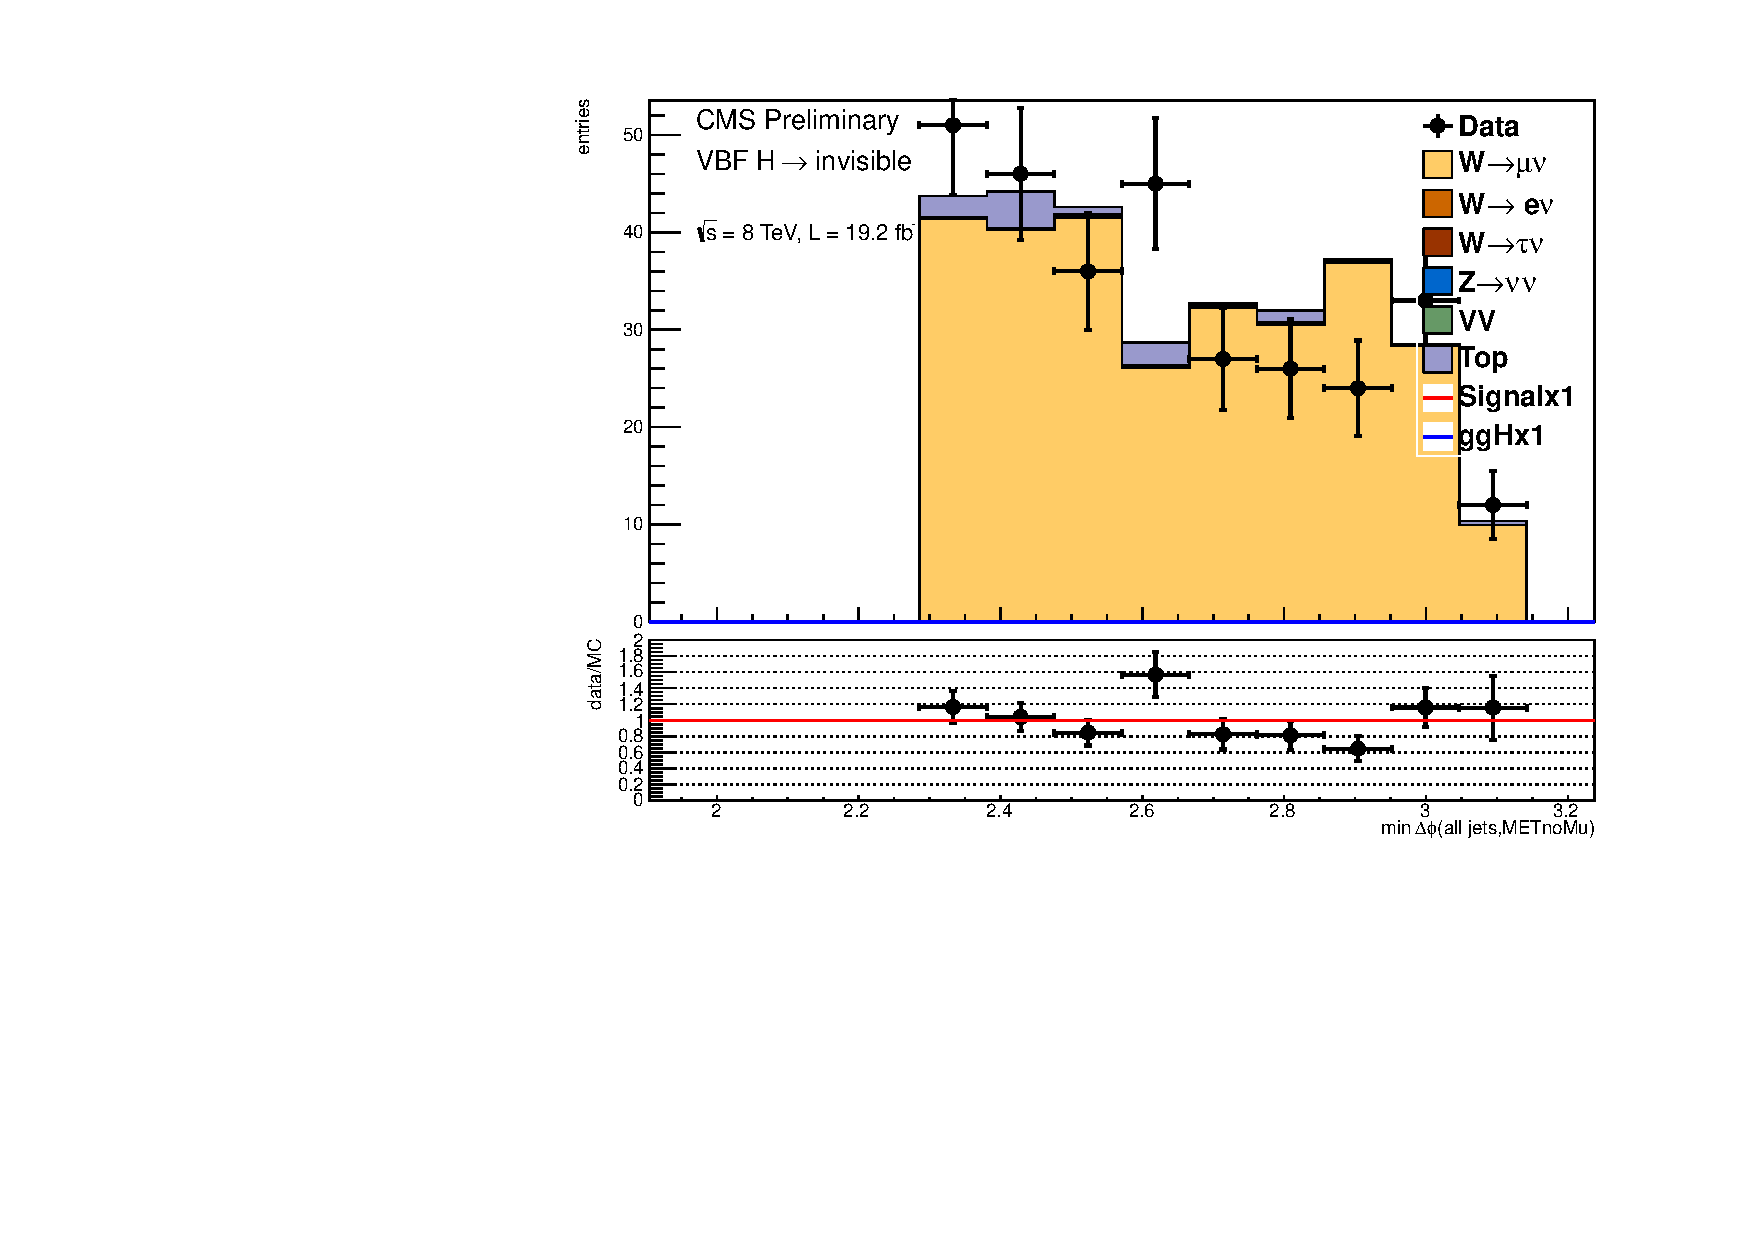
\includegraphics[clip=true,trim= 0 0 0 20,width=.33\textwidth]{TalkPics/hig14038preapproval/output_sigreg/munu_alljetsmetnomu_mindphi}
  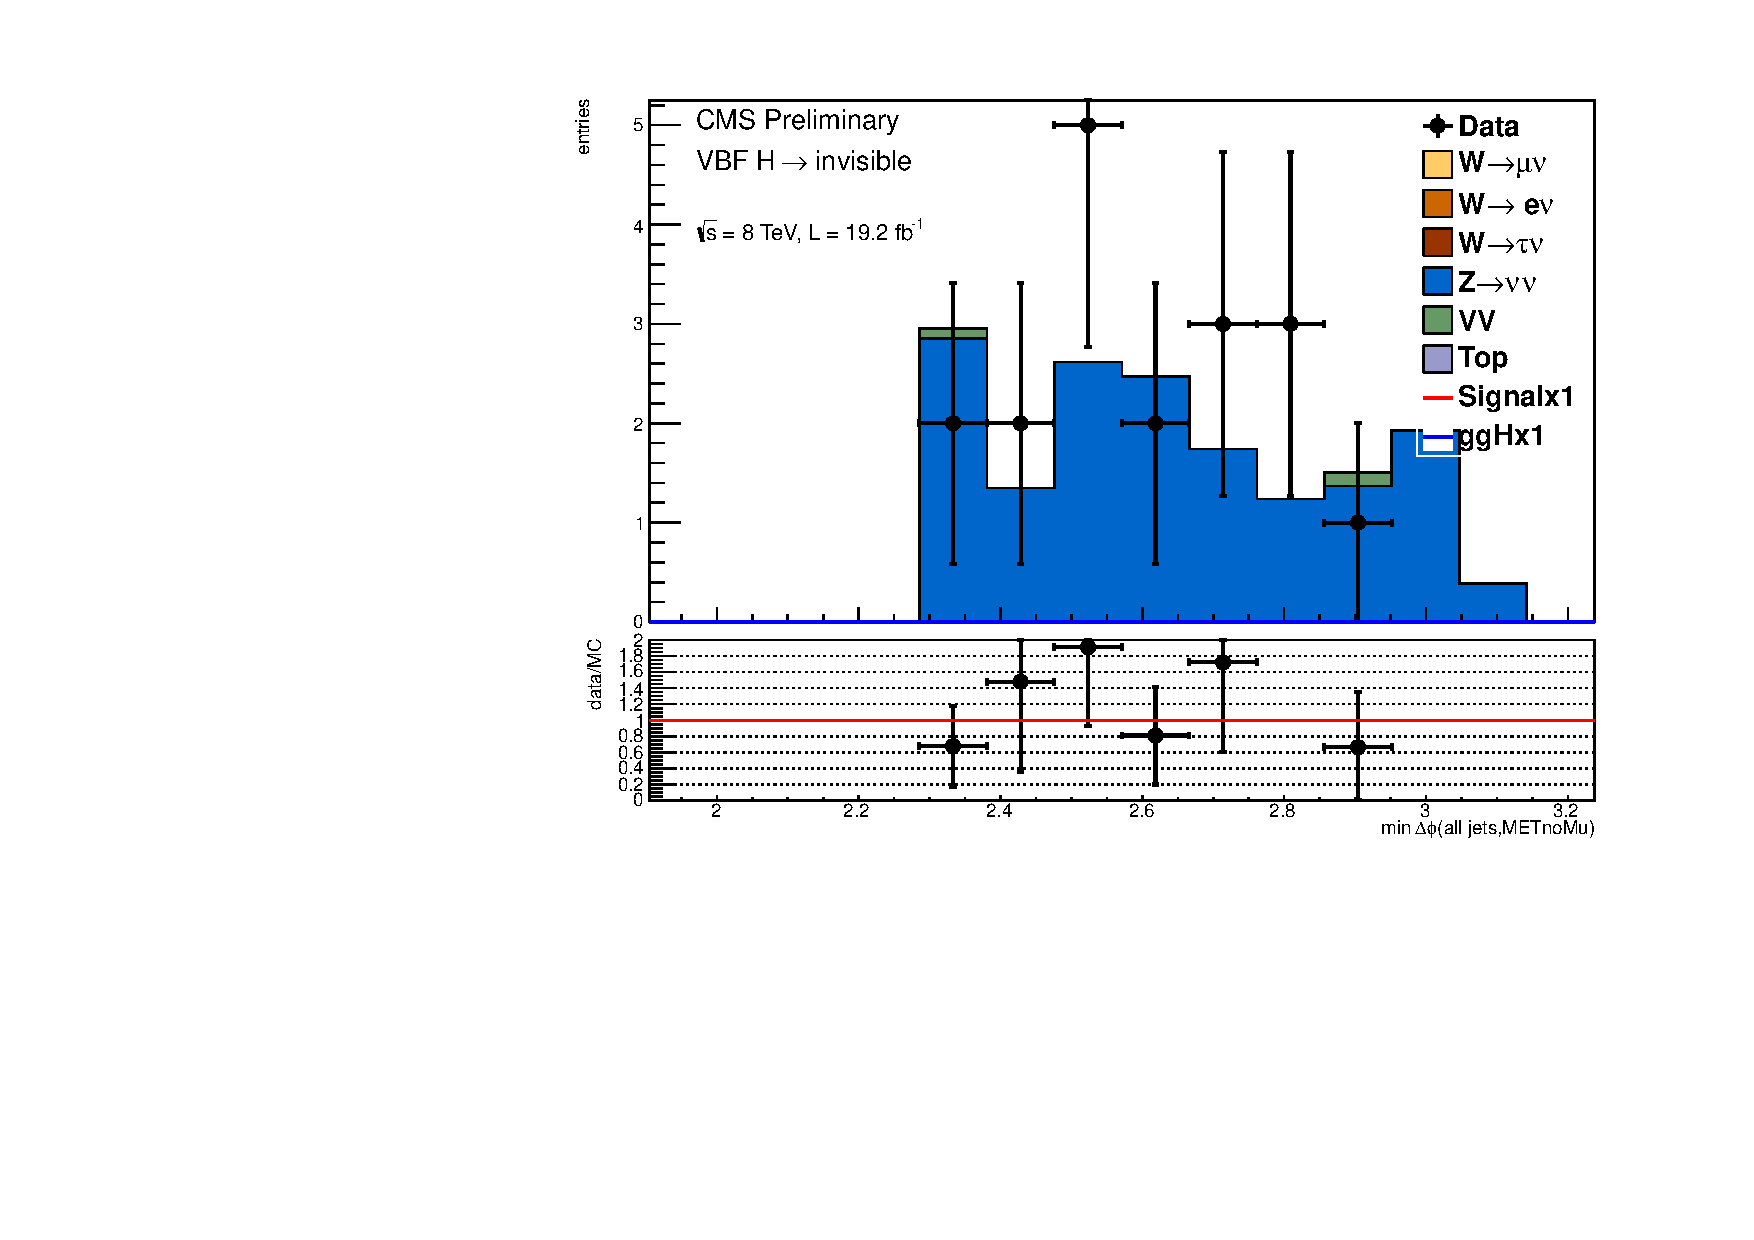
\includegraphics[clip=true,trim= 0 0 0 20,width=.33\textwidth]{TalkPics/hig14038preapproval/output_sigreg/mumu_alljetsmetnomu_mindphi}

  
\end{frame}

\begin{frame}
  \frametitle{$W\rightarrow\tau\nu$ control region}
  \begin{columns}
    \column{.55\textwidth}
    \vspace{-.2cm}
    \begin{block}{}
      \scriptsize
      \begin{itemize}
      \item Control regions for other W backgrounds:
      \item[-] signal region with lepton veto replaced with a requirement for a single lepton
      \item For $W\rightarrow\tau\nu$ there are not enough events in this region:
        \vspace{-.1cm}
      \item Remove the $\text{Min}\Delta\phi(all\,jets,\,METnomu)$ cut
      \item This leads to QCD contamination so we require:
        \vspace{-.1cm}
      \item[-] $\text{Min}\Delta\phi(leading\,2\,jets,\,METnomu)>1.0$
        \vspace{-.1cm}
      \item[-] $m_{T}$ of the lepton-MET system $>20$ GeV
      \item We add a 20\% systematic on the $W\rightarrow\tau\nu$ background
      \item Final $W\rightarrow\tau\nu$ estimate: $98.0 \pm 13.2 (stat.) \pm 12.6 (MC stat.)$ 
      \end{itemize}
    \end{block}
    \column{.5\textwidth}
    \vspace{-.1cm}

    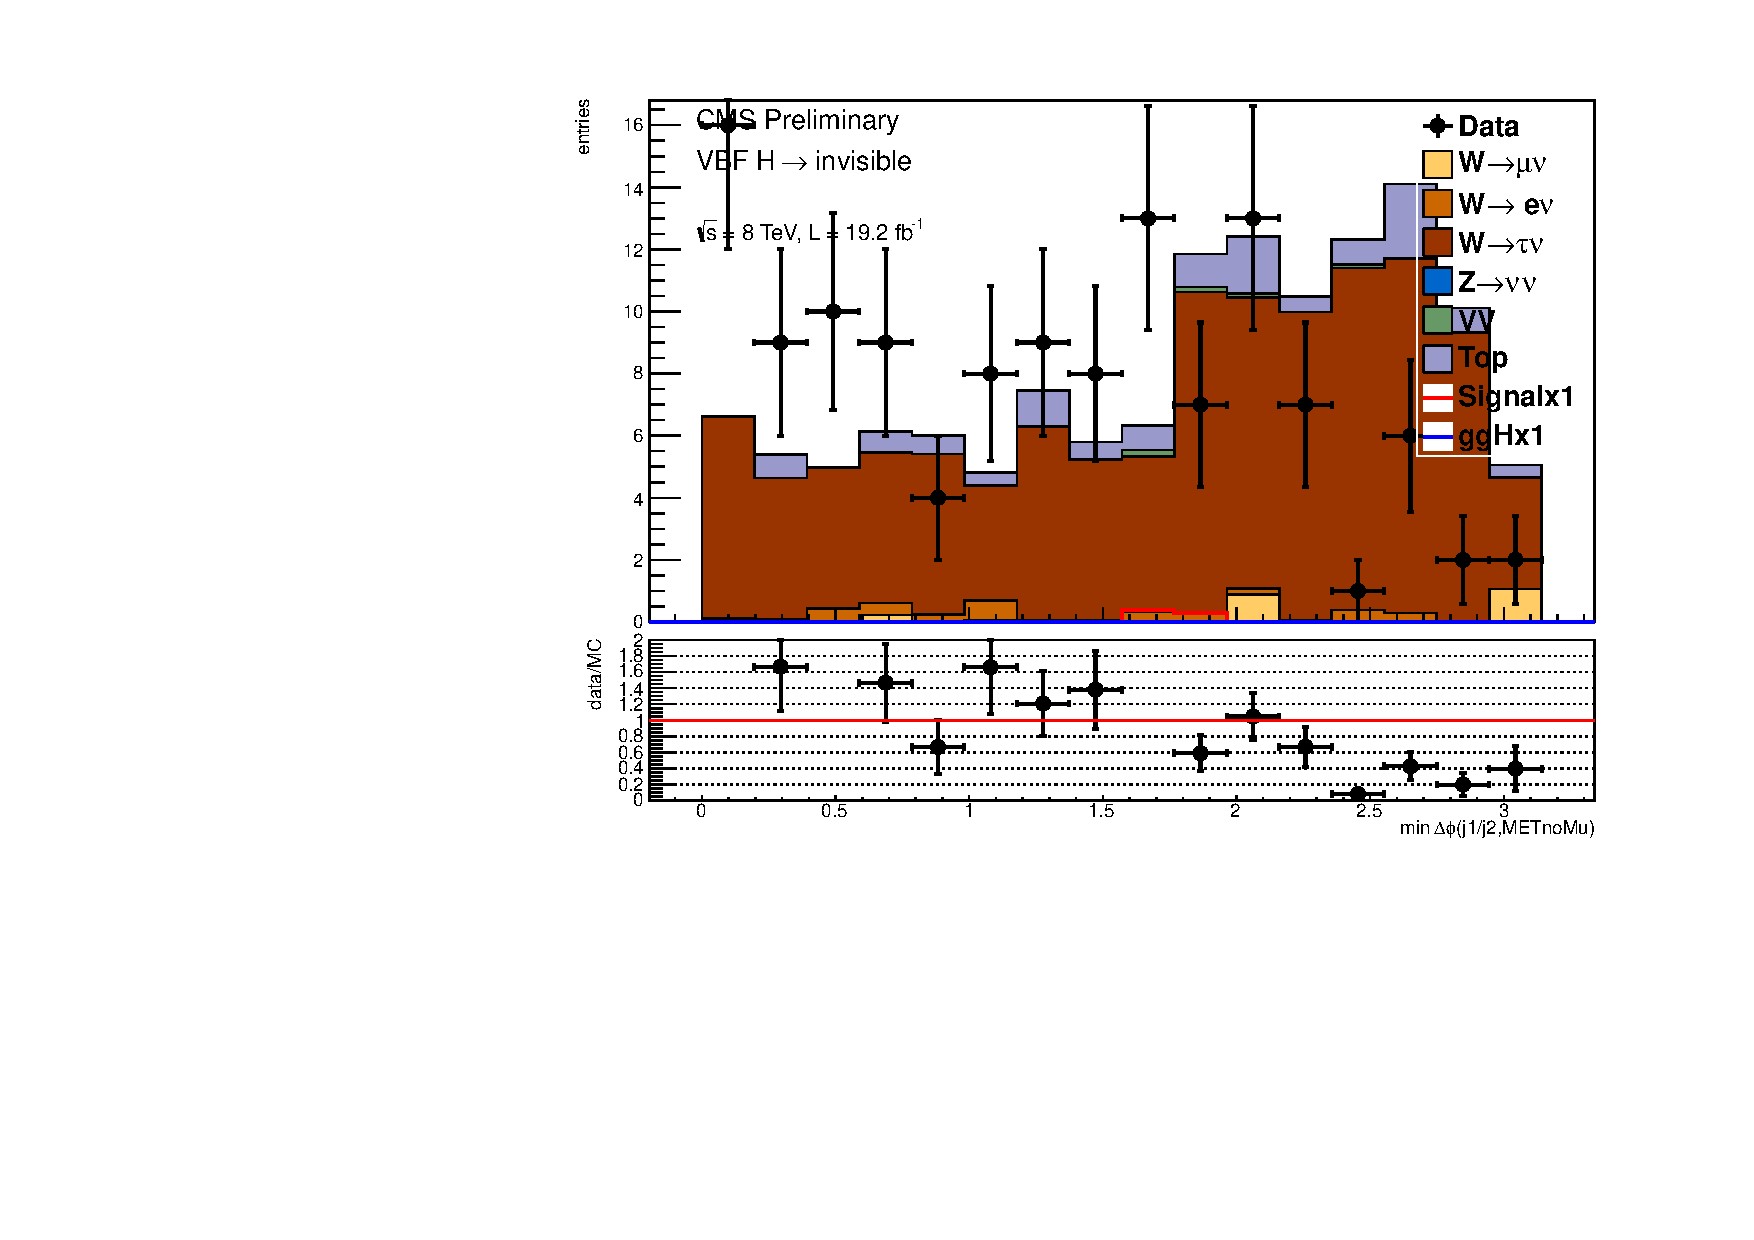
\includegraphics[clip=true,trim=0 0 0 20,width=.95\textwidth]{TalkPics/hig14038preapproval/taununoleadingjetmetdphicut.pdf}
    
    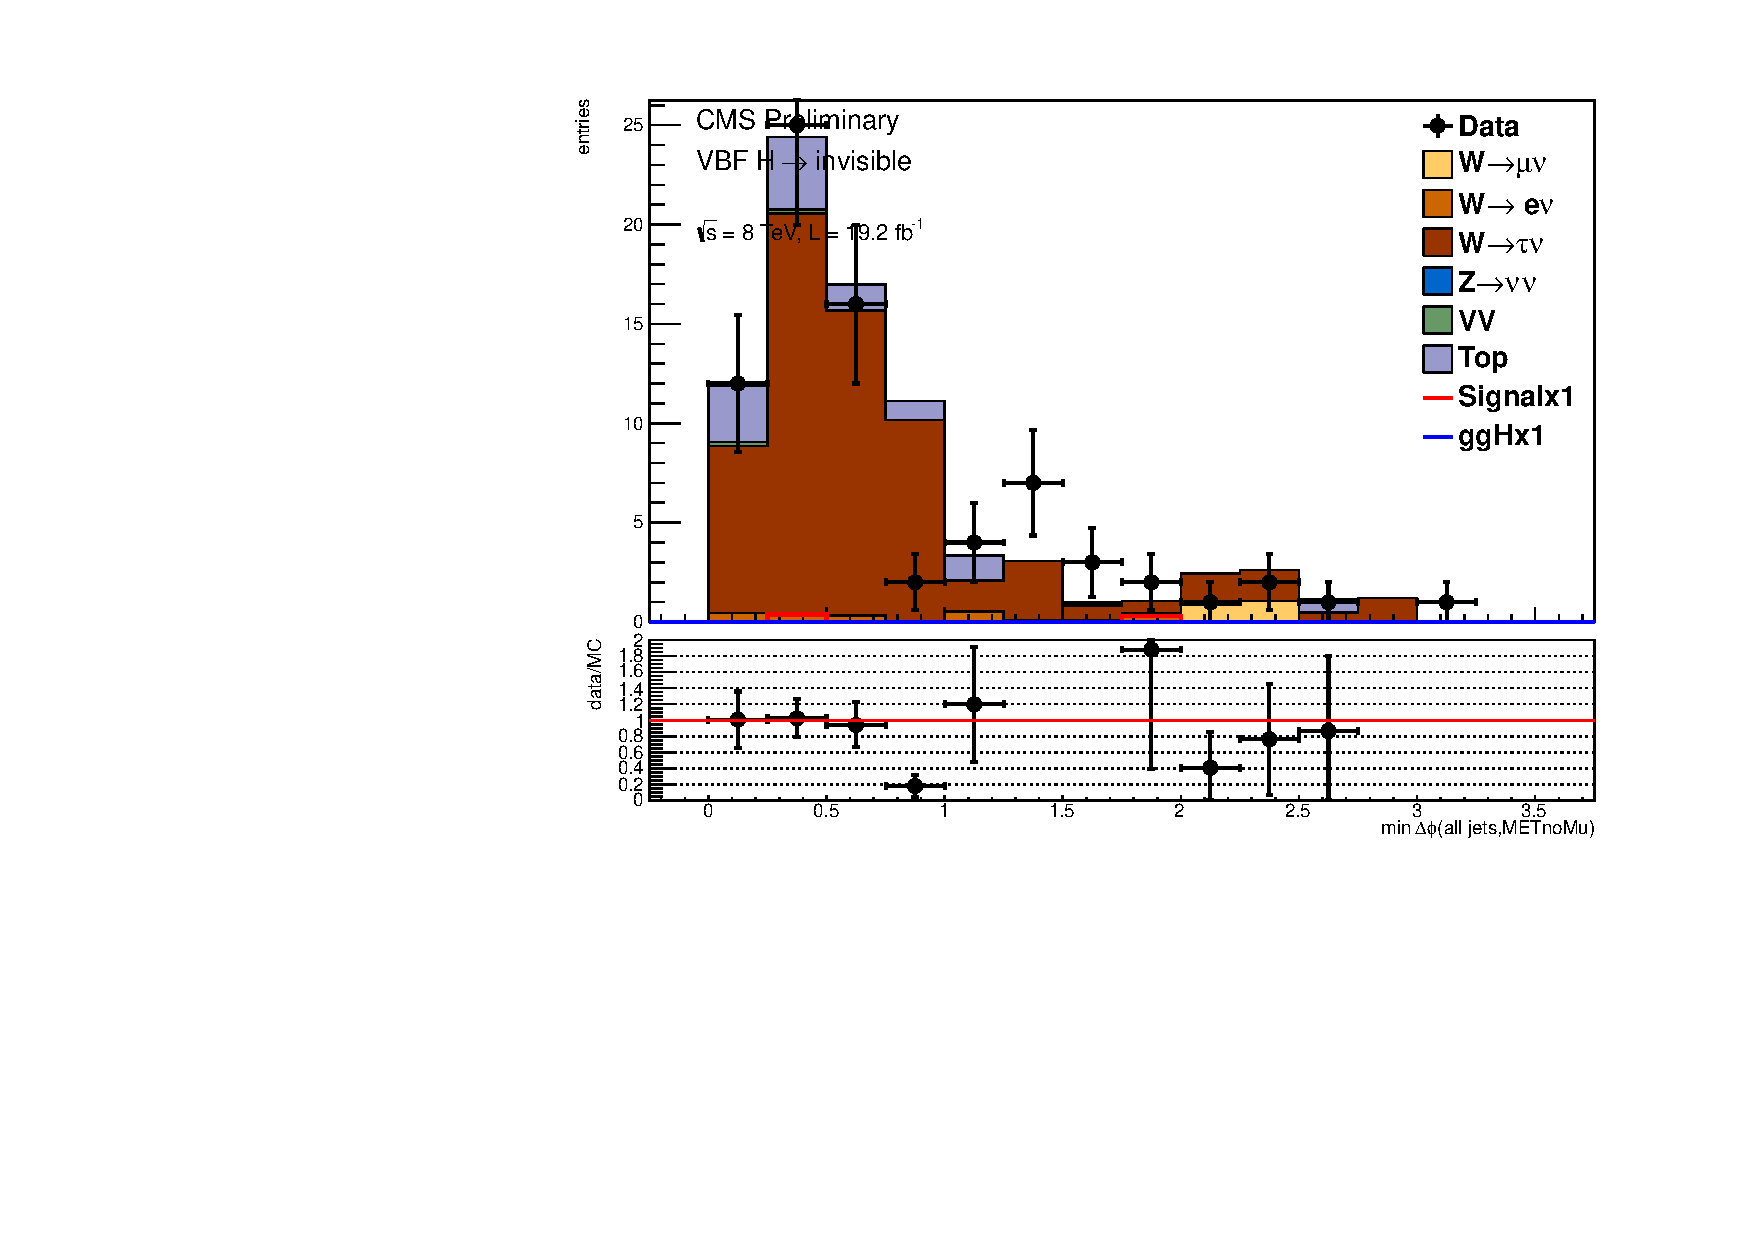
\includegraphics[clip=true,trim=0 0 0 20,width=.95\textwidth]{TalkPics/hig14038preapproval/output_sigreg/taunu_alljetsmetnomu_mindphi.pdf}
  \end{columns}
\end{frame}


\begin{frame}
  \frametitle{QCD background estimation: Shape}
   \begin{columns}
     \column{.55\textwidth}
     \begin{block}{}
       \scriptsize
       \begin{itemize}
       \item Other background methods estimate unreconstructed contribution from reconstructed
       \item For QCD use MET near reconstructed jets to model MET from unreconstructed/mismeasured jets
       \item Use region with low $\text{Min}\Delta\phi(all\,jets,\,METnomu)$ but high $\text{Min}\Delta\phi(leading\,jets,\,METnomu)$
       \item[-] $\text{Min}\Delta\phi(all\,jets,\,METnomu)<1.0$
       \item[-] $\text{Min}\Delta\phi(leading\,jets,\,METnomu)>1.0$ 
       \item Has good shape agreement with enriched QCD MC
       \item Use shape from this region
       \end{itemize}
     \end{block}
     \column{.5\textwidth}
     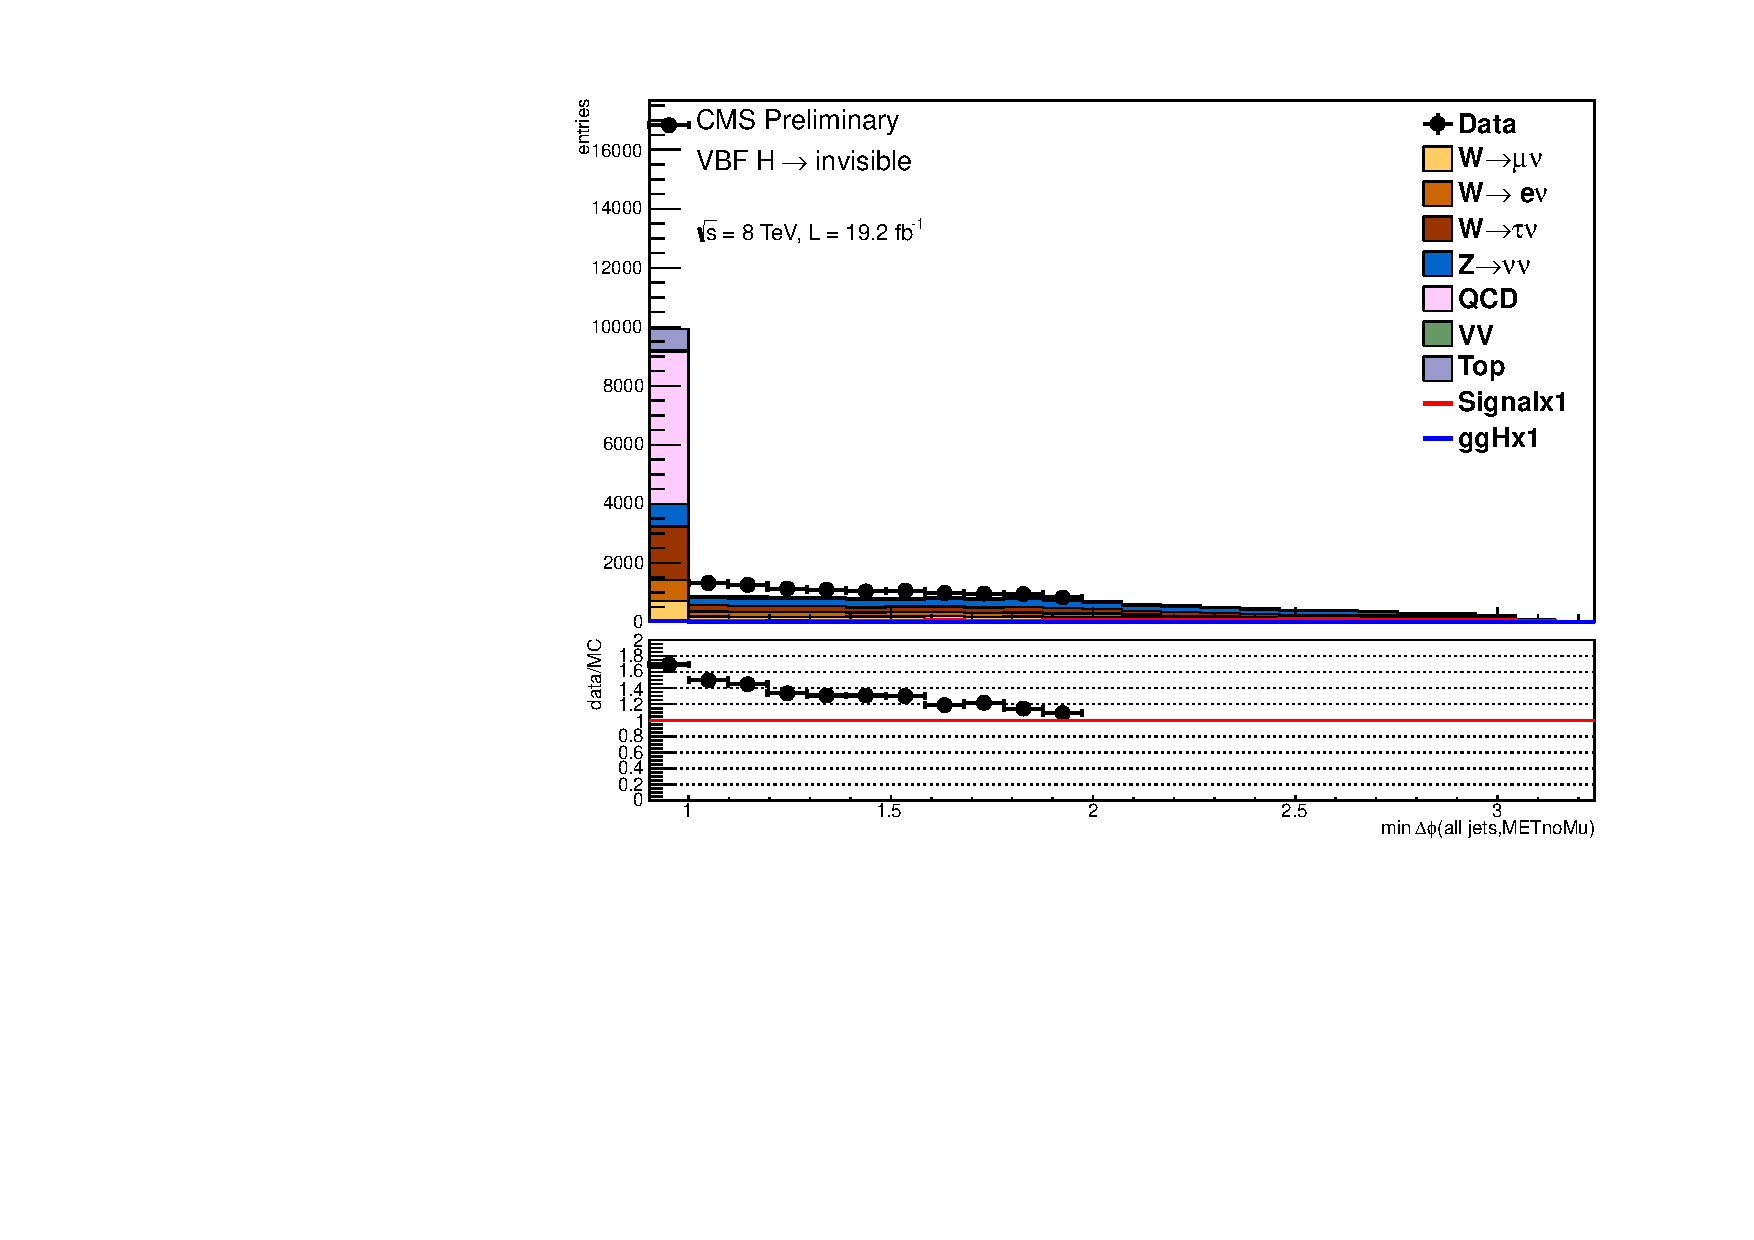
\includegraphics[clip=true,trim=0 0 0 20,width=.95\textwidth]{TalkPics/hig14038preapproval/output_amqcd/nunu_alljetsmetnomu_mindphi.pdf}
     
     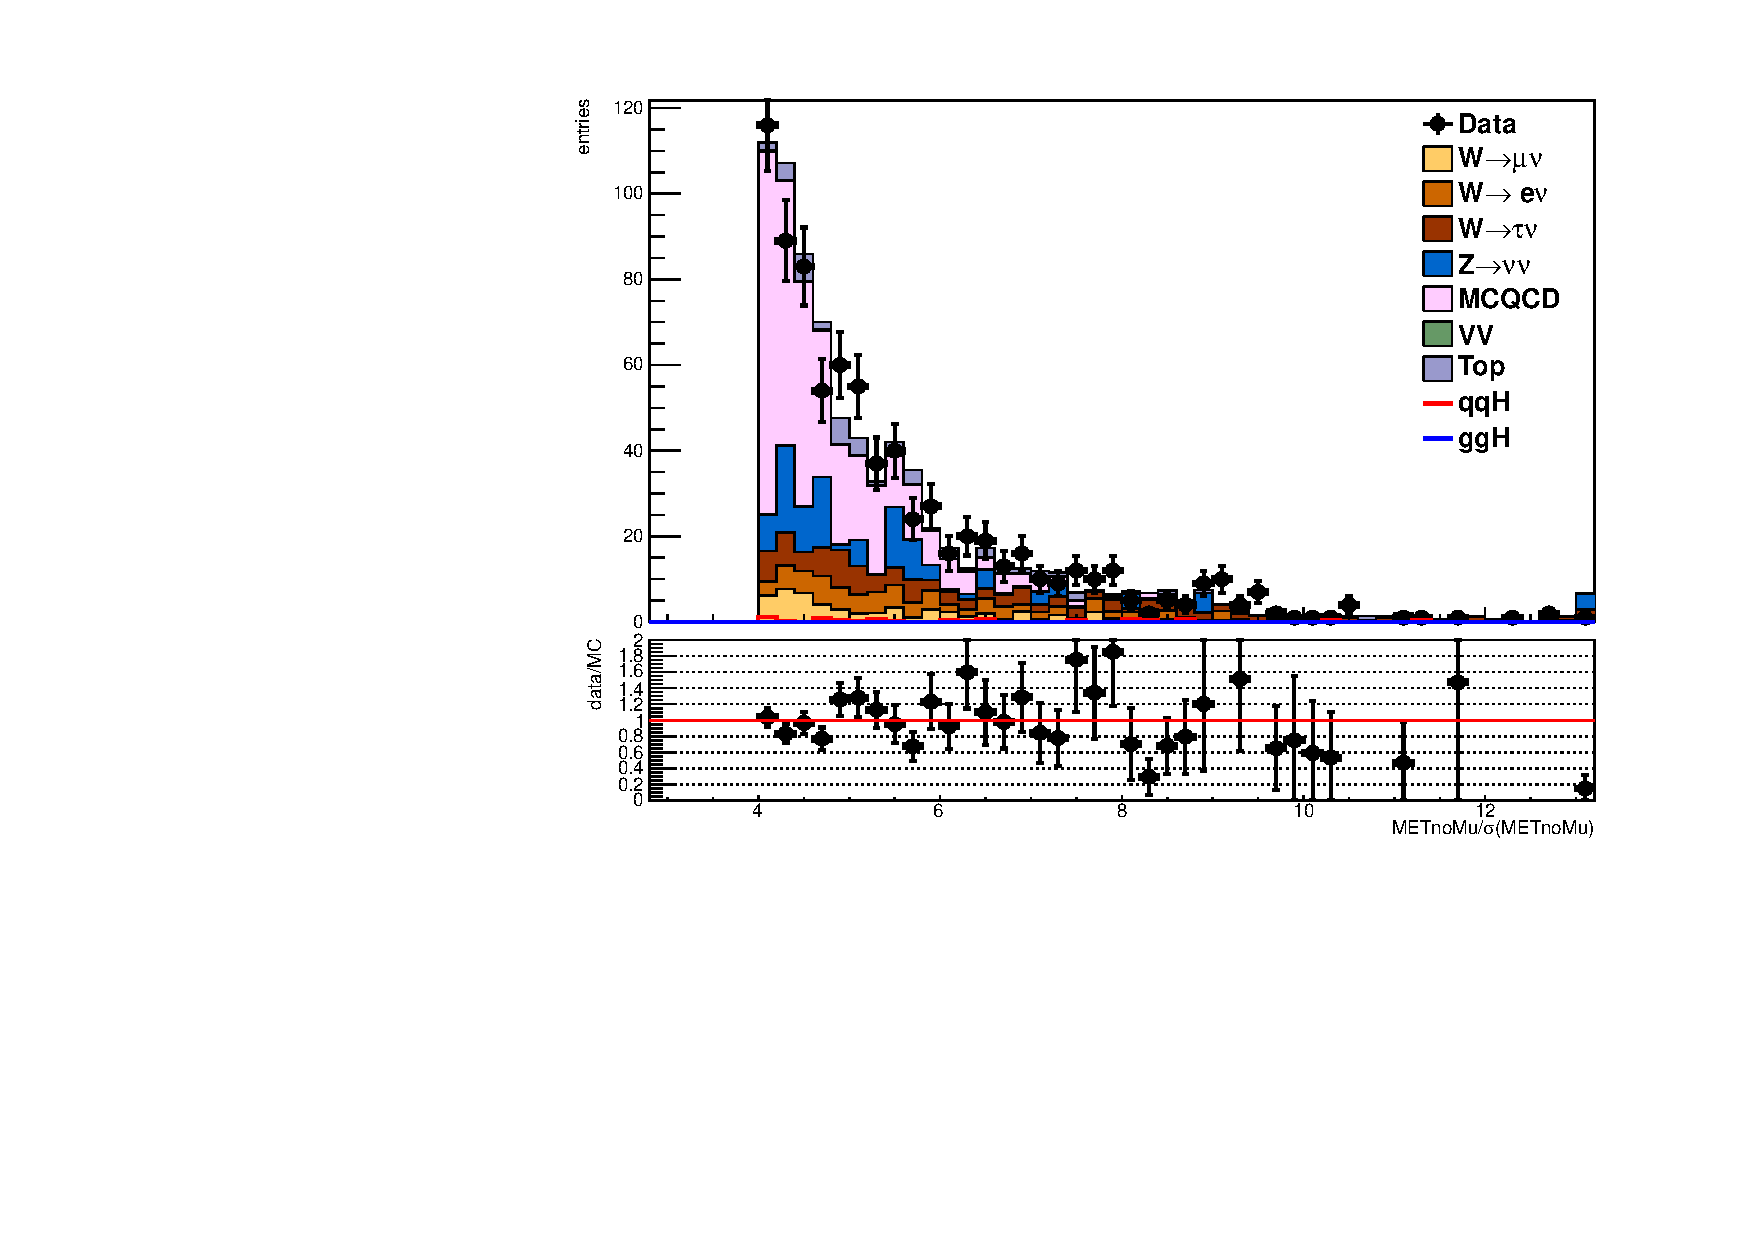
\includegraphics[clip=true,trim=0 0 0 20,width=.95\textwidth]{TalkPics/hig14038preapproval/output_invqcd/qcd_metnomu_significance.pdf}
     
   \end{columns}
\end{frame}

\begin{frame}
  \frametitle{QCD background estimation: Normalisation}
  \vspace{-.2cm}
     \centering
      \tiny
      \begin{tabular}{c r}
        &   \\
        \multirow{4}{*}{$\text{min}\Delta\phi(METnomu,\text{j1/j2})$} & \\
        & \multirow{2}{*}{2.3} \\
        &  \\
        & \multirow{2}{*}{2.0}  \\
        & \\
        & \multirow{2}{*}{1.0}\\
        \multirow{2}{*}{$\text{min}\Delta\phi(METnomu,\text{all jets})$} & \\
        & \multirow{2}{*}{0.0}\\
        & \\
        & \\
      \end{tabular}
       \begin{tabular}{c c c | c c c c}
         \multicolumn{7}{|c}{}\\
         \multicolumn{3}{|c|}{{\cellcolor{cyan}}} & \multicolumn{3}{|c}{\cellcolor{green}} & \\
         \multicolumn{3}{|c|}{{\cellcolor{cyan}}} & \multicolumn{3}{|c}{\multirow{-2}{*}{\cellcolor{green}Signal}}  & \multirow{4}{*}{} \\
         \cline{4-7}
         \multicolumn{3}{|c|}{\multirow{-2}{*}{{\cellcolor{cyan}} Norm 2}} & \multicolumn{3}{|c}{} & \\
         \multicolumn{3}{|c|}{\multirow{-2}{*}{{\cellcolor{cyan}}}} & \multicolumn{3}{|c}{} & \\
         \hline
         \multicolumn{3}{|c|}{{\cellcolor{cyan}}} & \multicolumn{3}{|c}{\cellcolor{cyan}} & \\
         \multicolumn{3}{|c|}{\multirow{-2}{*}{{\cellcolor{cyan}}Norm 1}} & \multicolumn{3}{|c}{\multirow{-2}{*}{\cellcolor{cyan}Norm 3}} & \\
         \hline
         \hline
         \multicolumn{3}{|c|}{} & \multicolumn{3}{|c}{\cellcolor{orange}} & \\
         \multicolumn{3}{|c|}{} & \multicolumn{3}{|c}{\multirow{-2}{*}{\cellcolor{orange}QCD shape}} & \multirow{-2}{*}{} \\
         \hline
         \multicolumn{2}{l}{\hspace{-.4cm}3.0}  & \multicolumn{2}{c}{\hspace{.55cm}4.0} &  & \multicolumn{2}{c}{} \\
         \multicolumn{6}{c}{MET significance} & \\
       \end{tabular}

      \begin{block}{}
        \scriptsize
        \begin{itemize}
        \item MET significance and $\text{min}\Delta\phi(METnomu,\text{all jets})$ correlated
        \item[-] Cannot use ABCD to normalise
        \item Normalisation shows strong dependence on cut variables
        \item Fit normalisation variation in norm 1
        \item Check consistency in norm 2 and 3
        \item Final prediction: $N_{S}^{QCD}=17\pm 14$ 
        \end{itemize}
      \end{block}



\end{frame}

\begin{frame}
  \frametitle{Results}
    \begin{columns}
      \column{.7\textwidth}
  \begin{block}{}
    \scriptsize
    \centering
\begin{tabular}{|l|c|}
            \hline
            Background       & $N_{est} \pm (stat) \pm (syst)$ \\
            \hline
            $Z\rightarrow\nu\nu$&$157.3 \pm 37.6 \pm 38.3$\\
            $W\rightarrow\mu\nu$&$101.8 \pm 6.1 \pm 11.9$\\
            $W\rightarrow e\nu$&$57.4 \pm 7.3 \pm 7.0$\\
            $W\rightarrow\tau\nu$&$98.0 \pm 13.2 \pm 25.4$\\
            top&$4.4 \pm 1.0 \pm 1.4$\\
            VV&$3.8 \pm 0.0 \pm 0.7$\\
            QCD multijet &$17\pm 0 \pm14$\\
            \hline
            Total Background &$439.7 \pm 41.0 \pm 55.8 $\\
            \hline
            Signal(VBF) 100\% BF &$273.4 \pm 0.0 \pm 31.2 $\\
            Signal(ggH) 100\% BF &$22.6 \pm 0.0 \pm 15.6 $\\
            \hline
          \end{tabular}
  \end{block}
    \end{columns}
  \begin{block}{}
    \scriptsize
    \begin{itemize}
    \item Uncertainties considered are mostly the same as the prompt analysis
    \item[-] Details in backup
    \item The size of each uncertainty is given as a percentage of total signal/background
    \item Data and MC statistics still largest single contribution
    \end{itemize}
    \end{block}
\end{frame}

\begin{frame}
  \frametitle{Expected limits}
  \vspace{-.2cm}
     \begin{block}{}
       \scriptsize
       \begin{itemize}
       \item Used Higgs combine package with Asymptotic CLs method
       \item Remaining backgrounds very signal like
       \item[-] Performed a single bin counting experiment
       \item Analysis blind so have expected limits only
       \item 95\% C.L. Median limit on B(H$\rightarrow$inv.) for $m_{H}=125$ GeV is: {\color{red}38\%} 
       \item Prompt paper expected limit was 49\%
       \end{itemize}
     \end{block}

     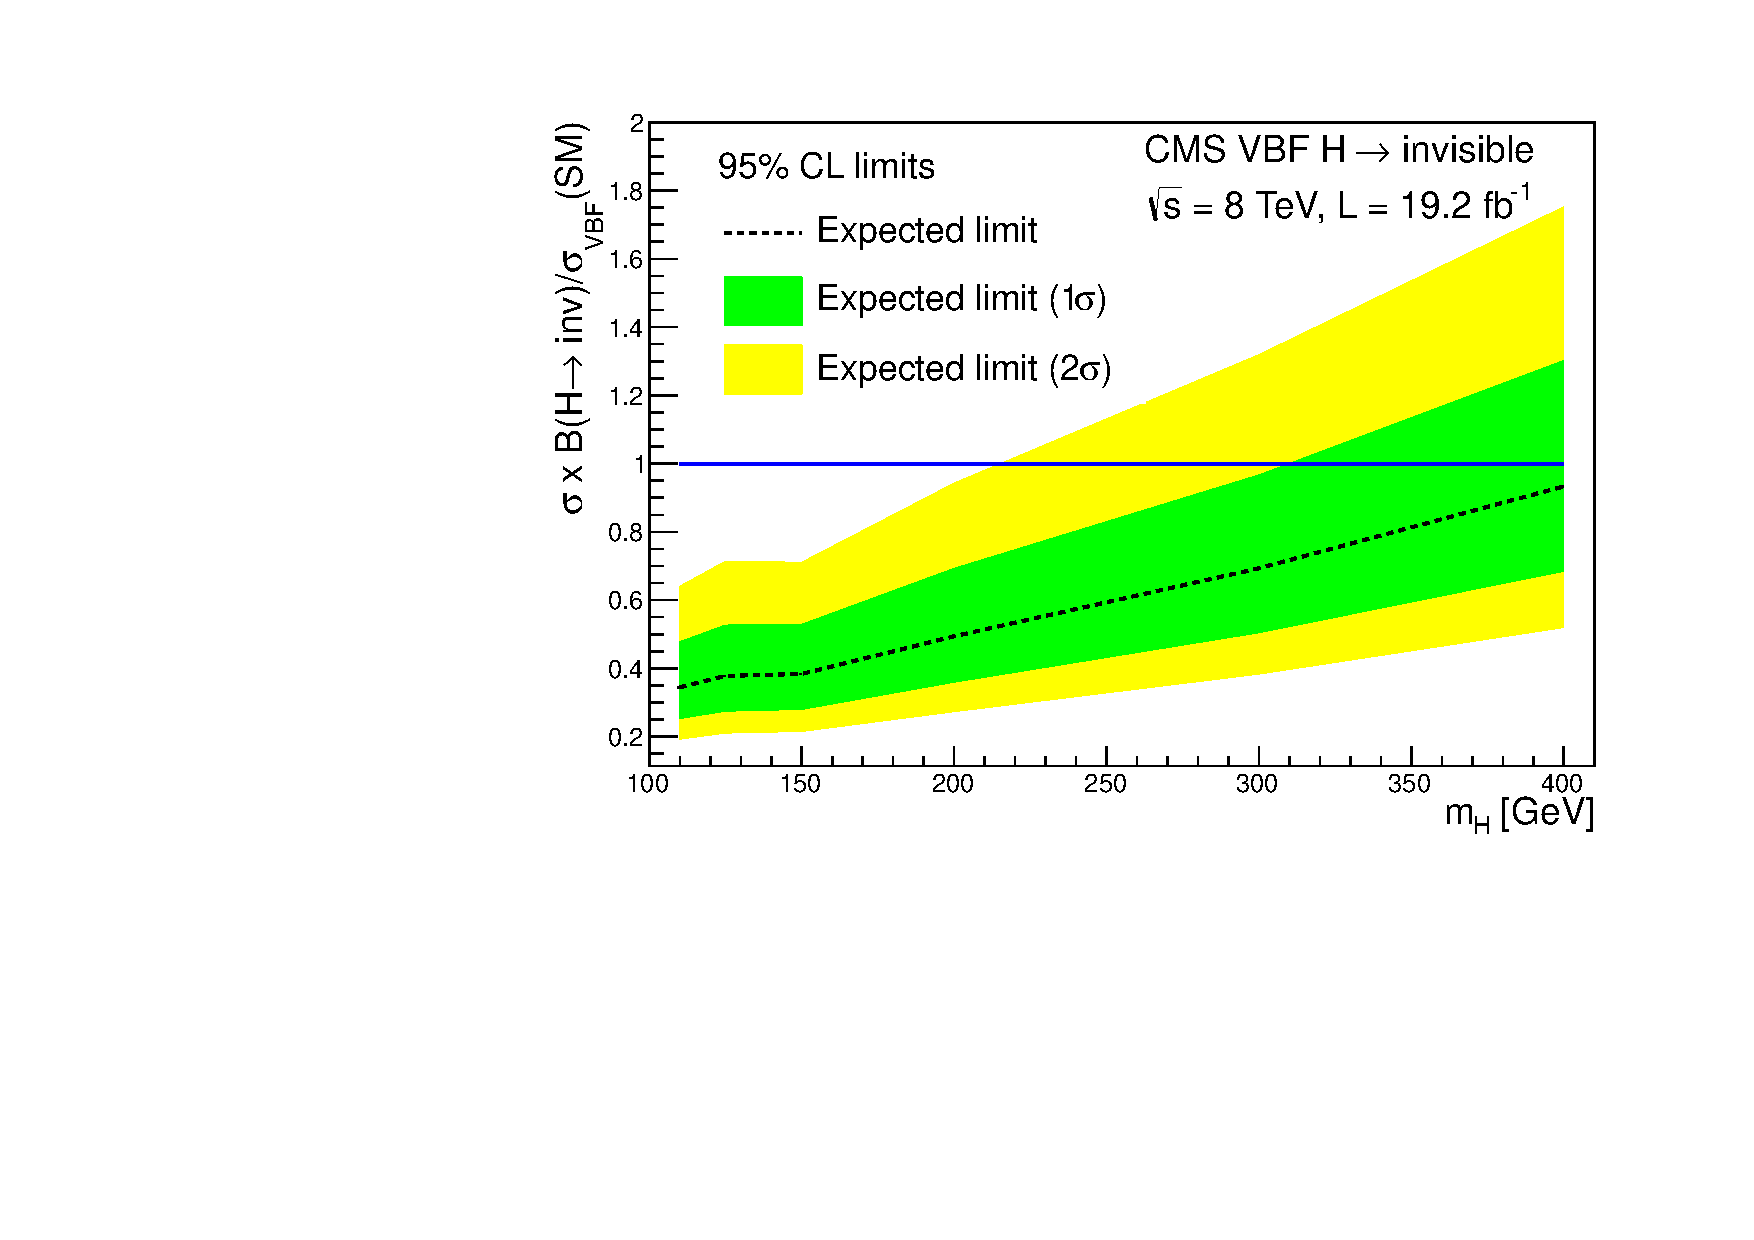
\includegraphics[width=.5\textwidth]{TalkPics/hig14038preapproval/vbflimit.pdf}
     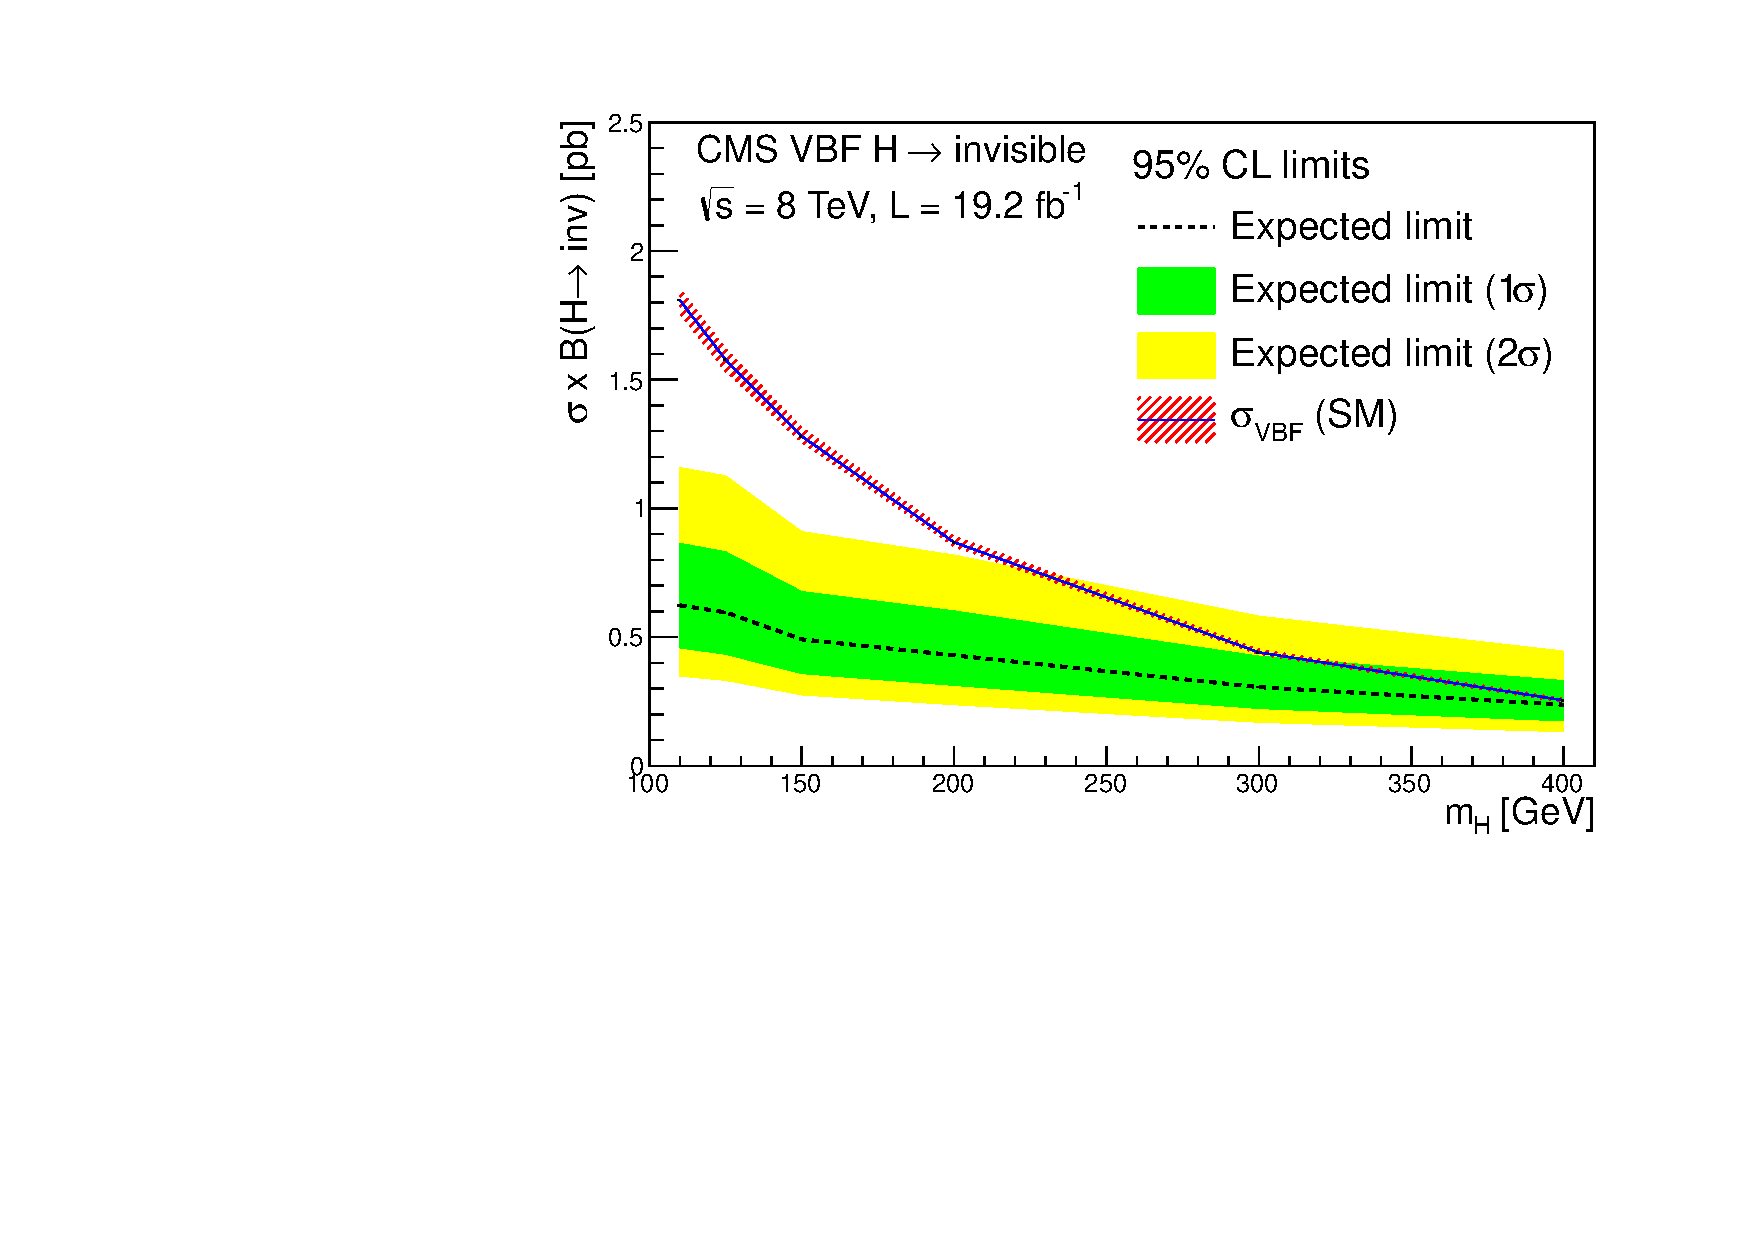
\includegraphics[width=.5\textwidth]{TalkPics/hig14038preapproval/vbfxslimit.pdf}
\end{frame}

\begin{frame}
  \frametitle{Run 2 Trigger}
  \vspace{-.1cm}
  \begin{block}{}
    \scriptsize
    \begin{itemize}
    \item Current studies performed for baseline 2015 menu and to be used in MC production
    \item Efficiencies are for VBF Higgs to invisible process with $m_{H}=125$ GeV
    \item Rates are calculated using minimum bias samples for L1 and full QCD for HLT
    \item Conditions used were 25ns bunch spacing and PU40
    \end{itemize}
  \end{block}
  \vspace{-.2cm}
  \begin{block}{\scriptsize L1}
    \scriptsize
    \begin{itemize}
    \item Start from baseline L1\_ETM70 which is planned to be in trigger menu
    \item[-] find 7 kHz individual rate, 28\% efficiency
    \item[-] run 1 ETM40 was 3kHz
    \item Systematic scan through other variables also finds:
    \item[1)] Dijet30 + fwd/bck + $\Delta\eta$(jj) $>$ 3.5 + Jet96 
    \item[-] 4.6 kHz individual rate, 21\% increase in efficiency over ETM70
    \item[2)] Dijet30 + fwd/bck + $\Delta\eta$(jj) $>$ 3.5 + ETM50 
    \item[-] 5.0 kHz individual rate, 14\% increase in efficiency over ETM70
    \end{itemize}
  \end{block}
\end{frame}

\begin{frame}
  \frametitle{Run 2 Trigger}
  \begin{block}{\scriptsize HLT}
    \scriptsize
    \begin{itemize}
    \item Use L1\_ETM70 as seed
    \item Baseline HLT path in menu is HLT\_PFMET170\_NoiseCleaned with 9\% efficiency
    \item Scan over variables also finds:
    \item[-] HLT\_DiPFJetVBF40\_DEta3p5\_MJJ600\_PFMETNoMu140
    \item[-] Additional rate 4.7 Hz total efficiency 10.5\%
    \item We also proposed a prescaled control trigger for efficiency measurements:
    \item[-] HLT\_DiPFJetVBF40\_DEta3p5\_MJJ600\_PFMETNoMu80 seeded by L1\_ETM50 with rate 0.5 Hz
    \end{itemize}
  \end{block}
  \begin{block}{}
    \scriptsize
    \begin{itemize}
    \item For comparison run 1 prompt trigger had 8\% efficiency at HLT for 1 Hz
    \end{itemize}
  \end{block}
\end{frame}

\setbeamercolor{background canvas}{bg=}

\includepdf[pages=8]{TalkPics/cmsuk0115/VBFHInv_Trig2015_27Oct2015.pdf}

\begin{frame}
  \frametitle{Summary}
  \label{lastframe}
  \vspace{-.3cm}
  \begin{block}{}
    \scriptsize
    \begin{itemize}
    \item New cut based analysis presented with less QCD and higher signal efficiency
    \item[-] Made possible by looser parked trigger thresholds
    \item[-] Expected limit {\color{red}38\%} improved from 49\% for prompt analysis
    \item This analysis will be used as our baseline for run 2 studies
    \item Run 2 trigger plans shown
    \item[-] We can match/improve on run 1 efficiency
    \item[-] Offline studies to follow
    \end{itemize}
  \end{block}
  \vspace{-.1cm}
     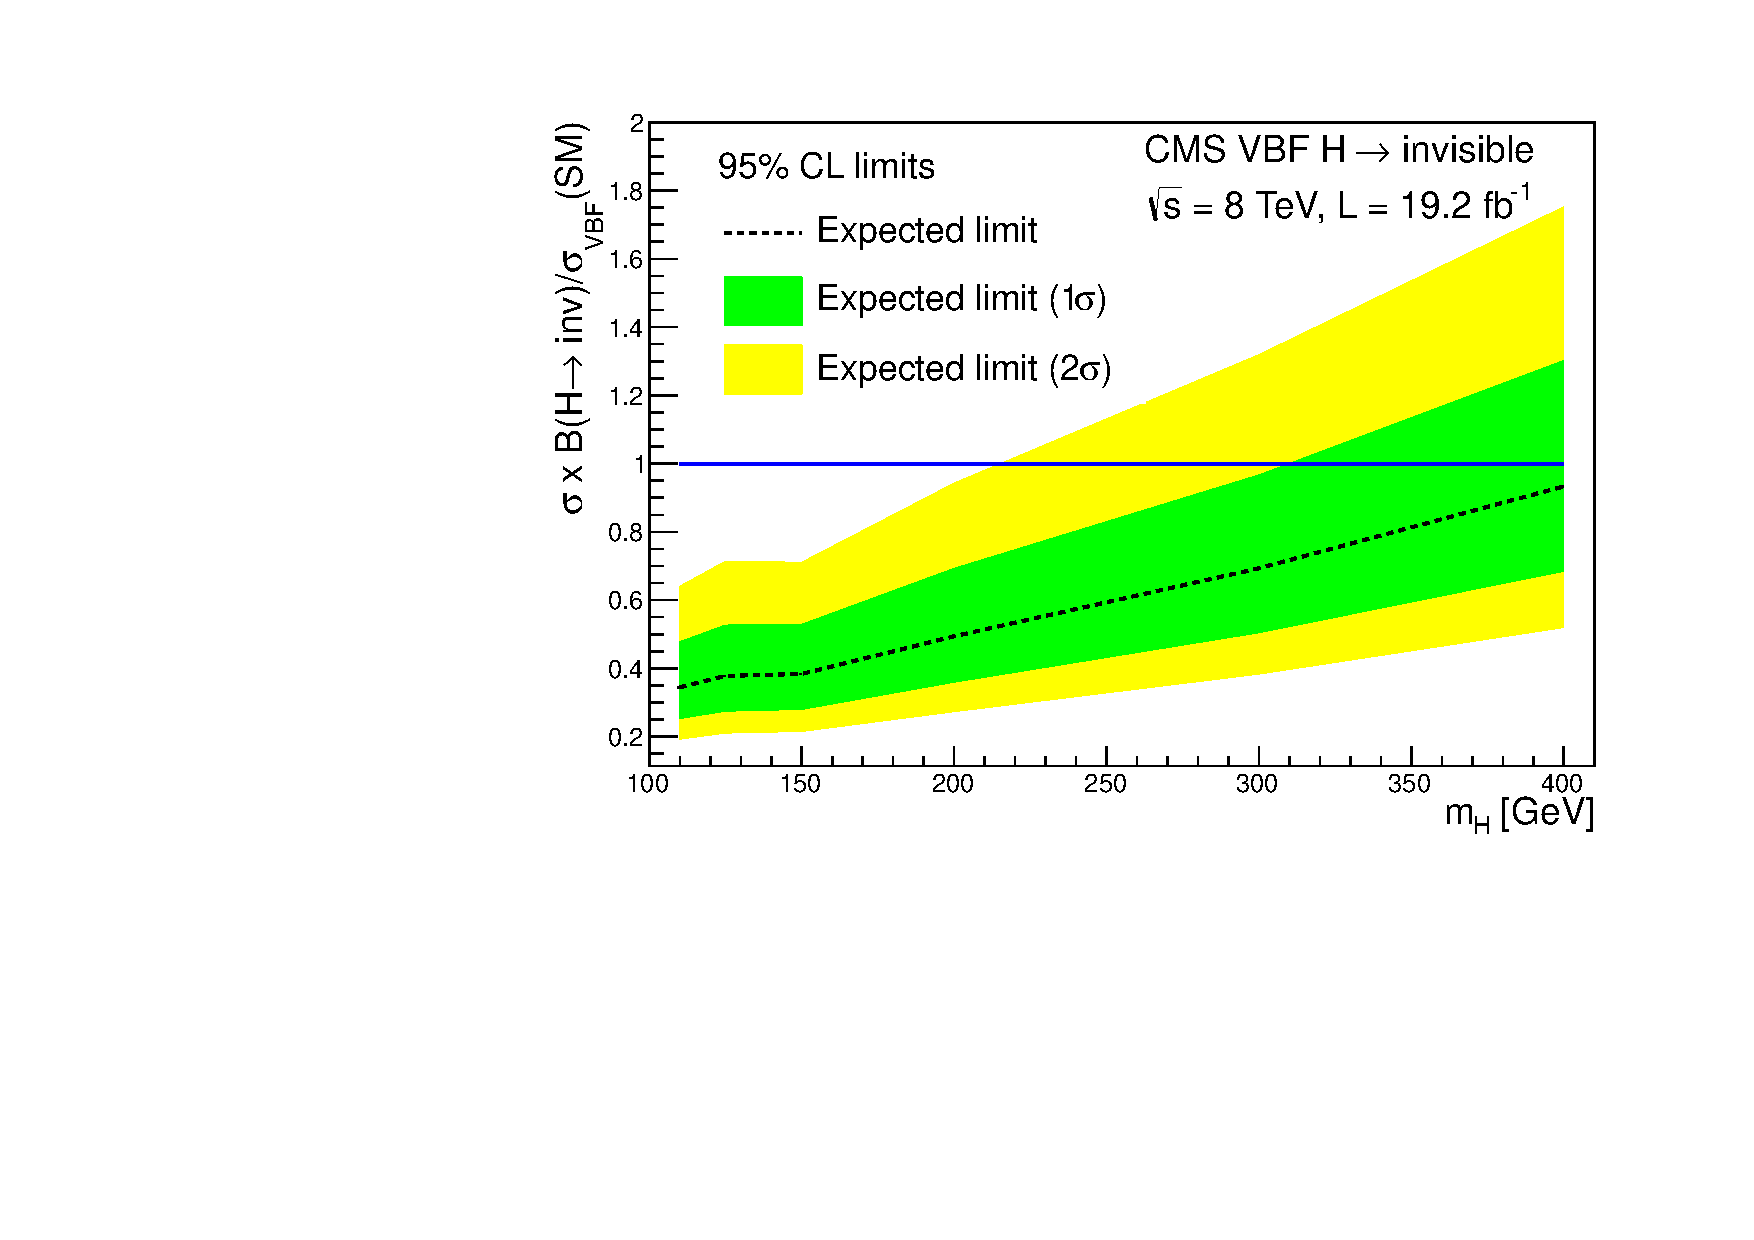
\includegraphics[clip=true,trim=0 0 0 20,width=.5\textwidth]{TalkPics/hig14038preapproval/vbflimit.pdf}
     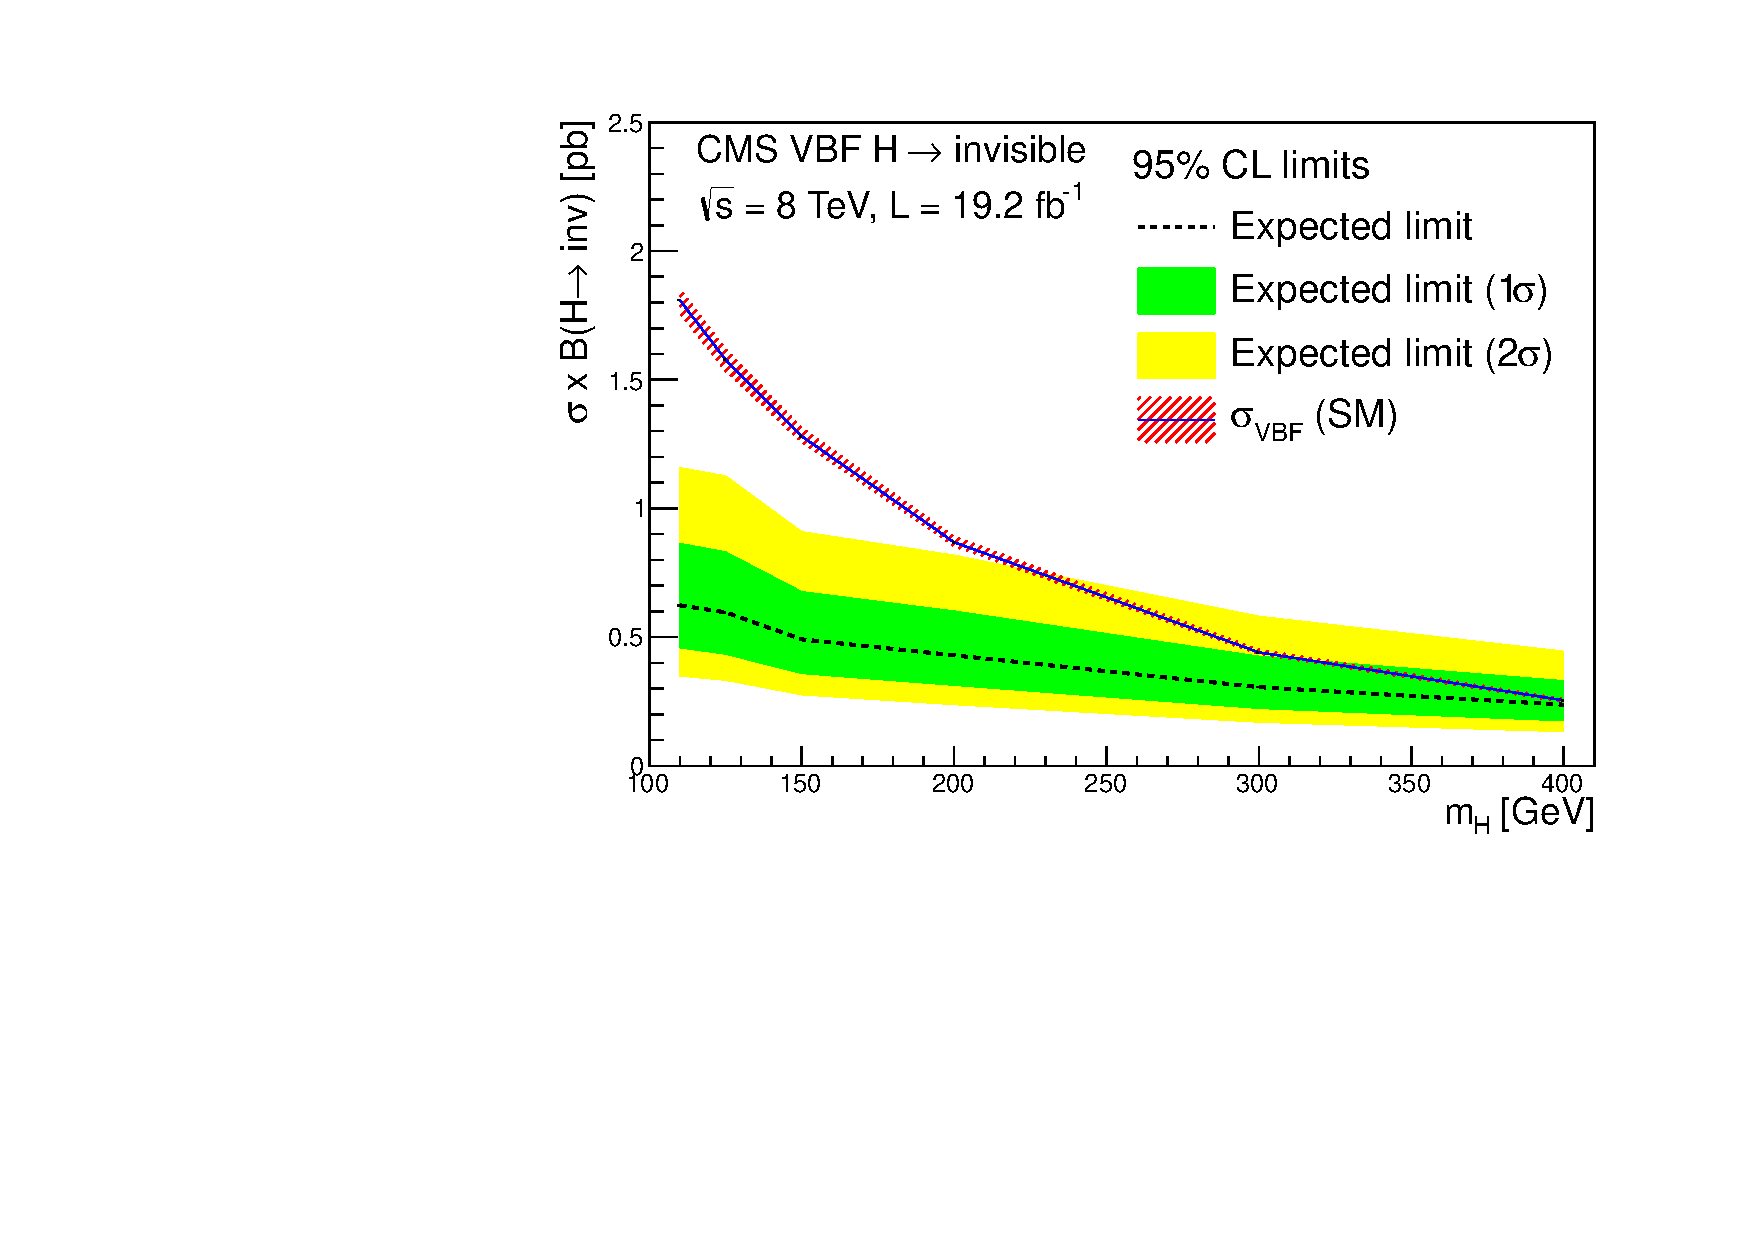
\includegraphics[clip=true,trim=0 0 0 20,width=.5\textwidth]{TalkPics/hig14038preapproval/vbfxslimit.pdf}
\end{frame}

%UPDATED BACKUP
\begin{frame}
  \frametitle{Backup}
\end{frame}


%DOCUMENTATION
\begin{frame}
  \frametitle{Documentation}
  \begin{columns}
    \column{.5\textwidth}
    AN-14-243
    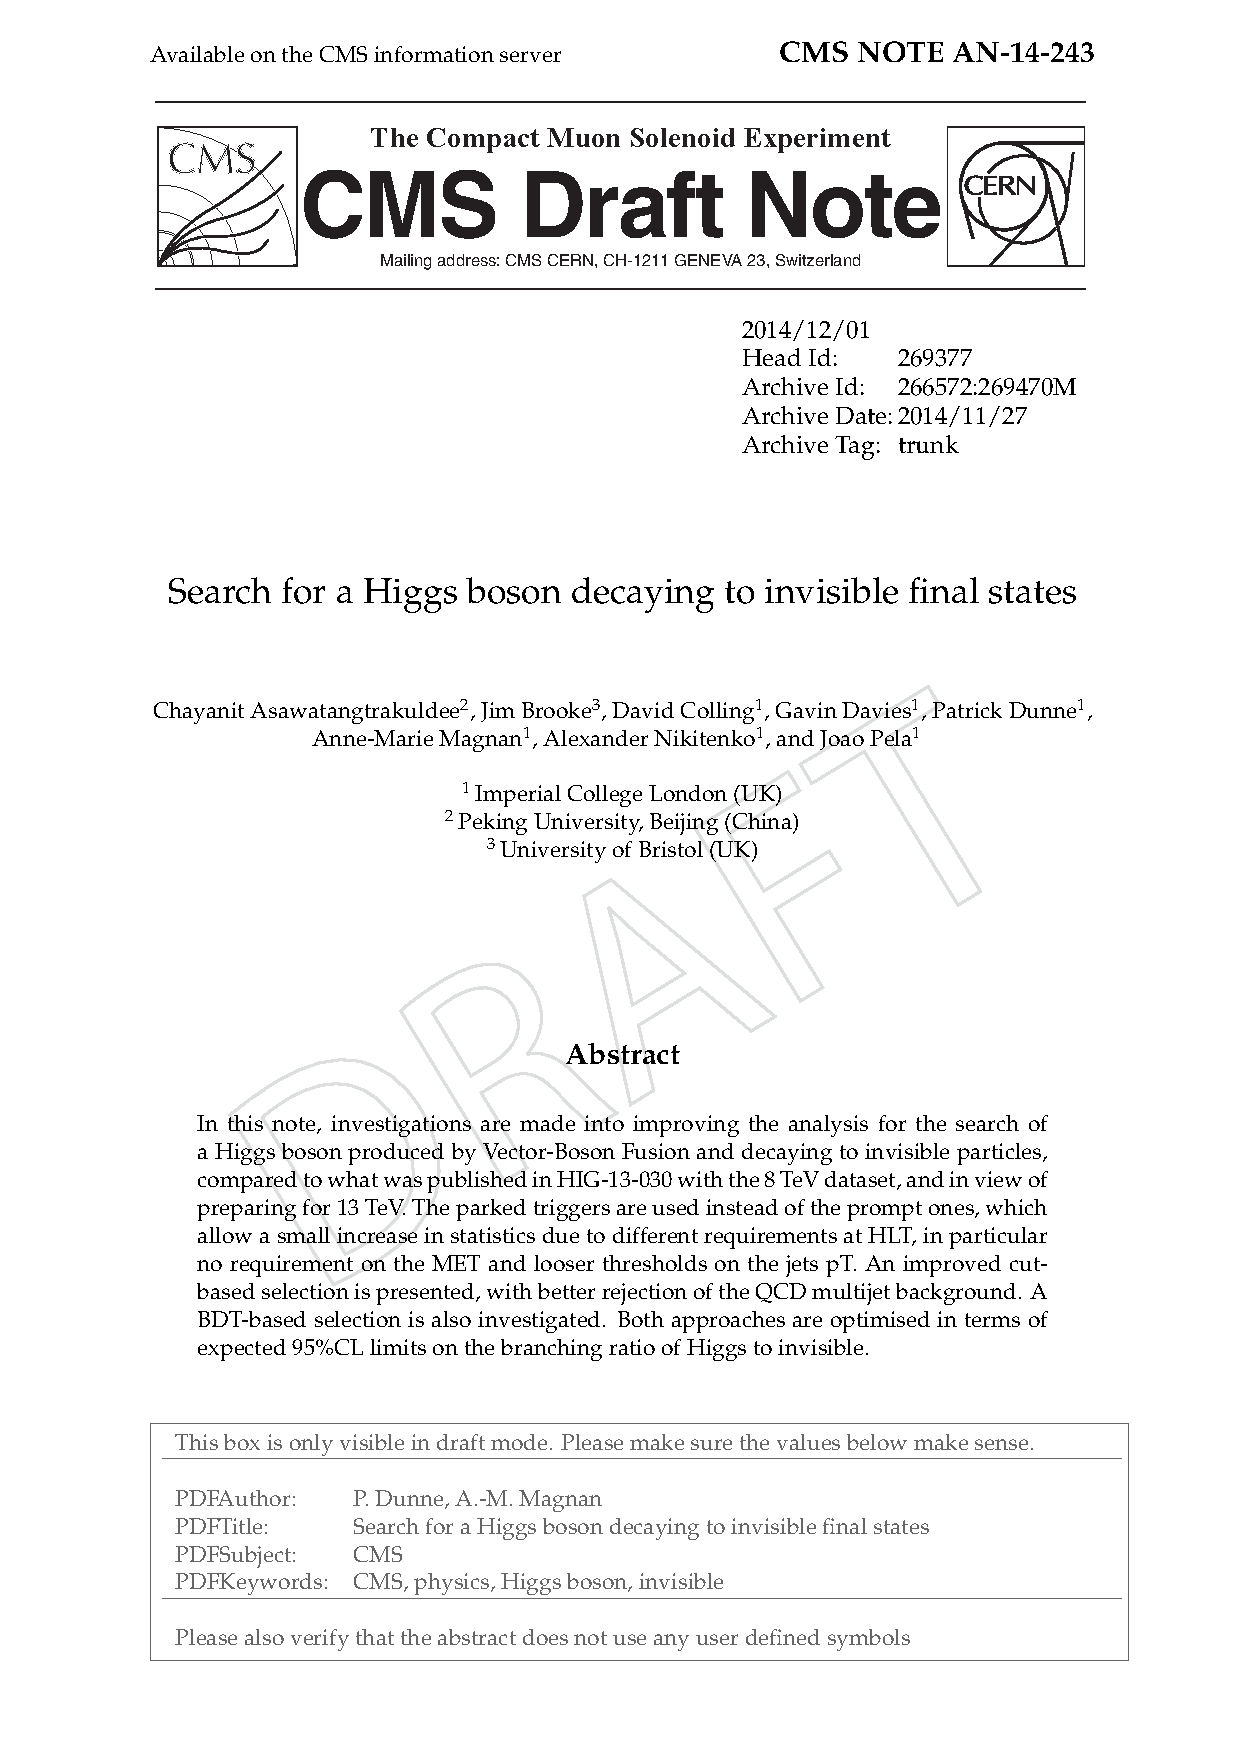
\includegraphics[width=.85\textwidth,page=1]{TalkPics/hig14038preapproval/AN2014_243_v6.pdf}
    \column{.5\textwidth}
    HIG-14-038
    
\includegraphics[width=.85\textwidth,page=1]{TalkPics/hig14038preapproval/HIG-14-038-pas-v0.pdf}
  \end{columns}
\end{frame}

%THEORY MOTIVATION
\begin{frame}
    \frametitle{Why Higgs to Invisible?}
    \label{motivation}
    \vspace{-.2cm}
    \begin{columns}
      \column{.5\textwidth}
      \begin{block}{\scriptsize Experimental motivation}
        \scriptsize
        \begin{itemize}
        \item Current measurements of the 125 GeV Higgs boson are compatible with Standard Model (SM) expectations
        \item[-] large uncertainties can still accommodate significant beyond the SM (BSM) properties
        \item Additional Higgs bosons with exotic decays are not excluded
        \end{itemize}
      \end{block}
      \column{.45\textwidth}
      \hfill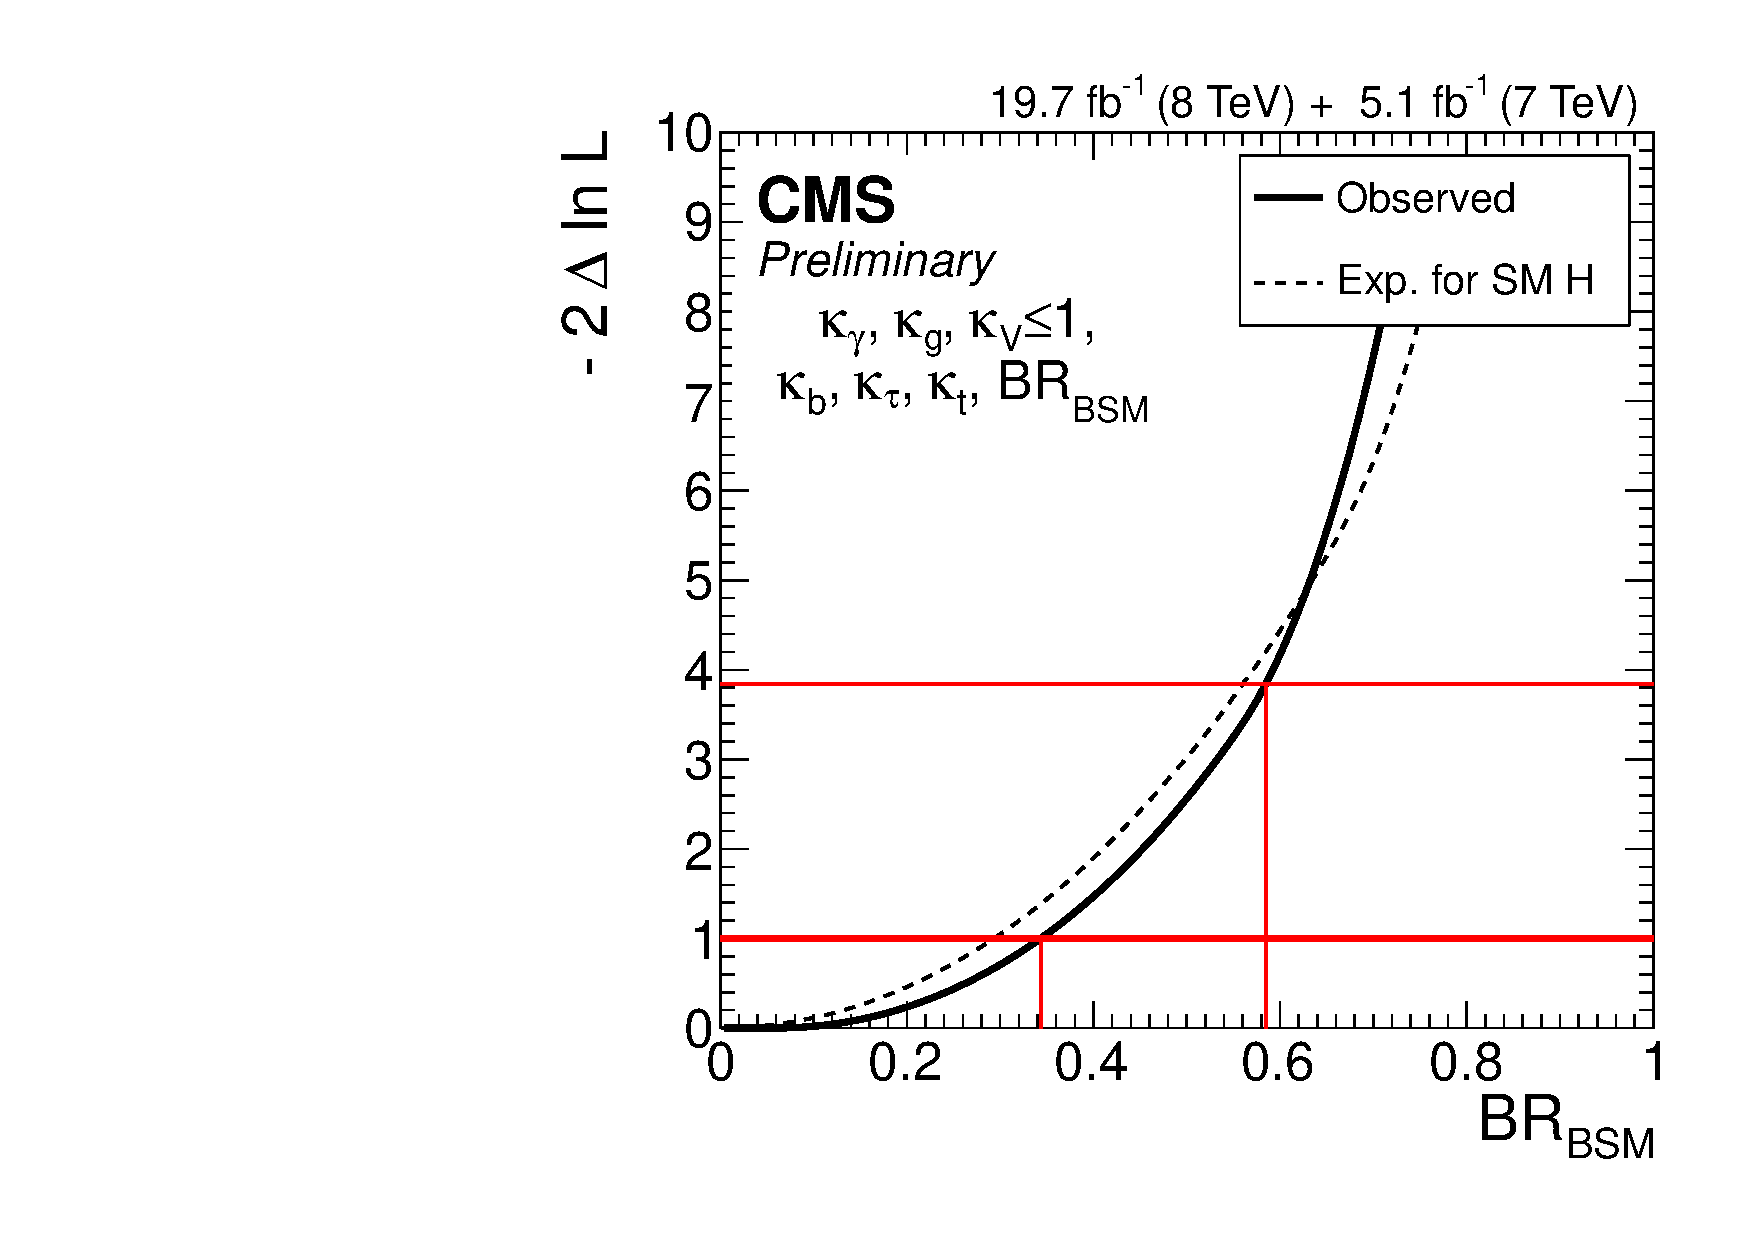
\includegraphics[height=.55\textheight]{TalkPics/panicpics/indirectbrbsm.pdf}
      \column{.05\textwidth}
    \end{columns}
    \begin{columns}
      \column{1.095\textwidth}
      \begin{block}{\scriptsize Theoretical motivation}
        \scriptsize
        \begin{itemize}
        \item Many BSM theories predict Higgs boson decays to invisible final states:
        \item[-] e.g. SUSY, extra dimensions, fourth-generation neutrinos
        \item These final state particles are often dark matter candidates
        \end{itemize}
      \end{block}
    \end{columns}

  \end{frame}

\begin{frame}
  \frametitle{Parked Triggers}
  \vspace{-.2cm}
  \begin{block}{}
      \scriptsize
    \begin{itemize}
    \item Use already analysed prompt trigger for run A
    \item One parked trigger for runs B and C, another for run D
    \item[-] Parked trigger cuts are looser so prompt trigger not used where parked trigger is available
    \item All parked and prompt triggers are seeded by L1\_ETM40
    \item Parked triggers have looser HLT thresholds
    \item This allows us to look at new regions of phase space and different analysis techniques
    \item Use prompt analysis as a base:
    \item[-] e.g. same objects and MC samples
    \end{itemize}
  \end{block}
  \vspace{-.2cm}
  \begin{block}{\scriptsize HLT}
    \scriptsize
    \centering
    \begin{tabular}{|l|c|c|c|}
      \hline
      Run period & MET cut & dijet $p_{T}$ cut & dijet mass cut \\
      \hline
      A & METnoMuons$>$65 GeV & DiPFJet40 & MJJ800 \\
      B\&C & N/A & DiJet35 & MJJ700 \\
      D & N/A & DiJet30 & MJJ700 \\
      \hline
    \end{tabular}
  \end{block}
\end{frame}

%TRIGGER EFFICIENCY
\begin{frame}
  \frametitle{Trigger efficiency}
  \begin{columns}
    \column{.55\textwidth}
    \begin{block}{}
      \scriptsize
      \begin{itemize}
      \item Variables used in prompt and parked triggers are highly correlated:
      \item[-] dijet mass, METnoMU, jet 2 $p_{T}$
      \item In the prompt analysis correlations were neglected  as we cut to ensure trigger was $>95\%$ efficient
      \item For the parked analysis we use a 2D binning in dijet mass and jet 2 $p_{T}$
      \item[-] MJJ: 0,600,800,900,1000,5000
      \item[-] Jet 2 $p_{T}$: 30,40,50,60,1000
      \item In each bin we fit the METnoMU trigger turn on using an error function
      \item We then combine the turn ons from runs A, BC and D weighted by luminosity and apply this to MC events

      \end{itemize}
    \end{block}
    \column{.5\textwidth}
    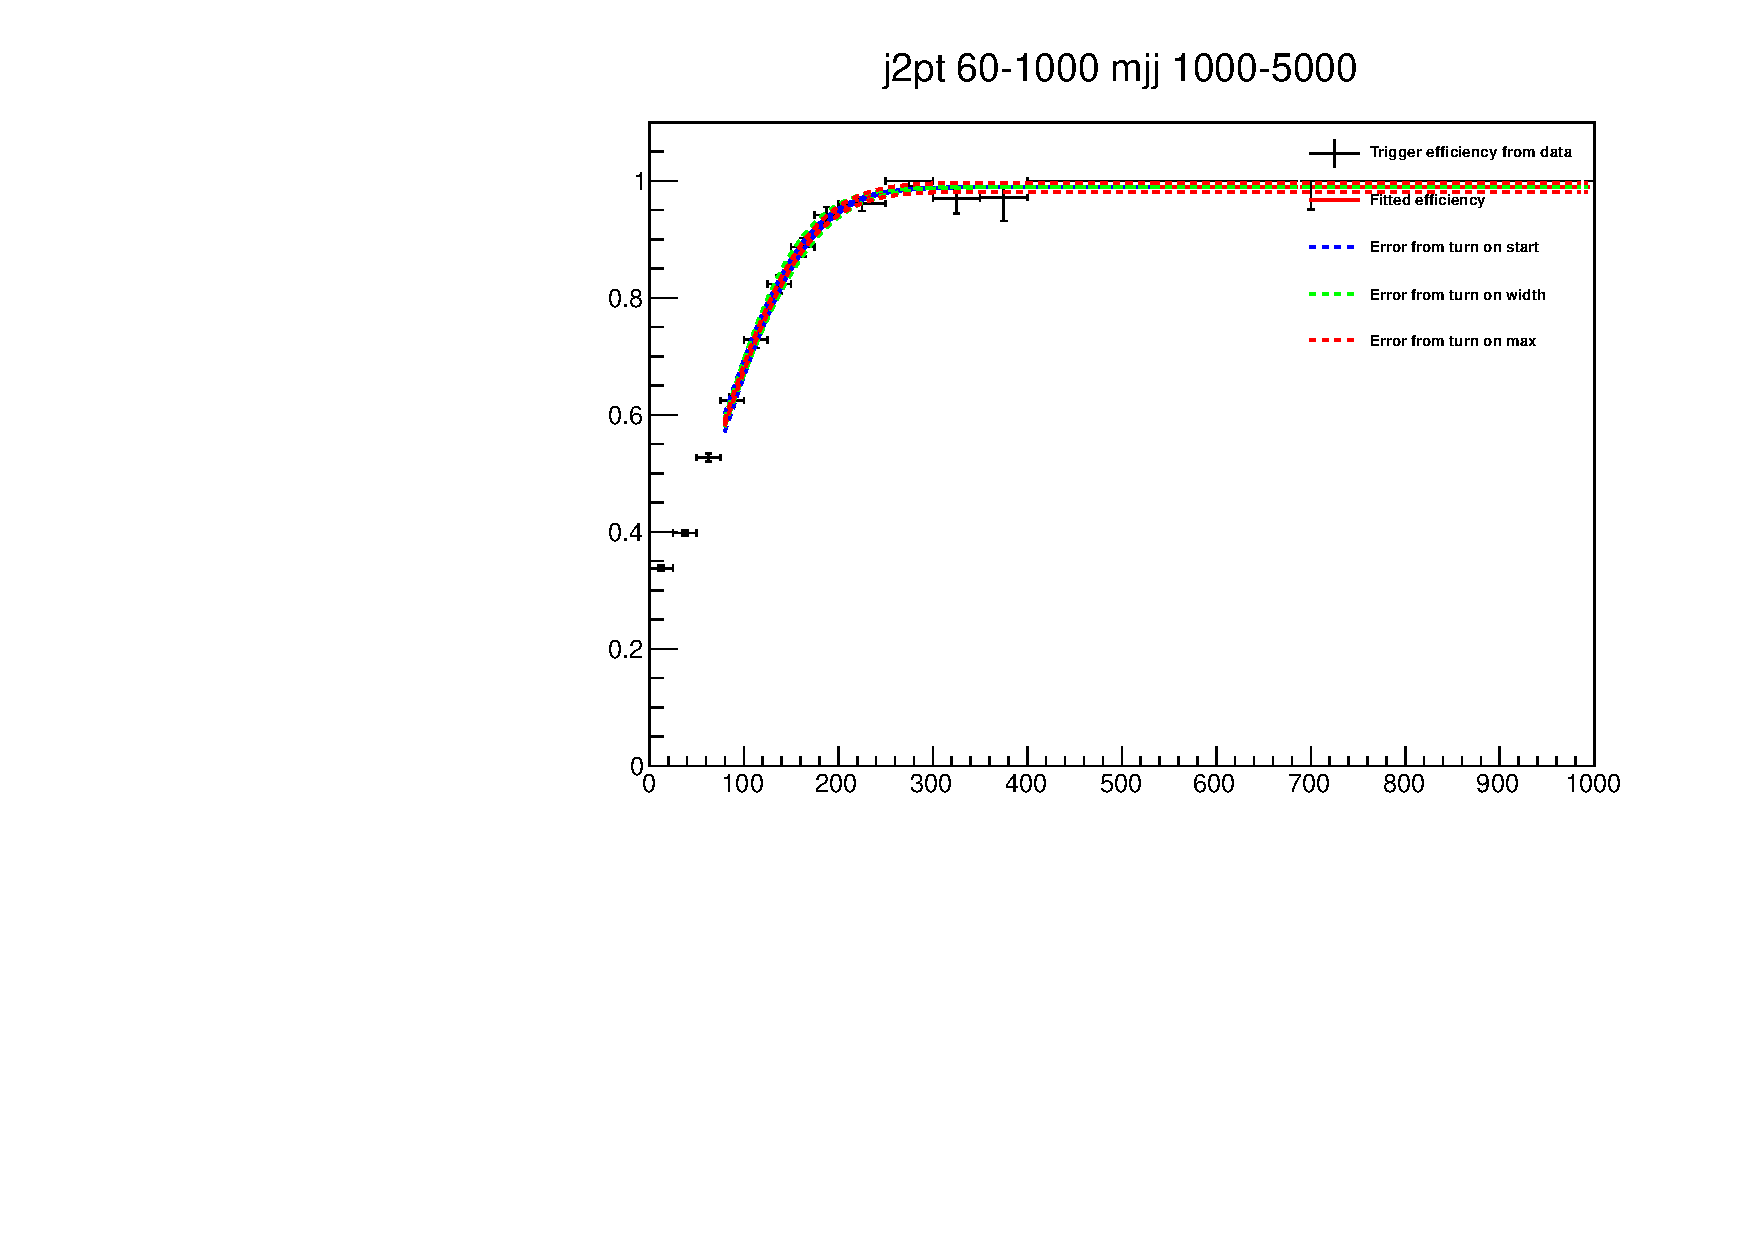
\includegraphics[width=1.1\textwidth]{TalkPics/hig14038preapproval/trigfitplots/hData_MET_1D_45D.pdf}
    \vspace{-.2cm}

    \hfill \scriptsize METnoMU/GeV
  \end{columns}
\end{frame}

\begin{frame}
  \frametitle{Prompt vs Parked selection}
  \begin{block}{}
    \scriptsize
    \begin{itemize}
    \item Summary of differences in signal region selection
    \end{itemize}
    \centering
    \begin{tabular}{|l|c|c|}
      \hline
      Variable & Prompt cut & Parked cut \\
      \hline
      \hline
      Lepton veto & \multicolumn{2}{|c|}{no veto e or $\mu$} \\
      \hline
      $\eta_{j1,2}$ & \multicolumn{2}{|c|}{$<4.7$} \\
      \hline
      $\eta_{j1}\cdot\eta_{j2}$ & \multicolumn{2}{|c|}{$<0$} \\
      \hline
      jet 1 $p_{T}$ & \multicolumn{2}{|c|}{$>50$ GeV} \\
      \hline
      jet 2 $p_{T}$ & $>50$ GeV & $>45$ GeV \\
      \hline
      $\Delta\eta_{jj}$ & $>4.2$ & $>3.6$ \\
      \hline
      $M_{jj}$ & $>1100$ GeV & $>1200$ GeV \\
      \hline
      $\text{METnomu}$& $>130$ GeV &$>90$ GeV \\
      \hline
      Central jet veto & yes & no \\
      \hline
      $\Delta\phi_{jj}$ & $<1.0$ & no cut \\
      \hline
      $\frac{METnoMU}{\sigma_{METnoMU}}$& no cut & $>4$ \\
      \hline
      $\text{Min}\Delta\phi(all\,jets,METnomu)$& no cut &$>2.3$ \\
      \hline
    \end{tabular}
  \end{block}
\end{frame}

\begin{frame}
  \frametitle{$W\rightarrow e\nu$}
  \vspace{-.2cm}
  \begin{block}{}
    \scriptsize
    \begin{itemize}
      \vspace{-.1cm}
    \item Data-MC agreement good
      \vspace{-.1cm}
    \item Same method used as for prompt analysis
    \end{itemize}
    \vspace{-.2cm}
    \centering
    \begin{tabular}{|l|c|c|}
      \hline
      & Signal region & Control region \\
      \hline
      N$^{data}$&XXX&$68\pm 8.2$(stat.)\\
      N$^{bkg}$&N/A&$3.1\pm 1.5$(stat.)\\
      N$^{W MC}$&$114.6\pm8.9$(stat.)&$129.6\pm 8.1$(stat.)\\
      \hline
      $(N^{data}-N^{bkg})/N^{W MC}_{C}$ & \multicolumn{2}{|c|}{$0.50\pm0.06$(stat.)$\pm0.03$(MC stat.)} \\
      \hline
      Final estimate&\textcolor{red}{$57.4\pm7.3$(stat.)$\pm5.9$(MC stat.)}&N/A \\
      \hline
    \end{tabular}

  \end{block}

  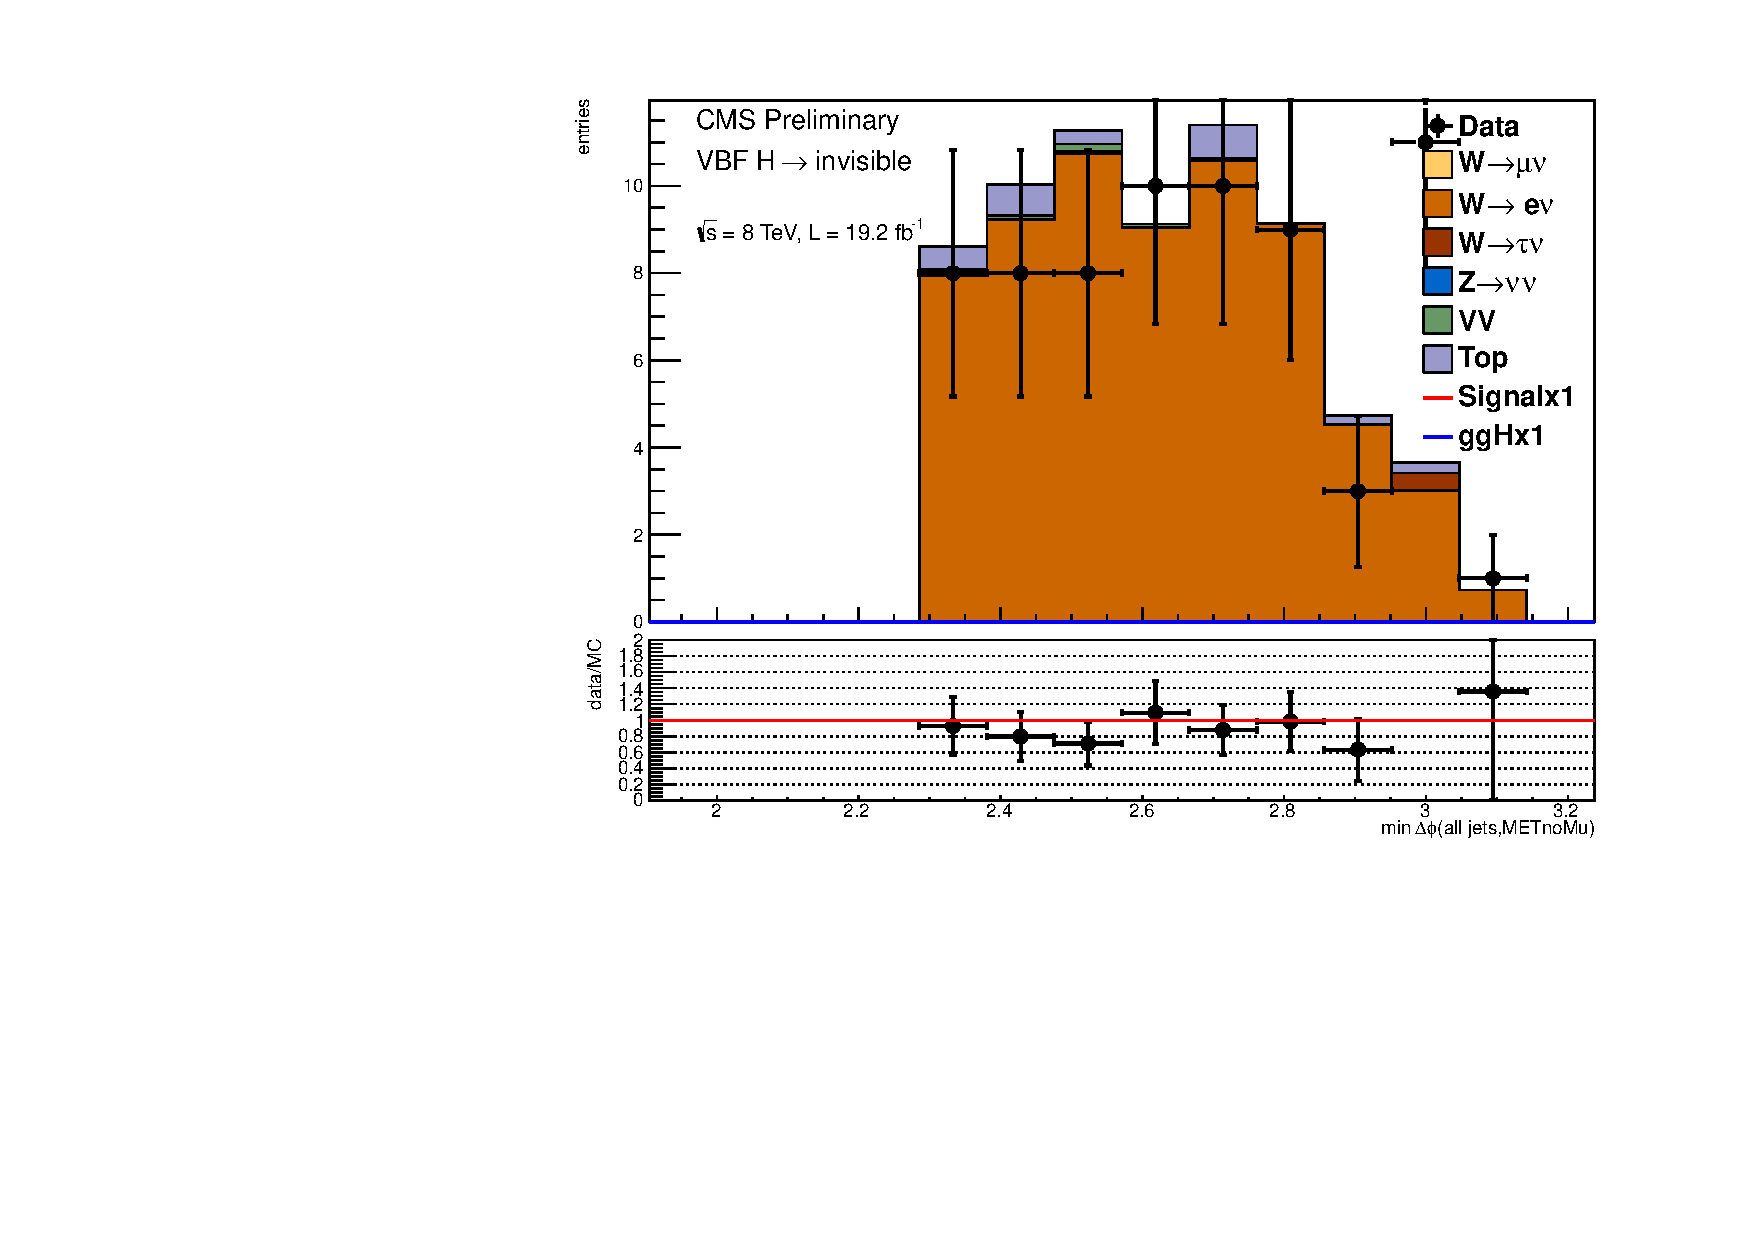
\includegraphics[clip=true,trim= 0 0 0 20,width=.5\textwidth]{TalkPics/hig14038preapproval/output_sigreg/enu_alljetsmetnomu_mindphi}
  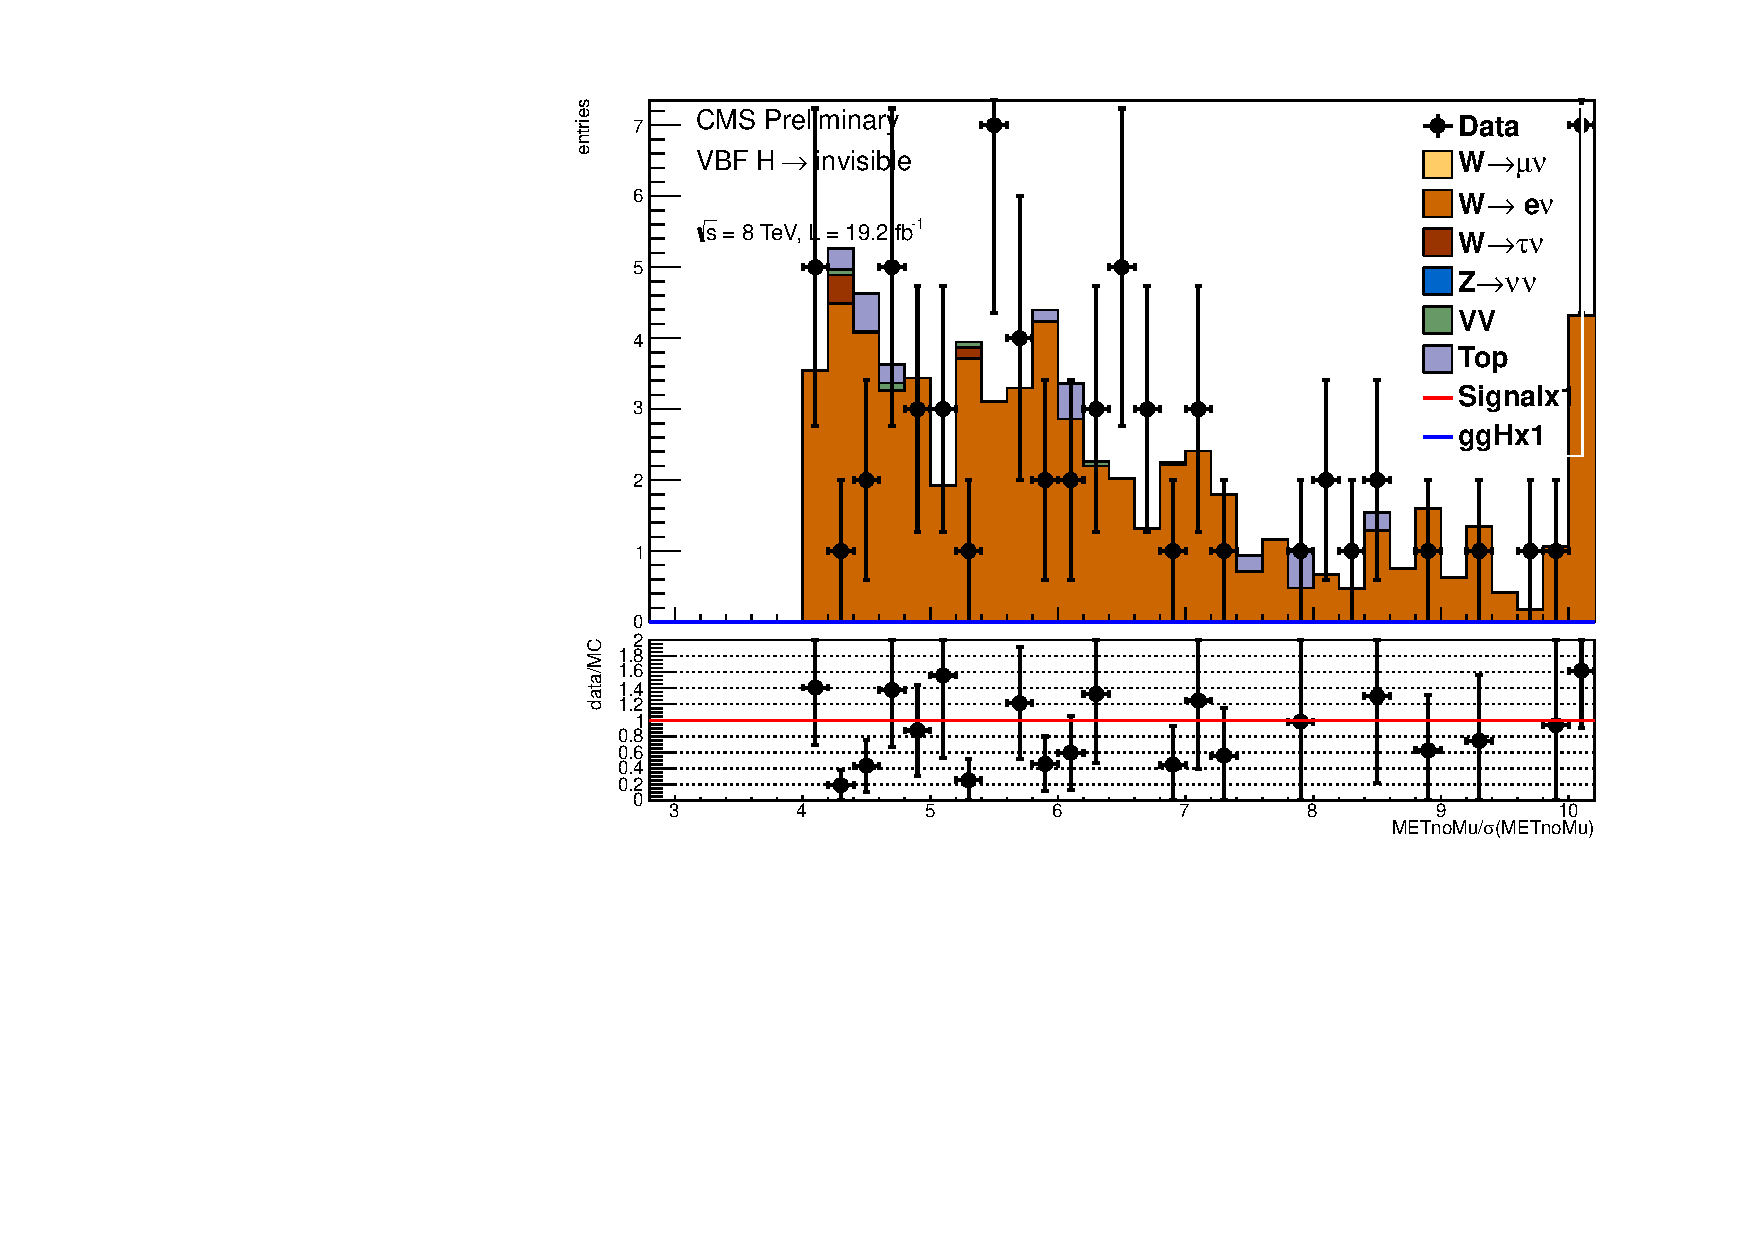
\includegraphics[clip=true,trim=0 0 0 20,width=.5\textwidth]{TalkPics/hig14038preapproval/output_sigreg/enu_metnomu_significance}
  
\end{frame}

\begin{frame}
  \frametitle{$W\rightarrow \mu\nu$}
  \vspace{-.3cm}
  \begin{block}{}
    \scriptsize
    \begin{itemize}
\vspace{-.1cm}
    \item Data-MC agreement good
\vspace{-.1cm}
    \item Same method used as for prompt analysis
    \end{itemize}
\vspace{-.2cm}
\centering
    \begin{tabular}{|l|c|c|}
\hline
 & Signal region & Control region \\
\hline
N$^{data}$&XXX&$300\pm 17.3$(stat.)\\
N$^{bkg}$&N/A&$12.7\pm 4.6$(stat.)\\
N$^{W MC}$&$142.1\pm10.1$(stat.)&$401.1\pm 15.1$(stat.)\\
\hline
$(N^{data}-N^{bkg})/N^{MC}_{C}$ & \multicolumn{2}{|c|}{$0.72\pm0.04$(stat.)$\pm0.03$(MC stat.)} \\
\hline
Final estimate&\textcolor{red}{$101.8\pm6.1$(stat.)$\pm8.3$(MC stat.)}&N/A \\
\hline
\end{tabular}
  \end{block}
  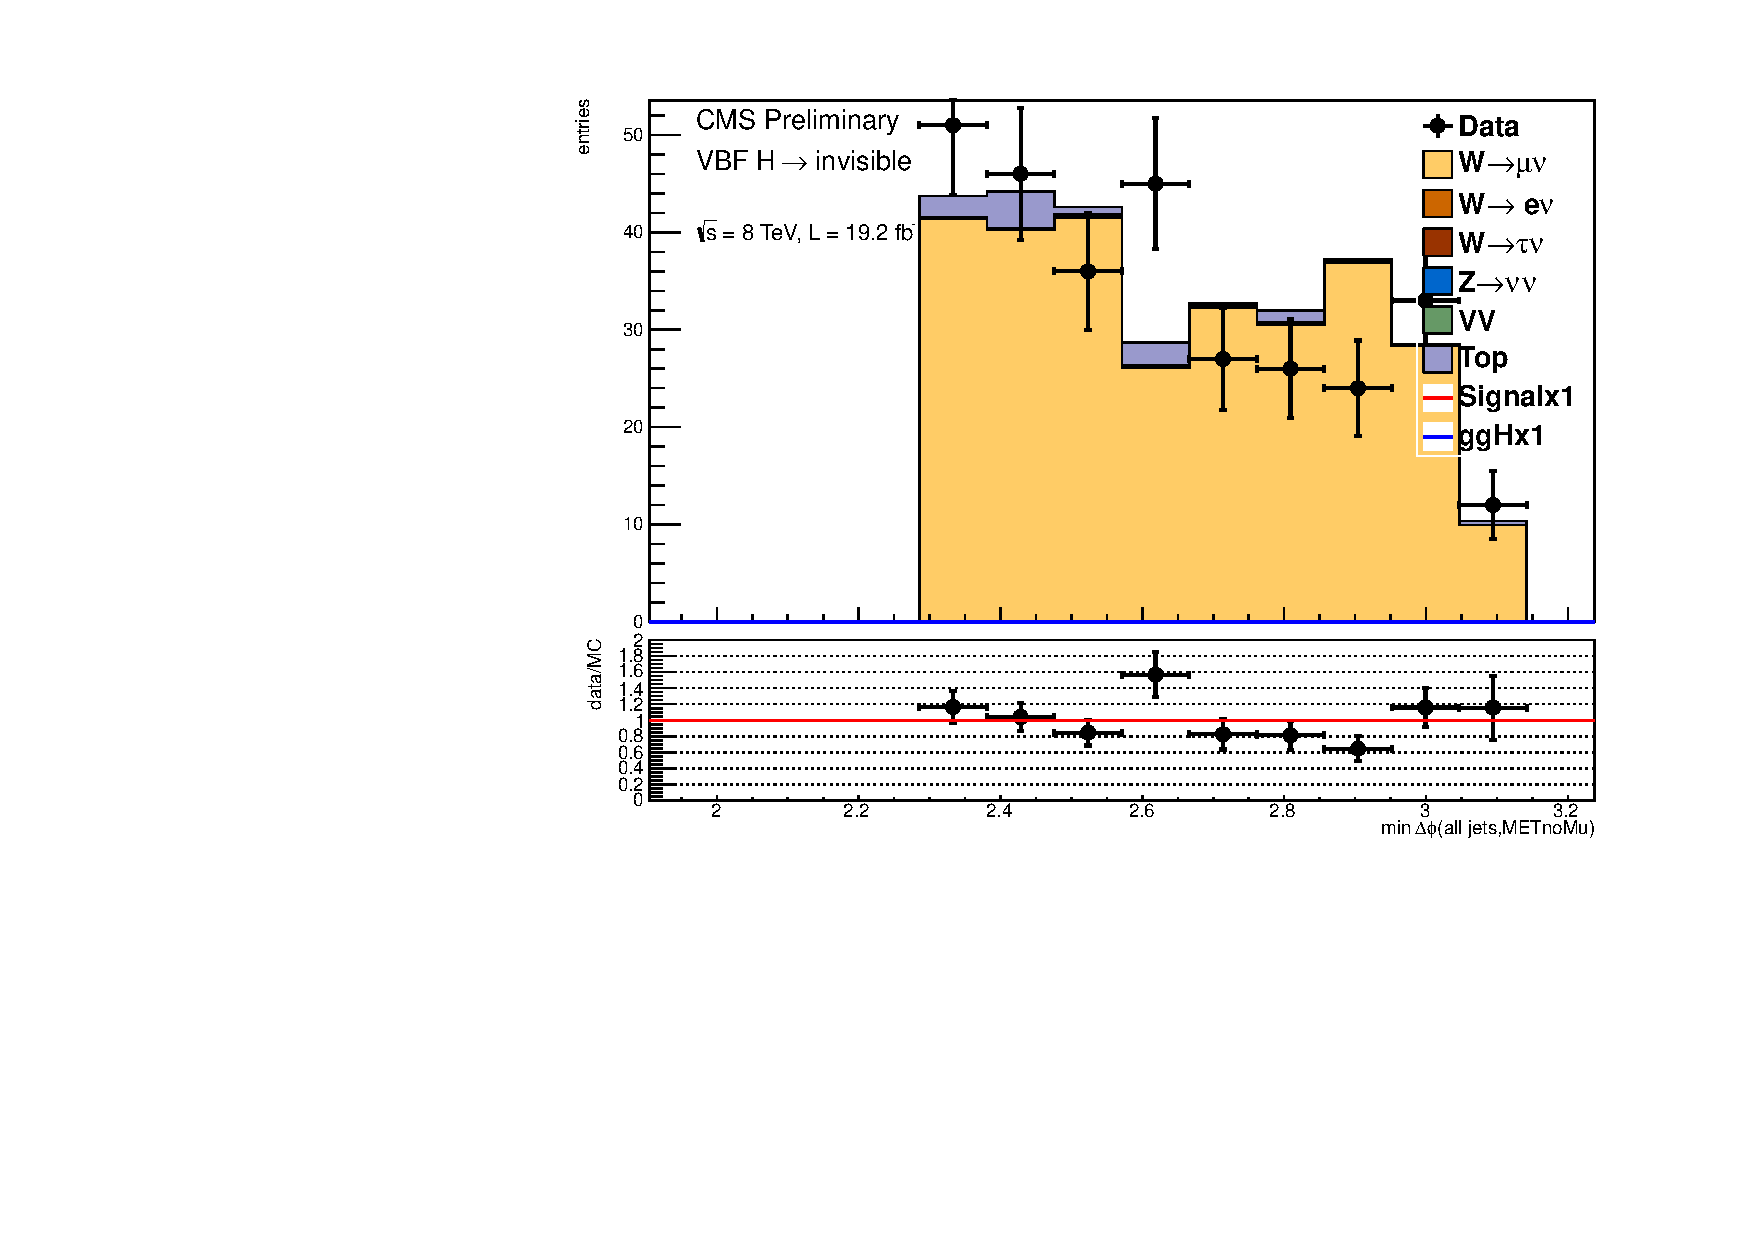
\includegraphics[clip=true, trim = 0 0 0 20,width=.5\textwidth]{TalkPics/hig14038preapproval/output_sigreg/munu_alljetsmetnomu_mindphi}
  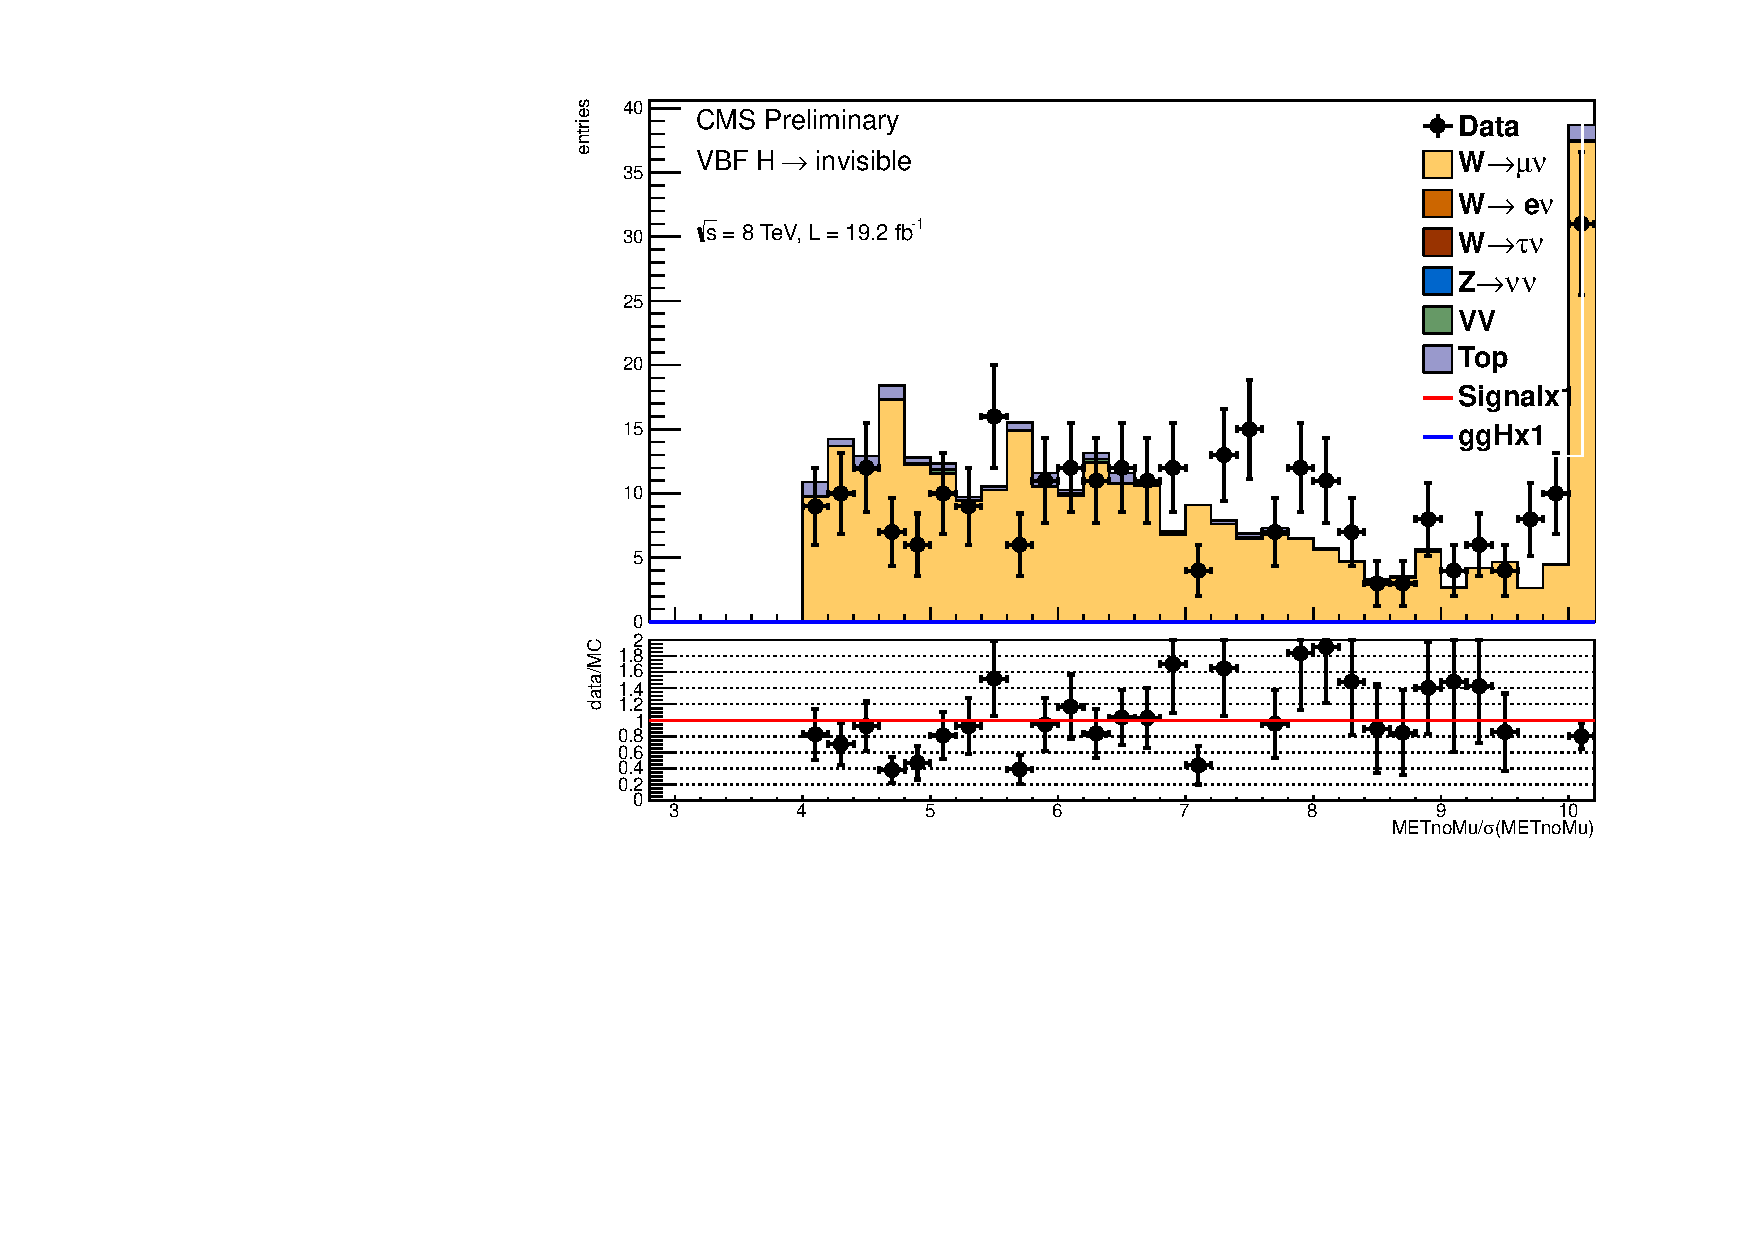
\includegraphics[clip=true, trim = 0 0 0 20,width=.5\textwidth]{TalkPics/hig14038preapproval/output_sigreg/munu_metnomu_significance}
\end{frame}

\begin{frame}
  \frametitle{$W\rightarrow\tau\nu$ control region}
  \begin{columns}
    \column{1.08\textwidth}
  \begin{columns}
    \column{.55\textwidth}
    \vspace{-.3cm}
    
    \begin{block}{}
      \scriptsize
      \begin{itemize}
      \item Difference in weight between control region and signal region cuts used to estimate error
      \item Measured in $W\rightarrow\mu\nu$ which has enough events to see data driven weight variation with $\text{Min}\Delta\phi(all\,jets,\,METnomu)$ cut 
      \item[-] weight changes by 20\% when loosening cut from 2.3 to 1.0.
      \item[-] We add a 20\% systematic on the $W\rightarrow\tau\nu$ background
      \end{itemize}
      \begin{tabular}{|l|c|c|}
        \hline
        $N_{C}^{data}$ & $76 \pm 8.7  (stat.)$\\
        $N_{C}^{bkg}$ & $11.3 \pm 4.6 (MC stat.)$  \\
        $N_{S}^{MC}$ & $122.6\pm 8.8  (MC stat.)$ \\
        $N_{C}^{MC}$ & $81.0 \pm 6.4 (MC stat.)$   \\
        \hline
        \tiny $\frac{N^{data}-N^{bkg}}{N^{MC}_{C}}$ & \scriptsize $0.80\pm0.11$(stat.)$\pm0.08$(MC stat.) \\
        \hline
        $N_{S}^{W}$ & \textcolor{red}{$98.0 \pm 13.2 (stat.) \pm 12.6 (MC stat.)$}  \\ 
        \hline
      \end{tabular}
    \end{block}
    \column{.46\textwidth}
    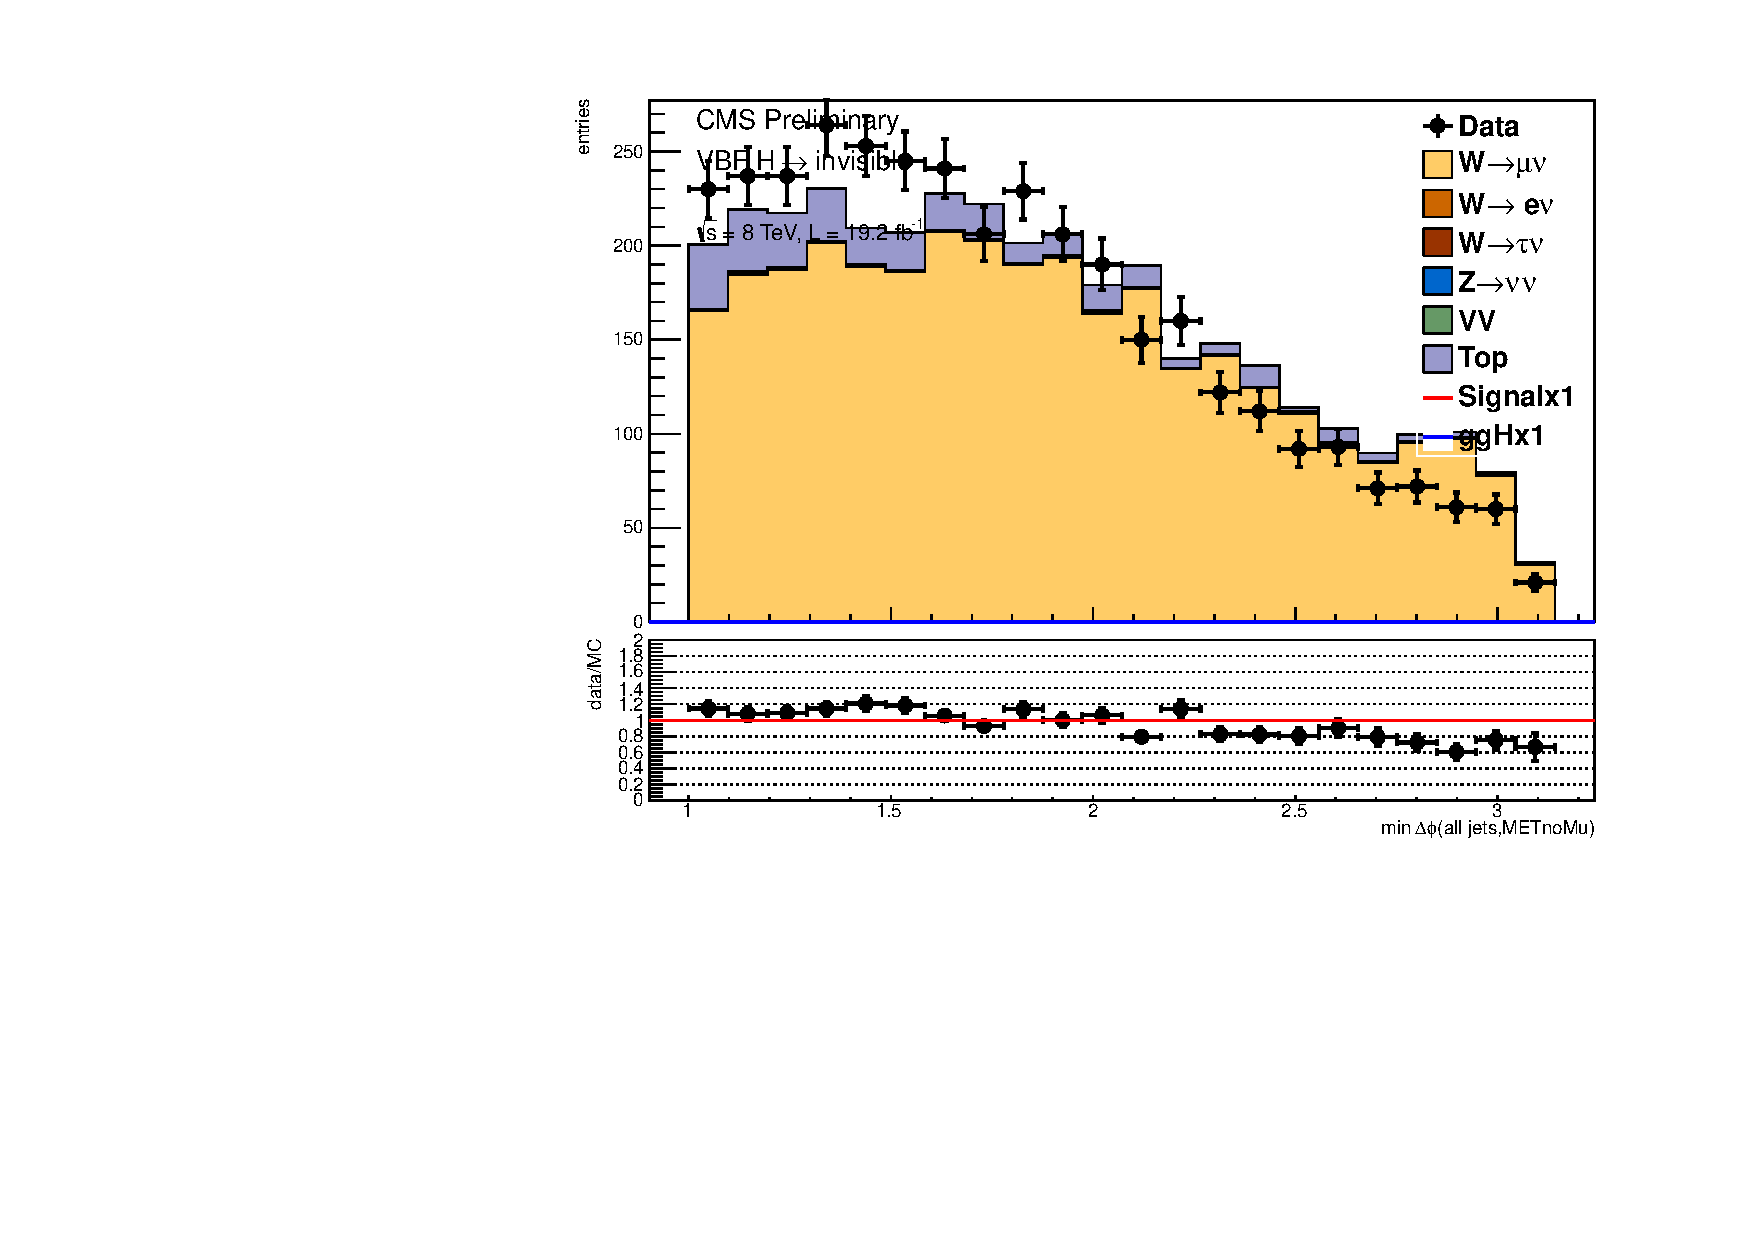
\includegraphics[clip=true,trim=0 0 0 20,width=.95\textwidth]{TalkPics/hig14038preapproval/output_presel/munu_alljetsmetnomu_mindphi.pdf}

    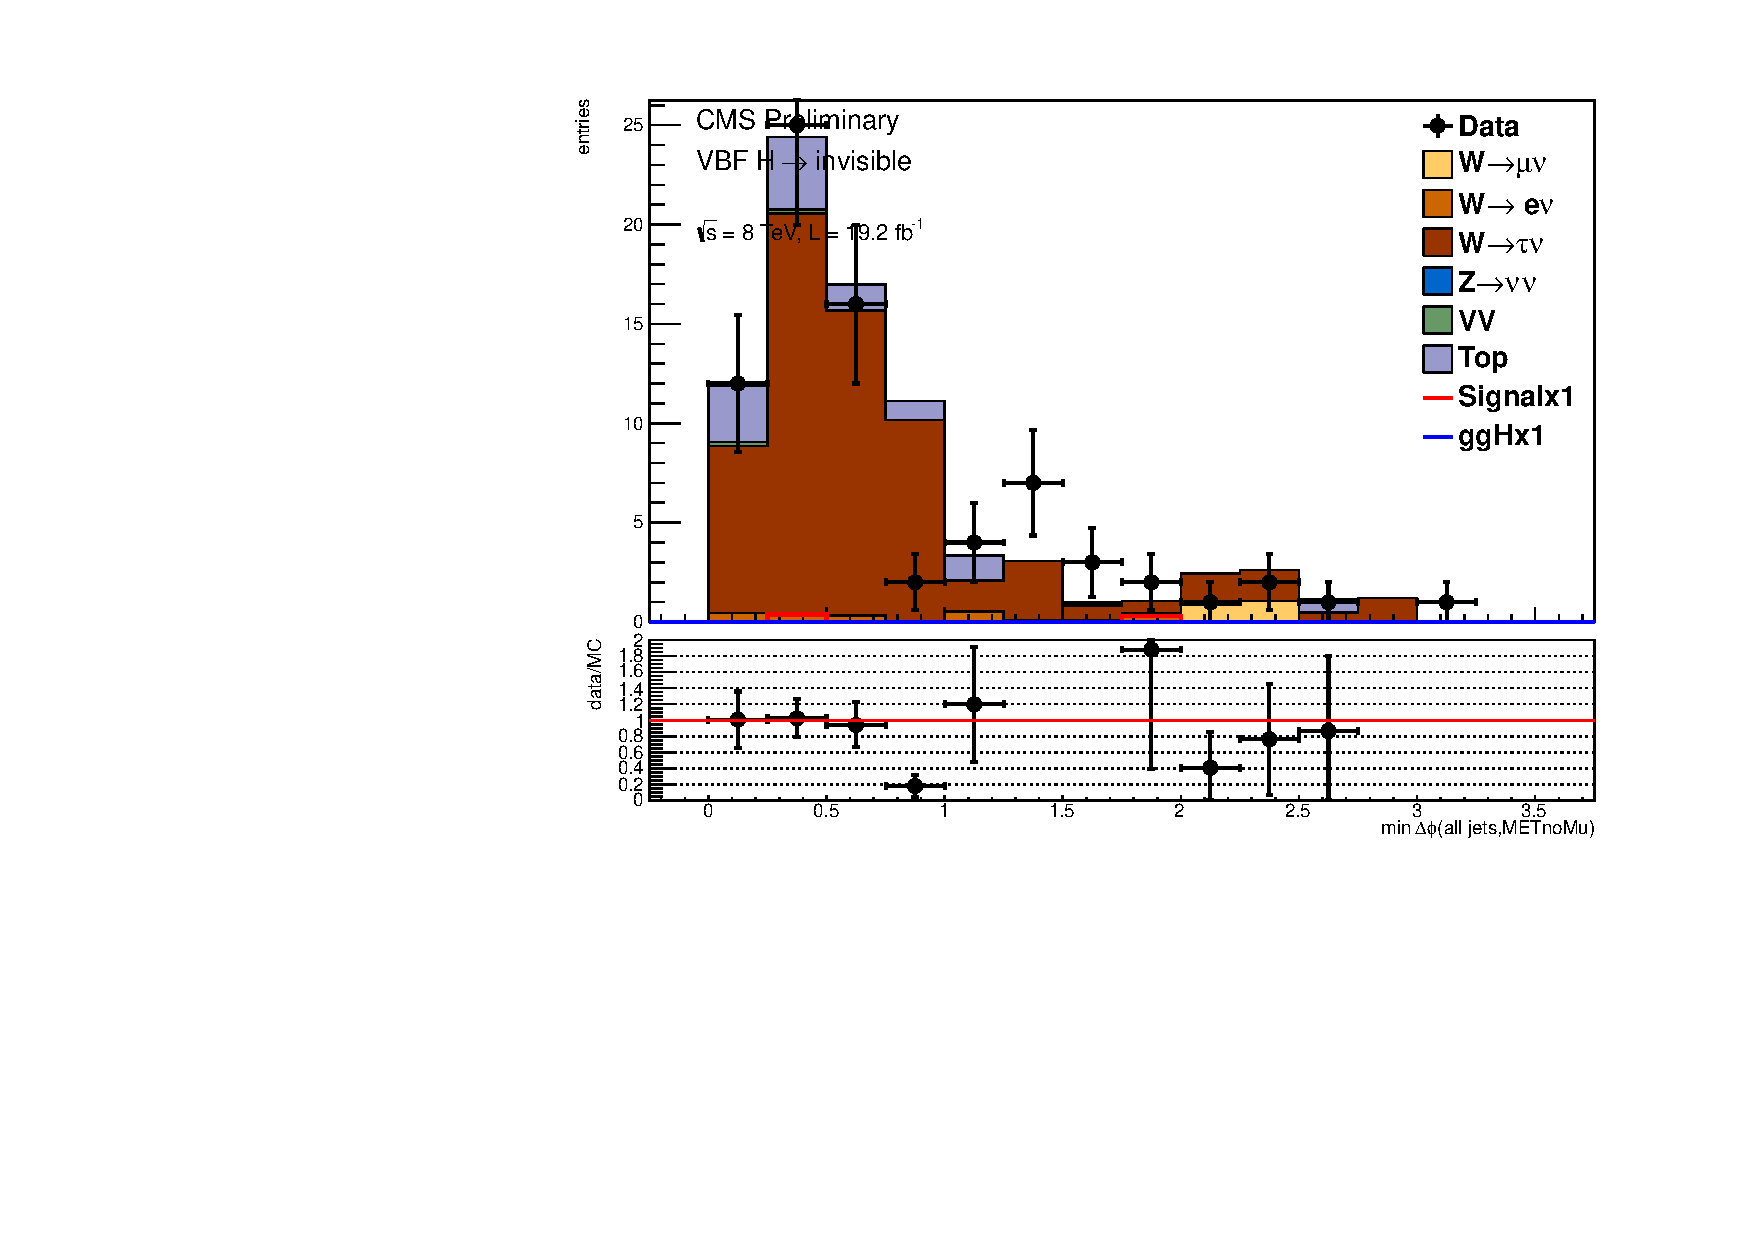
\includegraphics[clip=true,trim=0 0 0 20,width=.95\textwidth]{TalkPics/hig14038preapproval/output_sigreg/taunu_alljetsmetnomu_mindphi.pdf}
  \end{columns}
  \end{columns}
\end{frame}


\begin{frame}
  \frametitle{$Z\rightarrow \nu\nu$}
  \vspace{-.35cm}
  \begin{columns}
    \column{1.1\textwidth}
  \begin{block}{}
    \vspace{-.1cm}
    \scriptsize
    \begin{itemize}
    \item Data-MC agreement good for limited statistics
    \item Same method used as for prompt analysis
    \end{itemize}
    \vspace{-.2cm}
    \centering
\begin{tabular}{|l|c|c|}
\hline
 & Signal region & Control region \\
 \hline
$N^{data}$ & XXX & $18 \pm 4.2 (stat.)$\\
$N^{bkg}$ & N/A  & $0.2 \pm 0.1 (stat.)$  \\
$N^{MC}(EWK)$ & $7.9 \pm 0.2 (stat.)$  & $6.0 \pm 0.2 (stat.) $   \\
$N^{MC}(QCD)$ & $29.5 \pm 3.0 (stat.)$  & $20.7 \pm 2.5 (stat.) $   \\
 \hline
 $\frac{N^{data}-N^{bkg}}{N^{MC}(EWK)+N^{MC}(QCD)}$ & \multicolumn{2}{|c|}{$0.67\pm 0.16 (stat.) \pm 0.06 (MC stat.)$} \\
 \hline
$Final N^{Z\rightarrow\nu\nu} estimate$ & \textcolor{red}{$157.3 \pm 37.6 (data stat.) \pm 18.2 (MC stat.)$}  & N/A  \\
\hline
\end{tabular}
    
  \end{block}
  \end{columns}
  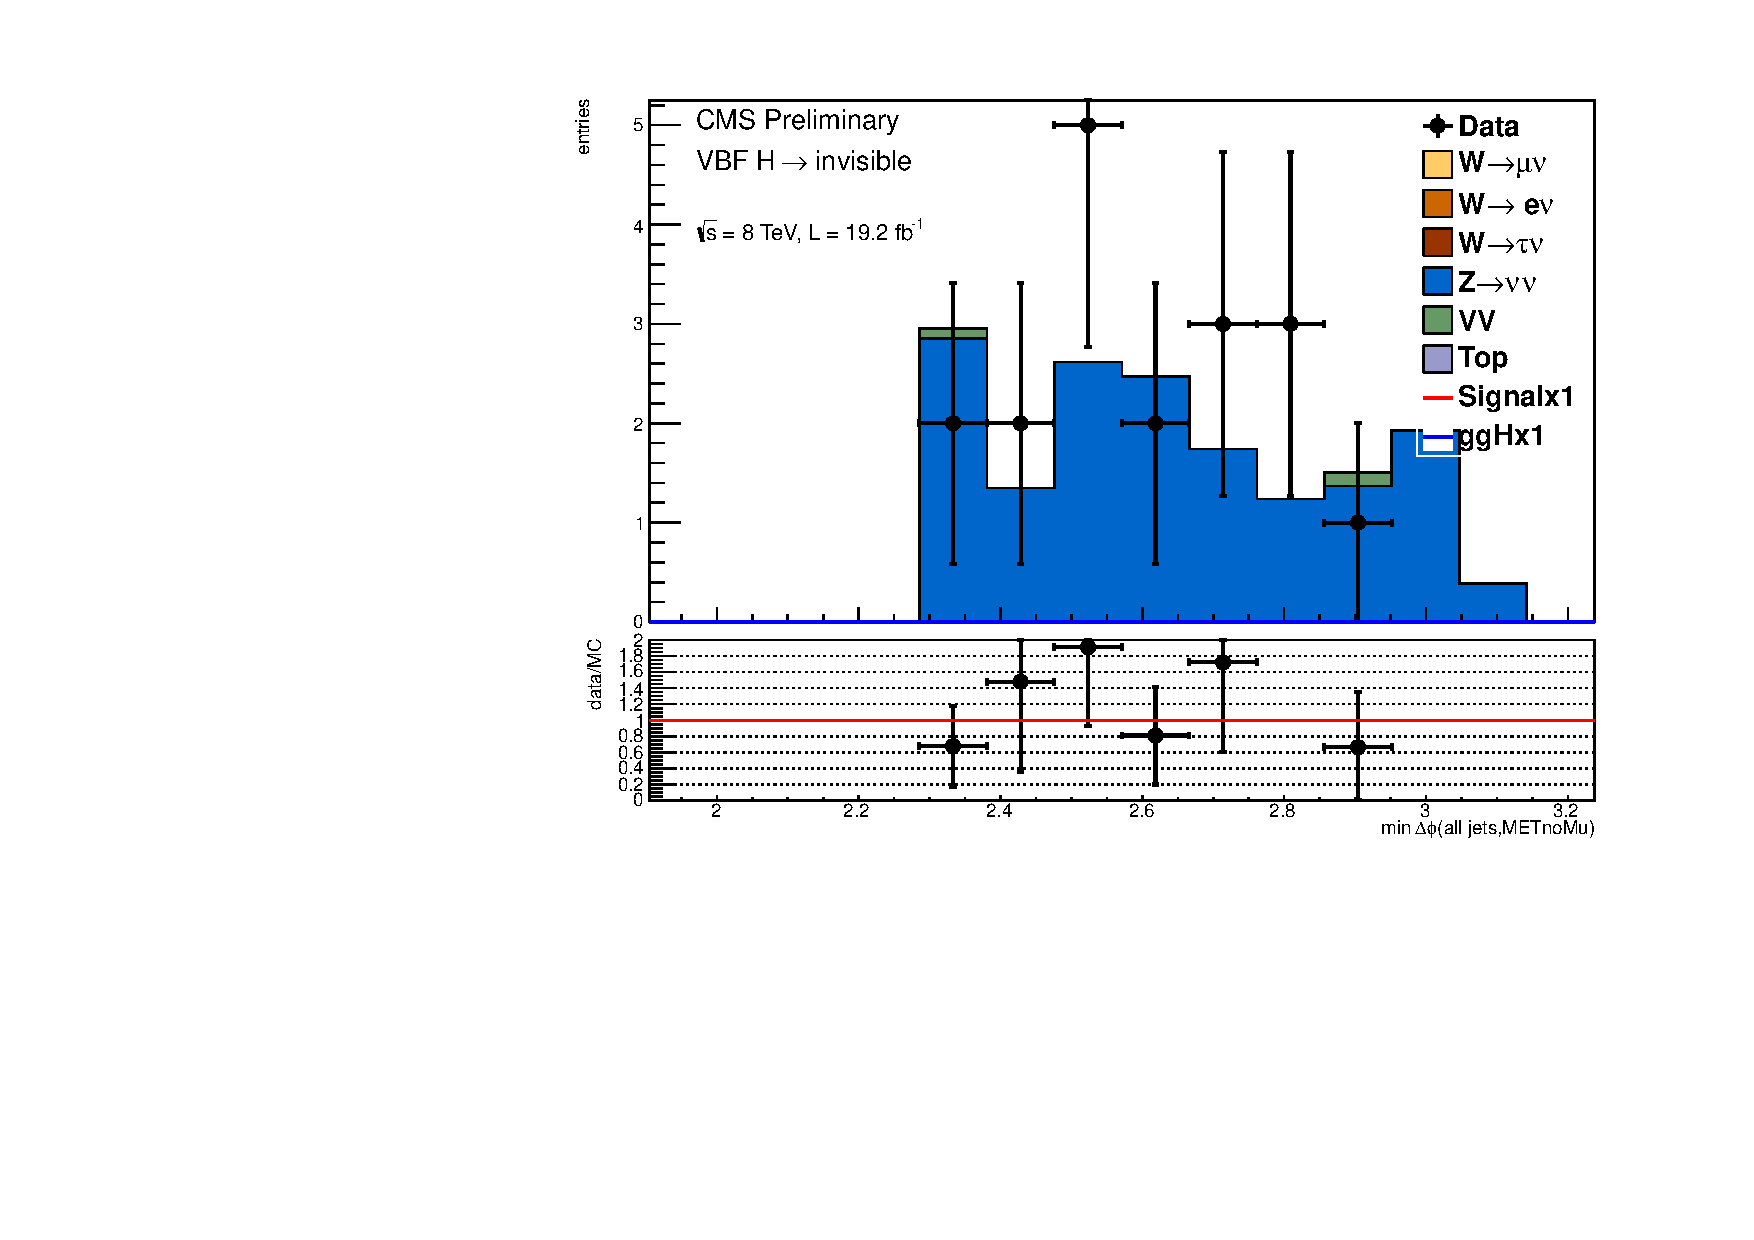
\includegraphics[clip=true,trim=0 0 0 20,width=.5\textwidth,height=.4\textheight]{TalkPics/hig14038preapproval/output_sigreg/mumu_alljetsmetnomu_mindphi}
  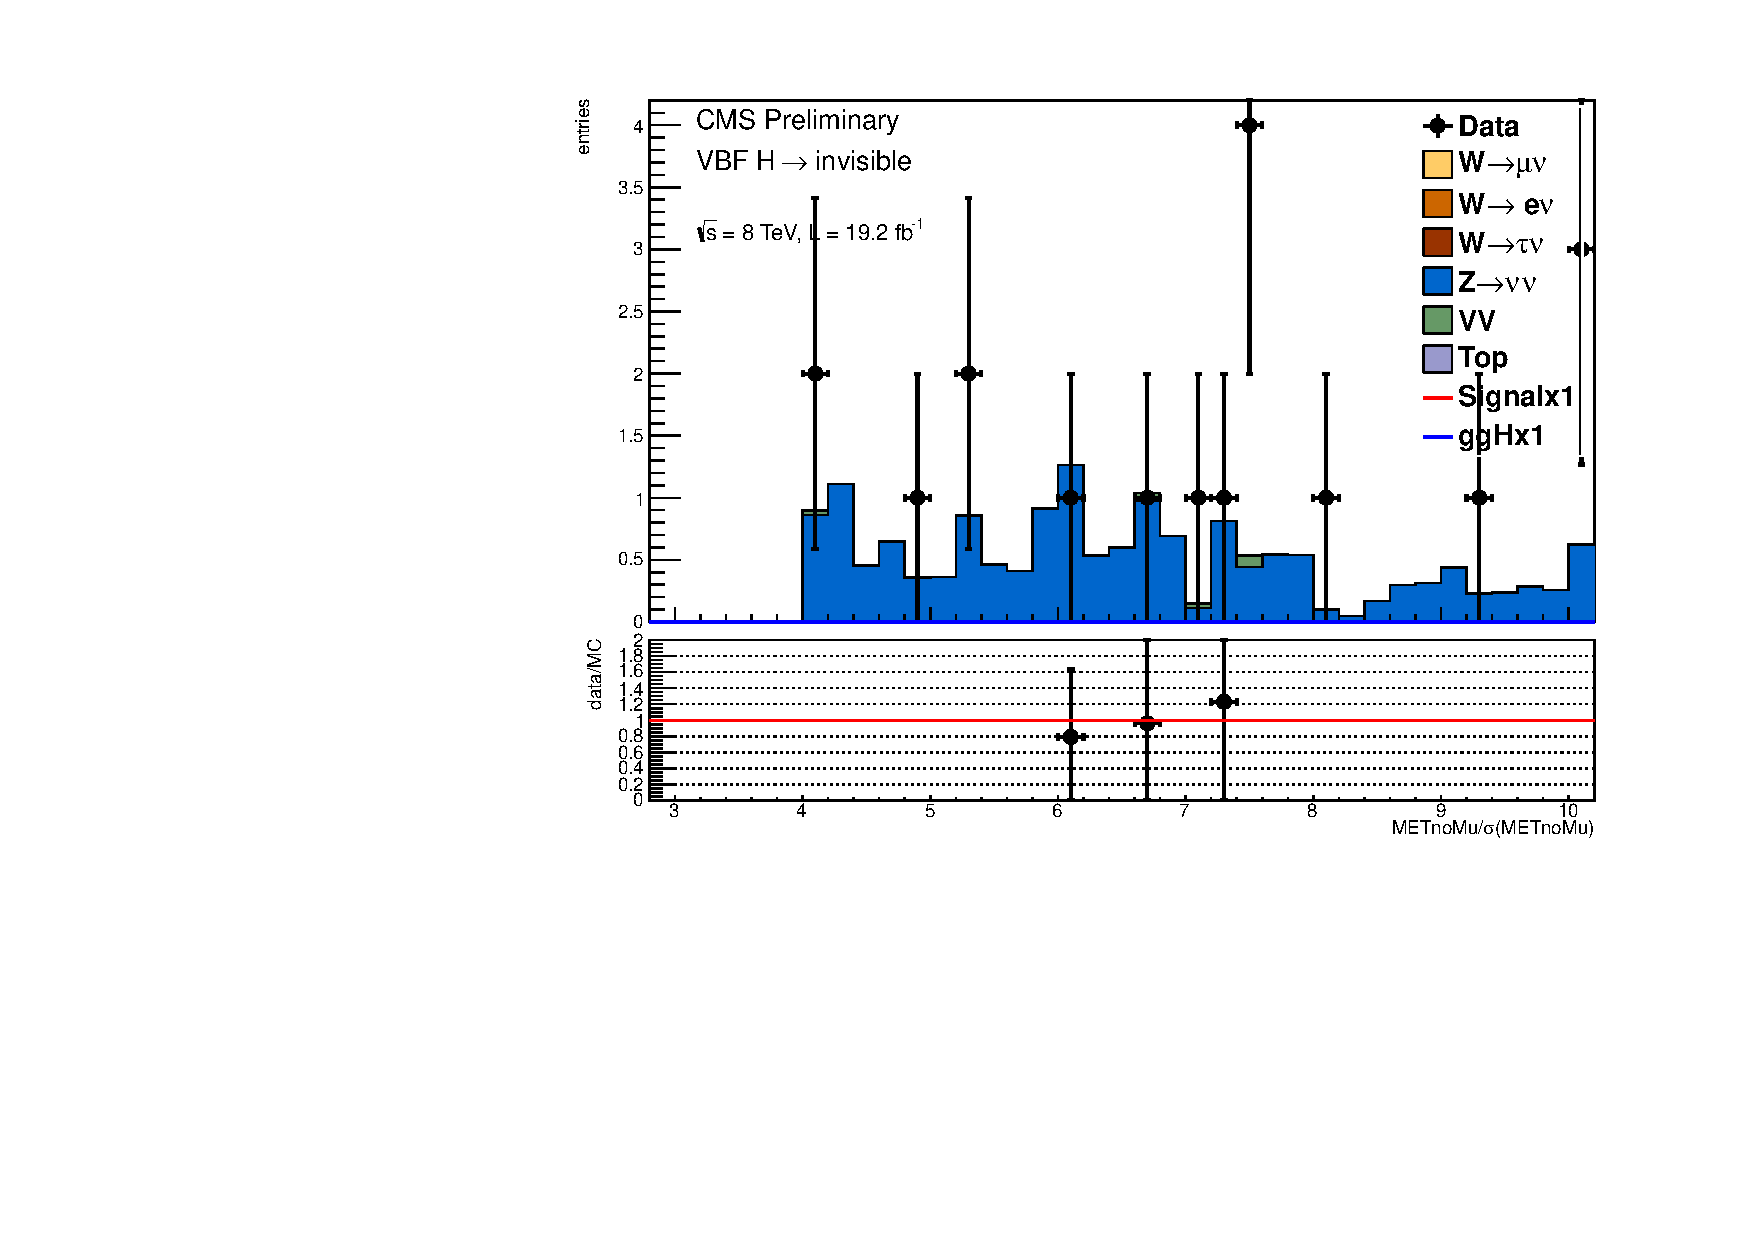
\includegraphics[clip=true,trim=0 0 0 20,width=.5\textwidth,height=.4\textheight]{TalkPics/hig14038preapproval/output_sigreg/mumu_metnomu_significance}
\end{frame}

\begin{frame}
  \frametitle{Normalisation variation}
  \vspace{-.2cm}
  \scriptsize Jet met dphi

  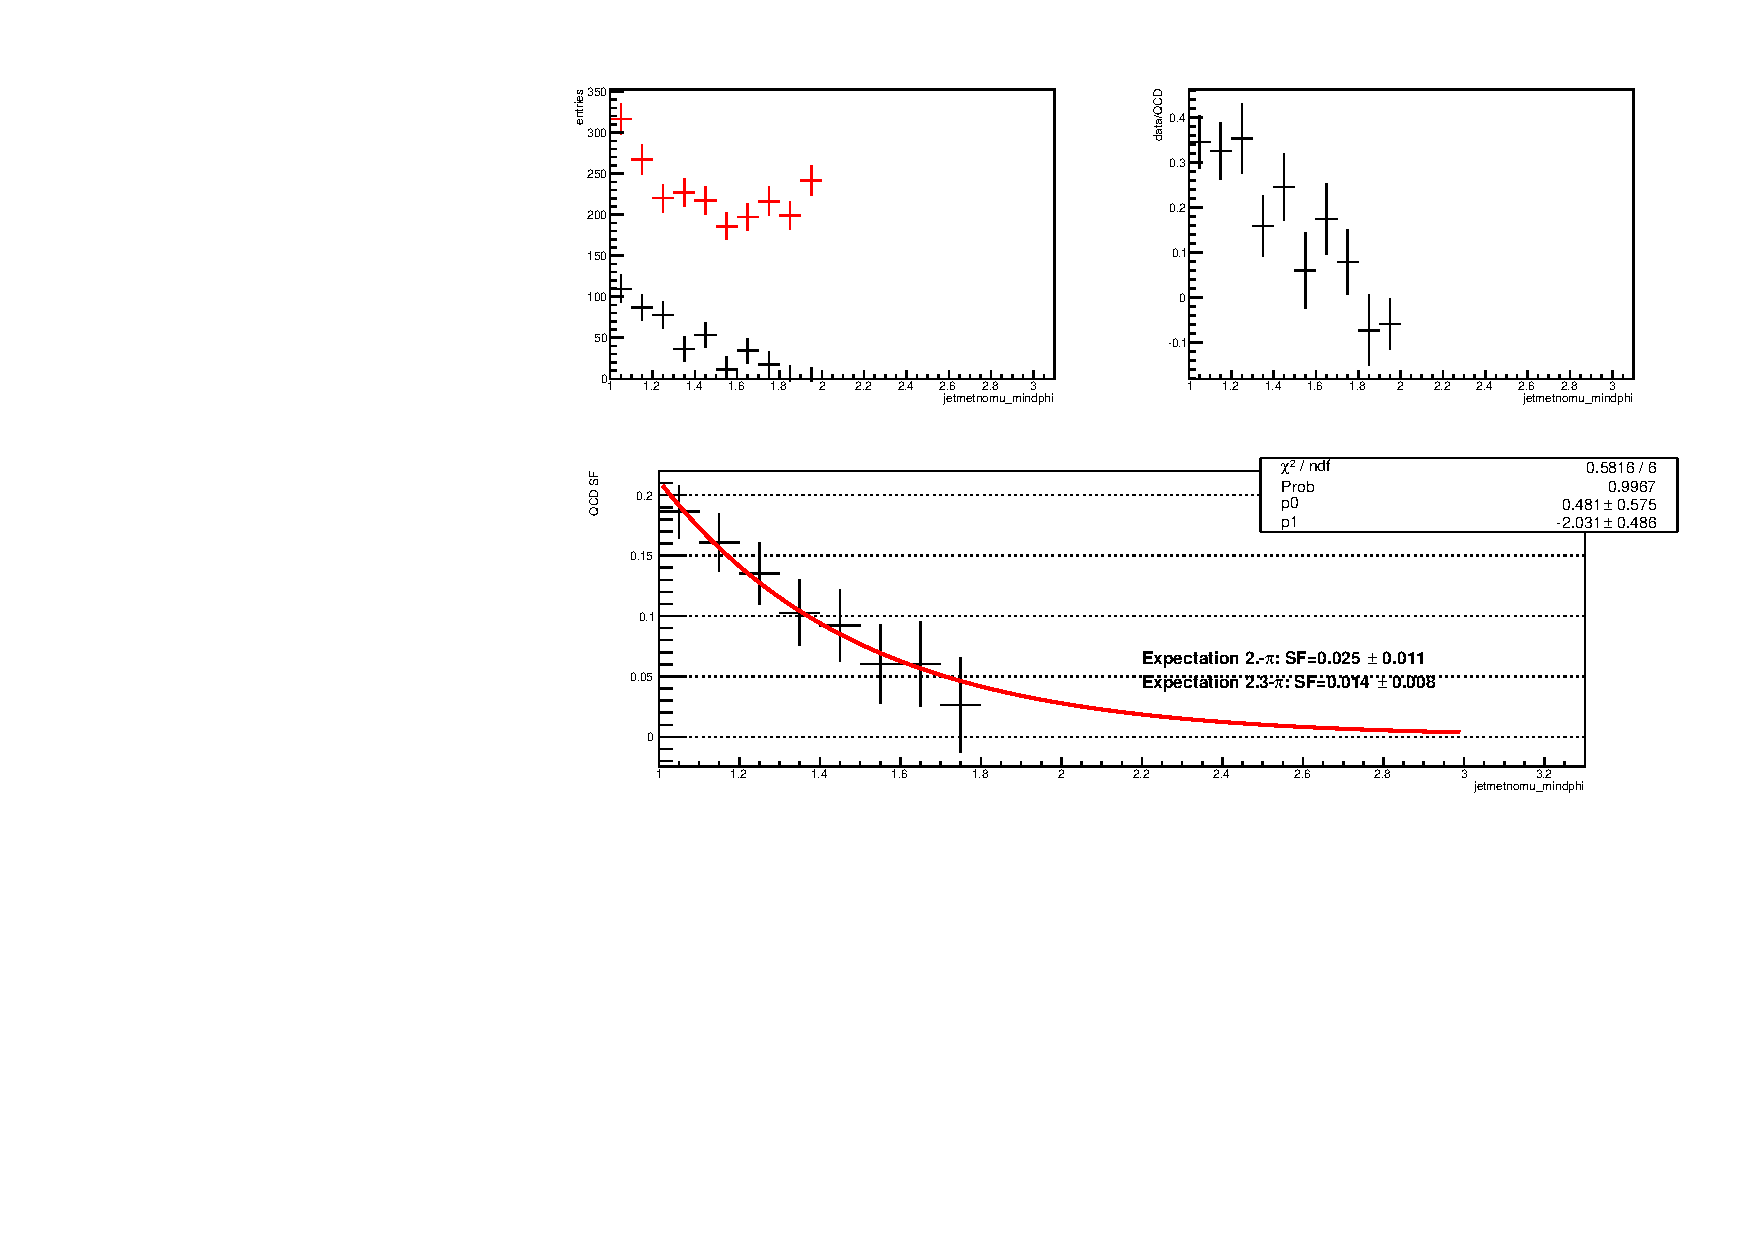
\includegraphics[clip=true,trim=0 0 0 180,width=.9\textwidth]{TalkPics/hig14038preapproval/qcdEstimate/jetmetnomu_mindphi_norm1_SF.pdf}

  \vspace{-.2cm}

  \scriptsize MET significance


  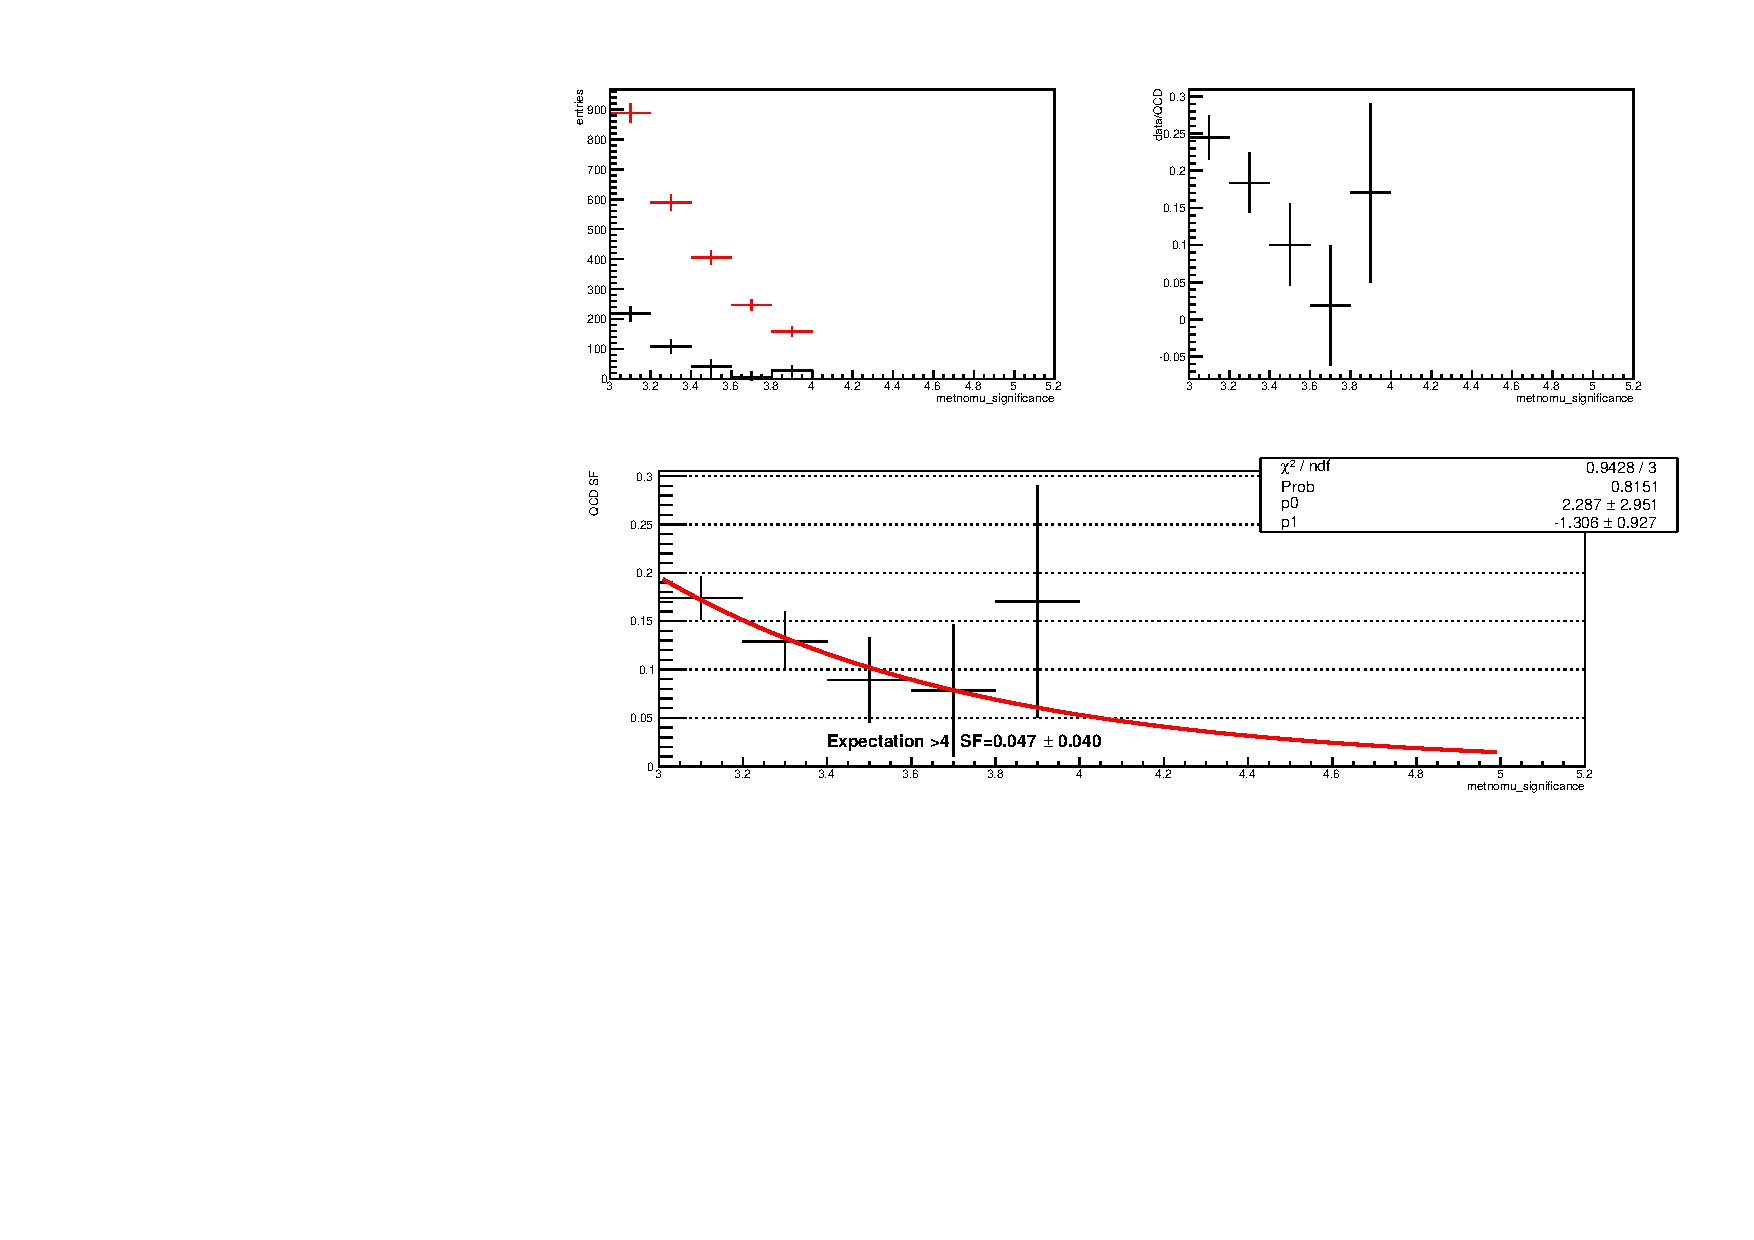
\includegraphics[clip=true,trim=0 0 0 190,width=.9\textwidth]{TalkPics/hig14038preapproval/qcdEstimate/metnomu_significance_norm1_SF.pdf}
\end{frame}

\begin{frame}
  \frametitle{QCD background estimation: Result and systematics}
  \begin{columns}
    \column{.75\textwidth}
     \begin{block}{}
       \centering
       \scriptsize
       \begin{tabular}{|l|c|c|c|}
         \hline
         Region & Factor & Extrapolation & Extrapolation \\
         & & mindphi$>2.5$ & metsig$>4$ \\
         \hline
         \rowcolor{yellow} Norm 1 & 0.17 $\pm$ 0.02 & 0.014 $\pm$ 0.008 & 0.05 $\pm$ 0.04\\
         Norm 1+2 & 0.12 $\pm$ 0.01 & 0.013 $\pm$ 0.004 & 0.01 $\pm$ 0.01 \\
         Norm 1+3 & 0.24 $\pm$ 0.03 & 0.03 $\pm$ 0.01 & 0.55 $\pm$ 0.06 \\
         Norm 2 & 0.06 $\pm$ 0.01 & - & 0.01 $\pm$ 0.02 \\
         Norm 3 & 0.5 $\pm$ 0.1 & 0.21 $\pm$ 0.11 & - \\
         \hline
       \end{tabular}
     \end{block}
     \end{columns}
     \begin{block}{}
       \scriptsize
       \begin{itemize}
       \item Good agreement in mindphi extrapolations
       \item Norm 3 agreement in metsig is poor
       \item[-] As norm 3 has low statistics and is an odd region: drop
       \item Use envelope of norm 1 scale factors
       \item Final prediction: $N_{S}^{QCD}=17\pm 14$ 
       \end{itemize}
     \end{block}
\end{frame}

\begin{frame}
  \frametitle{Systematics}
  \begin{block}{}
  \scriptsize
  \begin{itemize}
  \item Changes are:
  \item[-] Top background now data driven so has data stat. error
  \item[-] New $W\rightarrow\tau\nu$ extrapolation error
  \item[-] QCD background error procedure now as described above
  \item We are reevaluating the $Z/\gamma^{*}\rightarrow\mu\mu$ to $Z\rightarrow\nu\nu$ with aMC@NLO
  \item[-] Waiting on MC jobs, very quick to update results
  \end{itemize}
  \end{block}
\end{frame}

%SYSTEMATICS
\begin{frame}
  \frametitle{Systematics}
  \begin{block}{}
    \scriptsize
    \begin{itemize}
    \item Uncertainties considered are mostly the same as the prompt analysis
    \item[-] Details in backup
    \item The size of each uncertainty is given as a percentage of total signal/background
    \item[-] Still statistically dominated
    \end{itemize}
  \centering
  \vspace{-.2cm}
  \begin{tabular}{lcc}
    \hline
    Source  & Total background & Signal     \\
    \hline
    Control region data stat. & 9.30 & 0.00 \\
    $Z/\gamma^{*}\rightarrow\mu\mu$ to $Z\rightarrow\nu\nu$ extrapolation & 7.16 & 0.00 \\
    MC stat. & 5.54 & 3.82 \\
    Jet energy scale & 4.94 & 10.70 \\
    $W\rightarrow\tau\nu$ control region extrapolation & 4.46 & 0.00 \\
    Lepton ID efficiency & 3.22 & 0.00 \\
    QCD normalisation & 3.18 & 0.00 \\
    Jet energy resolution & 2.86 & 1.81 \\
    Unclustered energy scale & 2.28 & 1.64 \\
    Pileup weight & 0.95 & 1.56 \\
    Luminosity & 0.02 & 2.60 \\
    Theory Uncertainty & 0.01 & 5.14\\
    \hline
  \end{tabular}
\end{block}
\end{frame}



%SOURCE OF GAIN
\begin{frame}
  \frametitle{Source of gain}
  \vspace{-.3cm}
  \begin{columns}
    \column{1.05\textwidth}
  \begin{block}{}
    \scriptsize
    \begin{itemize}
    \item Expected limits from prompt and parked analyses have been obtained from the prompt and parked data
    \item ggH signal and UES uncertainty not included
    \item[-] This explains 2\% difference in parked cuts parked trigger number
    \item Data driven top control region used for both prompt and parked cuts
    \item Prompt trigger weights ignore correlations in turn on part of parked cut region
    \end{itemize}
    \scriptsize
    \vspace{-.15cm}
    \centering
    \begin{tabular}{|l|c|c|}
      \hline
      & Prompt trigger & parked trigger \\
      \hline
      Prompt cuts & 45\% & 46\% \\
      Parked cuts & 47\% & 40\% \\
      \hline
    \end{tabular}
  \end{block}
  \vspace{-.3cm}
  \begin{block}{\scriptsize Interpretation}
    \scriptsize
    \begin{itemize}
    \item Prompt cuts limits $\sim$ same as old card with both prompt and parked trigger
    \item[-] slight difference as paper limit had extra $W\gamma$
    \item The parked cuts give a worse limit with prompt trigger than with parked trigger
    \item Improvement comes from using the new phase space made available by the parked trigger
    \end{itemize}
  \end{block}
  \end{columns}
\end{frame}

\begin{frame}
  \frametitle{Uncertainty impact table - impacts larger than 0\%}
  \vspace{-.3cm}
  \begin{columns}
    \column{1.05\textwidth}
  \begin{block}{}
    \scriptsize    
    \centering
        \begin{tabular}{|l|c|c|}
\hline
Expected limit with: & All Nuisances: 37.8\% & No Nuisances: 14.3\% \\
\hline
\hline
Nuisance      &                Removal effect (relative \%) &  Addition effect (relative \%) \\
\hline
$Z\rightarrow\nu\nu$ data stat.:     &-12.4\%                &         65.8\% \\
$Z\rightarrow\nu\nu$ extrapolation:  & -8.3\%                &         53.5\% \\
JES:                                 & -6.5\%                &         12.2\% \\
$W\rightarrow\tau\nu$ extrapolation: & -4.1\%                &         24.5\% \\
$Z\rightarrow\nu\nu$ MC stat.:       & -2.6\%                &         24.5\% \\
$W\rightarrow\tau\nu$ MC stat.:      & -1.5\%                &         12.2\% \\
$W\rightarrow\tau\nu$ data stat.:    & -1.5\%                &         13.6\% \\
QCD normalisation:                   & -1.5\%                &          7.5\% \\
$W\rightarrow\mu\nu$ MC stat.:       & -1.0\%                &          6.1\% \\
Muon ID efficiency:                  & -0.5\%                &          6.8\% \\
Tau ID efficiency:                   & -0.5\%                &          5.5\% \\
$W\rightarrow e\nu$ data stat.:      & -0.5\%                &          4.8\% \\
$W\rightarrow\mu\nu$ data stat.:     & -0.5\%                &          3.4\% \\
$W\rightarrow e\nu$ MC stat.:        & -0.5\%                &          3.4\% \\
Electron ID efficiency:              &  0.0\%                &          0.6\% \\
PU weight:                           &  0.0\%                &          0.6\% \\
\hline
    \end{tabular}
  \end{block}
  \end{columns}
\end{frame}

%DATA AND MC SAMPLES LIST
\begin{frame}
  \frametitle{Data Samples}
  \begin{columns}
    \column{1.1\textwidth}
  \begin{block}{}
    \centering
    \scriptsize
     \begin{tabular}{| l | c |}
    \hline
    Dataset/JSON & Int. Lumi [pb$^{-1}$] \\
    \hline
    /MET/Run2012A-22Jan2013-v1/AOD & 889 \\
    /VBF1Parked/Run2012B-22Jan2013-v1/AOD & 3871 \\
    /VBF1Parked/Run2012C-22Jan2013-v1/AOD & 7152 \\
    /VBF1Parked/Run2012D-22Jan2013-v1/AOD & 7317 \\


    \hline
    Total analysed & 19229 \\
    \hline
    Cert\_190456-208686\_8TeV\_22Jan2013ReReco\_Collisions12\_JSON.txt & 19789 \\
    \hline
  \end{tabular}
     \end{block}
  \end{columns}
\end{frame}

\begin{frame}
  \frametitle{MC Samples-1}
  \begin{columns}
\column{1.15\textwidth}
  \begin{block}{}
    \scriptsize
    \centering
    \begin{tabular}{| l | c | c | c |}
  \hline
  Dataset & $\sigma$ [pb] & No. of Events & Eq. $\int L$ [fb$^{-1}$] \\
  \hline
  ($Z \rightarrow \nu\nu$) + jets (50 $<$ HT $<$ 100 GeV) & 381.2 & 4040980 & 10.6 \\
  ($Z \rightarrow \nu\nu$) + jets (100 $<$ HT $<$ 200 GeV) & 160.3 & 4416646 & 27.6 \\
  ($Z \rightarrow \nu\nu$) + jets (200 $<$ HT $<$ 400 GeV) & 41.49 & 5055885 & 122 \\
  ($Z \rightarrow \nu\nu$) + jets (400 $<$ HT $<$ $\infty$ GeV) & 5.274 & 1006928 & 191 \\
  ($W \rightarrow l\nu$) + jets (inclusive) & 37509(NNLO) & 76102995 & 2.03 \\
  ($W \rightarrow l\nu$) + 1 jet & 5400 & 23141598 & 42.9 \\
  ($W \rightarrow l\nu$) + 2 jet & 1750 & 34044921 & 19.5 \\
  ($W \rightarrow l\nu$) + 3 jet & 519 & 15539503 & 29.9 \\
  ($W \rightarrow l\nu$) + 4 jet & 214 & 13382803 & 62.5 \\
  ($Z/\gamma ∗ \rightarrow ll$) + jets (Mll $>$ 50) & 3503.71(NNLO) & 30459503 & 8.7 \\
  ($Z/\gamma ∗ \rightarrow ll$) + 1 jets (Mll $>$ 50) & 561 & 24045248 & 42.9 \\
  ($Z/\gamma ∗ \rightarrow ll$) + 2 jets (Mll $>$ 50) & 181 & 21852156 & 121 \\
  ($Z/\gamma ∗ \rightarrow ll$) + 3 jets (Mll $>$ 50) & 51.1 & 11015445 & 216 \\
  ($Z/\gamma ∗ \rightarrow ll$) + 4 jets (Mll $>$ 50) & 23.04 & 6402827 & 278 \\
  EWK ($Z/\gamma ∗ \rightarrow ll$) + 2 jets & 0.888 & 2978717 & 3354 \\
  EWK ($W^{+} \rightarrow l\nu$) + 2 jets & 6.48 & 8996164 & 1388 \\
  EWK ($W^{-} \rightarrow l\nu$) + 2 jets & 4.09 & 5994018 & 1466 \\
  \hline
  \end{tabular}
    \end{block}
  \end{columns}
  \end{frame}

\begin{frame}
  \frametitle{MC Samples-2}
  \begin{block}{}
    \scriptsize
    \centering
    \begin{tabular}{| l | c | c | c |}
  \hline
  Dataset & $\sigma$ [pb] & No. of Events & Eq. $\int L$ [fb$^{-1}$] \\
  \hline
  WW & 54.838(NLO) & 10000431 & 182 \\
  WZ & 33.21(NLO) & 10000283 & 301 \\
  ZZ & 17.654(NLO) & 9799908 & 555 \\
  $W \gamma$ & 461.6 & 4802358 & 10.4 \\
  tt + jets & 245.8(NNLO) & 6923750 & 28.2 \\
  t (t-channel) & 56.4(NLO) & 3758227 & 66.6 \\
  t (tW-channel) & 11.1(NLO) & 497658 & 44.8 \\
  t (s-channel) & 3.79(NLO) & 259961 & 68.6 \\
  $\bar{t}$ (t-channel) & 30.7(NLO & 1935072 & 63.0 \\
  $\bar{t}$ (tW-channel) & 11.1(NLO) & 493460 & 44.5 \\
  $\bar{t}$ (s-channel) & 1.76(NLO) & 139974 & 79.5 \\
  \hline
\end{tabular}
  \end{block}
\end{frame}

%ADD OBJECTS INFO
\begin{frame}
  \frametitle{Objects}
  \begin{columns}
    \column{.5\textwidth}
    \vspace{-.3cm}
    \begin{block}{\scriptsize PFMET}
      \scriptsize
      \begin{itemize}
      \item Ignore muons
      \item Type0+1 corrections
      \item Smeared PFMET for MC
      \end{itemize}
    \end{block}
    \vspace{-.3cm}
    \begin{block}{\scriptsize AK5 PFJets}
      \scriptsize
      \begin{itemize}
      \item L1FastJet+L2+L3(+L2L3Residual) JEC
      \item ``Loose'' PF Jet ID
      \item Cleaned with veto leptons
      \item ``Loose'' PU jet ID
      \item Smeared jet collection for MC (JER is smeared to match data)
      \end{itemize}
    \end{block}
    \column{.5\textwidth}
    \vspace{-.3cm}
    \begin{block}{\scriptsize Veto leptons}
      \scriptsize
      \begin{itemize}
      \item loose+PFiso muons $p_{T}>10$ GeV, $|\eta|<2.1$
      \item veto+PFiso electrons $p_{T}>10$ GeV, $|\eta|<2.4$
      \end{itemize}
    \end{block}
    \vspace{-.3cm}
    \begin{block}{\scriptsize Tight leptons}
      \scriptsize
      \begin{itemize}
      \item As veto leptons but ``tight'' ID and $p_{T}>20$ GeV
      \end{itemize}
    \end{block}
    \vspace{-.3cm}
    \begin{block}{\scriptsize Hadronic taus}
      \scriptsize
      \begin{itemize}
      \item $p_{T}>20$ GeV, $|\eta|<2.3$,$d_{Z}<0.2$ cm
      \item Tight ID, discriminant ``byTightCombinedIsolationDeltaBetaCorr3Hits''
      \item Efficiency $\sim$0.55, fake rate 0.02(barrel),0.03(endcap)

      \end{itemize}
    \end{block}
  \end{columns}
\end{frame}

\begin{frame}
  \frametitle{Data/MC reweighting}
  \begin{block}{}
    \begin{itemize}
    \item We apply the following reweightings of the MC to match the data:
    \item[-] Trigger efficiency
    \item[-] Lepton efficiency: ID and isolation
    \item[-] Pileup distribution
    \end{itemize}
  \end{block}
\end{frame}


\begin{frame}
  \frametitle{Other approaches investigated and run 2 prospects}
  \begin{block}{\scriptsize Initial investigations}
    \scriptsize
    \begin{itemize}{}
    \item Planned to define a loose pre-selection and model QCD shape
    \item Several options for analysis strategy:
    \item[-] Rectangular cuts and counting experiment
    \item[-] Rectangular cuts and shape experiment
    \item[-] MVA and counting experiment
    \item[-] MVA and shape experiment
    \item Due to trigger conditions no appropriate QCD control region found - details later
    \end{itemize}
  \end{block}

    \begin{block}{\scriptsize Run 2 prospects}
    \scriptsize
    \begin{itemize}
    \item Prescaled looser control triggers planned to enable better QCD control region
    \item Will reinvistigate shape analysis and MVA
    \end{itemize}
    \end{block}
\end{frame}

%FRAMEWORK STRATEGY AND SYNC
\begin{frame}
  \frametitle{Software framework strategy}
  \begin{block}{\scriptsize Prompt analysis}
    \scriptsize
    \begin{itemize}
    \item Two frameworks: Analyses A and B
    \item independent ntuples and analysis code
    \end{itemize}
  \end{block}
  \begin{block}{\scriptsize Parked analysis}
      \scriptsize
      \begin{itemize}
      \item Insufficient manpower to maintain and develop two frameworks
      \item Moved to one fully developed framework
      \item[-] New framework is development of analysis B and uses same ntuples
      \item Synchronised yields in signal and control regions between new framework and old analyses A and B
      \item Repeated expected limit calculation from HIG-13-030 analysis with the new framework and parked data
      \item[-] Agrees with HIG-13-030 to within 2\%, which is good given rereco, and change of global tag and triggers
      \end{itemize}
  \end{block}
\end{frame}

\begin{frame}
  \frametitle{Software cross check}
  \begin{block}{}
    \begin{itemize}
    \item Starting point region numbers also cross-checked in alternate software
    \item[-] Agreement is better than 0.5\%
    \end{itemize}
  \end{block}
\end{frame}

\begin{frame}
  \frametitle{Signal efficiency as a function of PU}
  \begin{block}{}
    \centering
    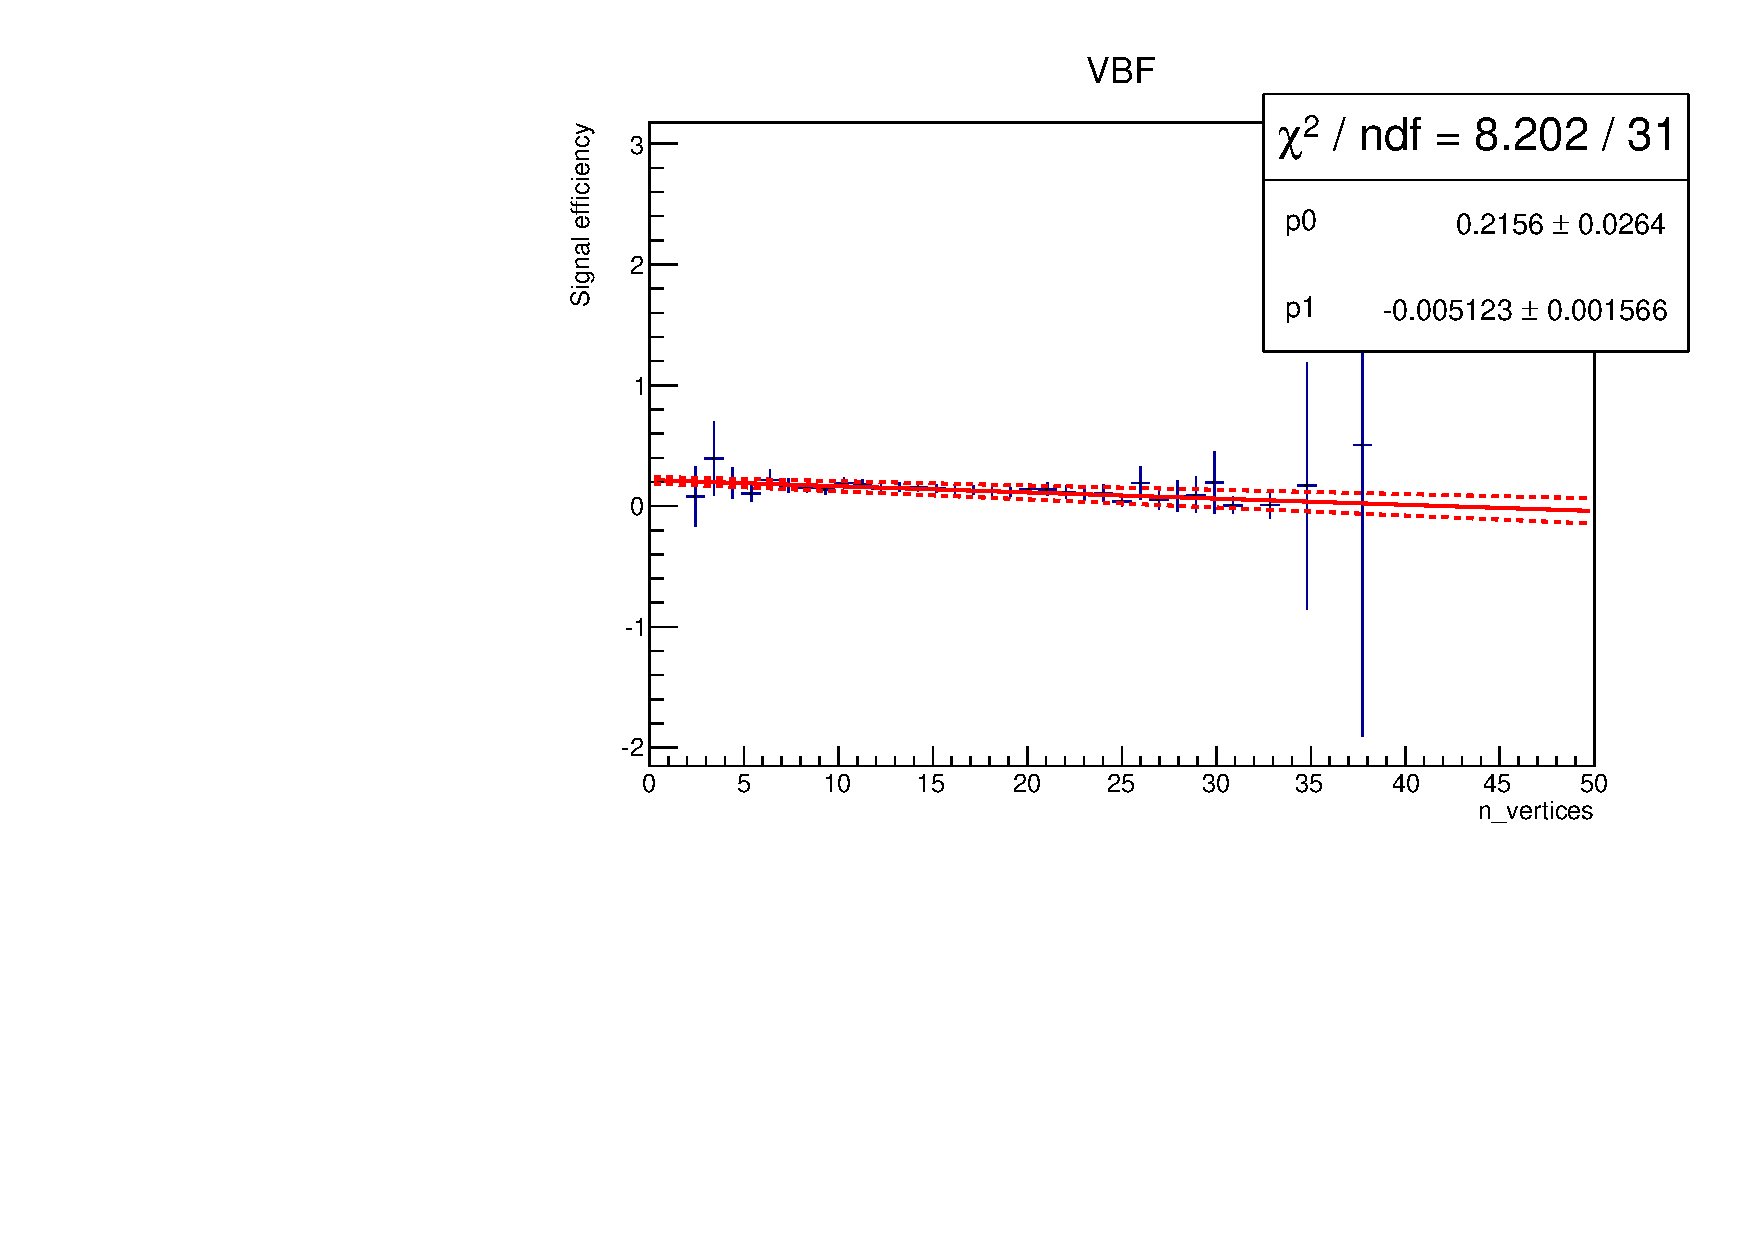
\includegraphics[width=.8\textwidth]{TalkPics/invupdate081214/vbfsigeff.pdf}
  \end{block}
\end{frame}

\begin{frame}
  \frametitle{Signal efficiency as a function of PU}
  \begin{block}{}
    \centering
    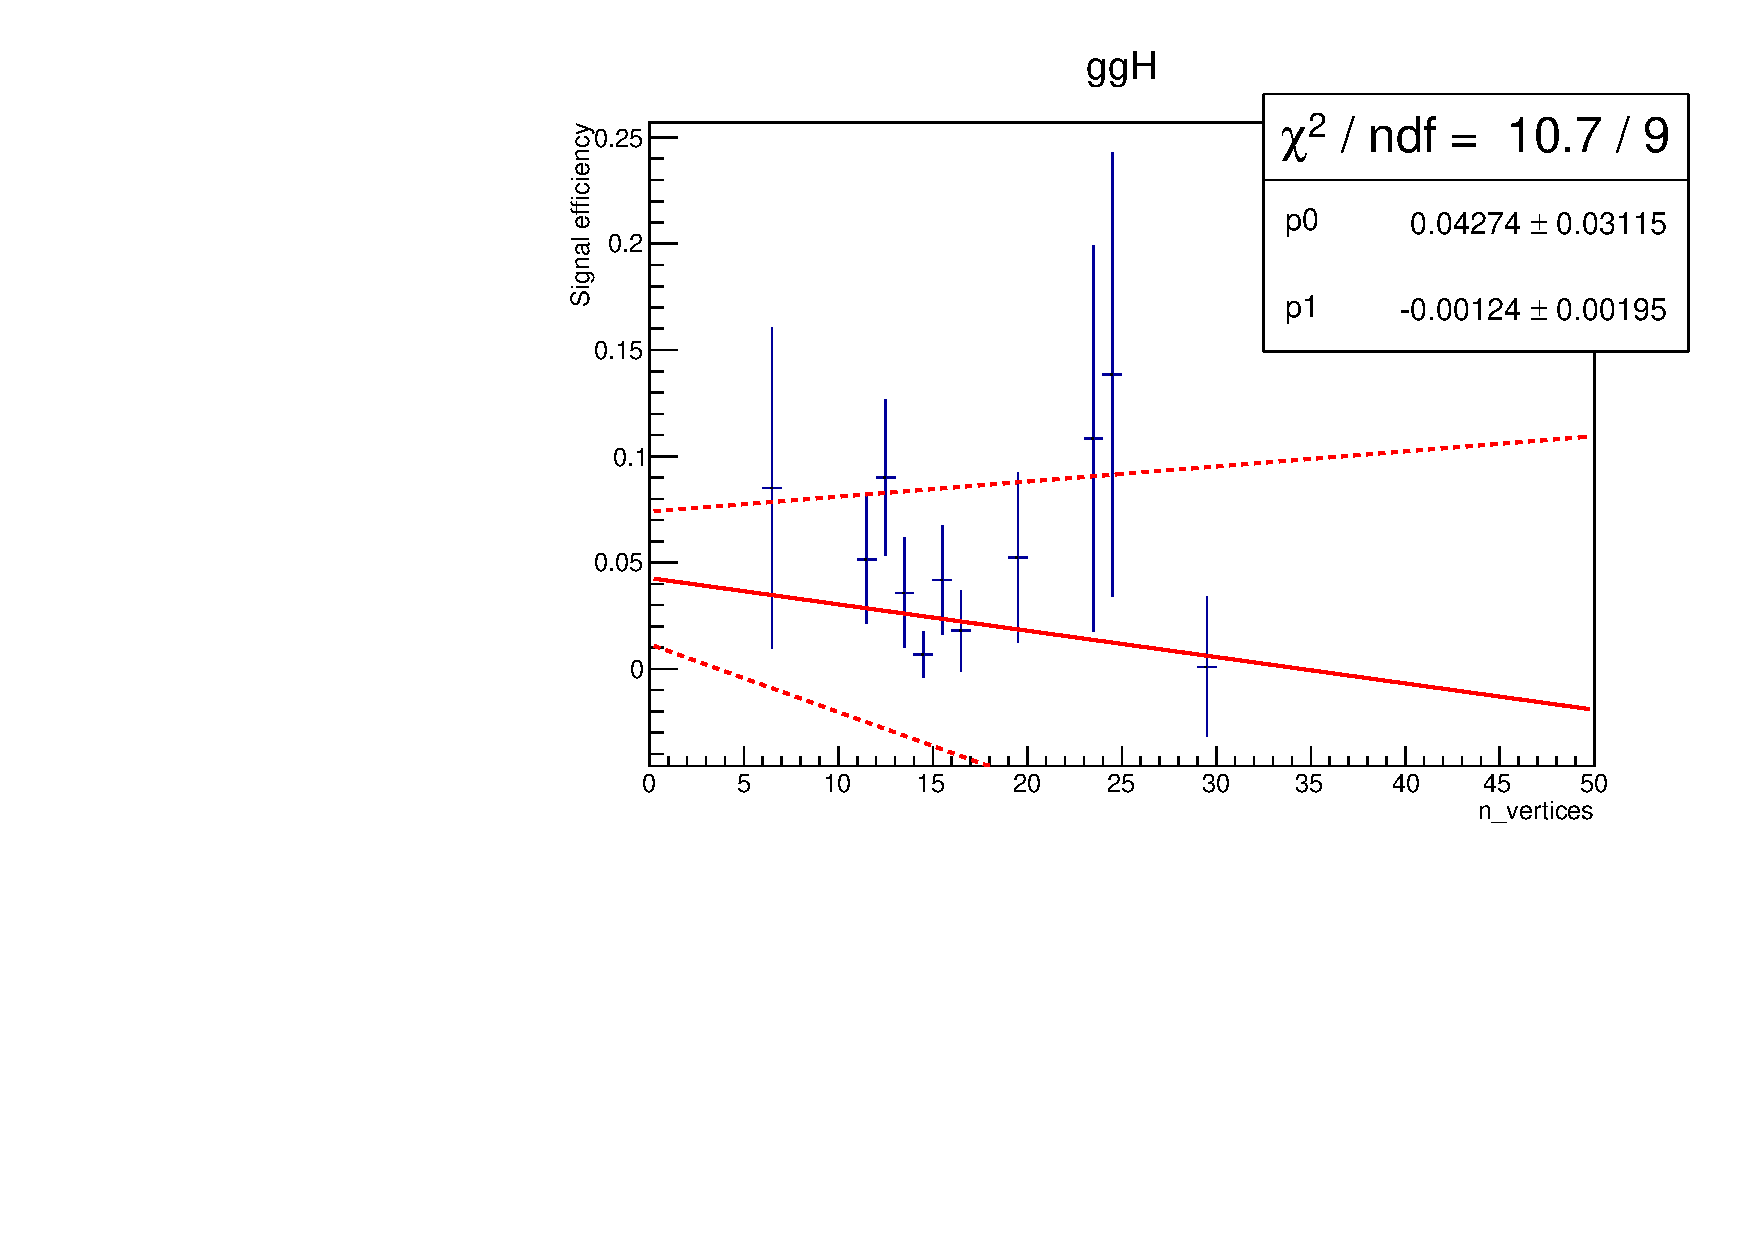
\includegraphics[width=.8\textwidth]{TalkPics/invupdate081214/gghsigeff.pdf}
  \end{block}
\end{frame}

\begin{frame}
  \frametitle{Veto muons in signal MC}
  \begin{block}{}
    \scriptsize
    \begin{itemize}
    \item Veto muons don't have a dz or dxy cut
    \item Concern that we would be vetoing muons from a different vertex
    \item Muon veto efficiency turns out to be very high:
    \item[-] $\sim$10 signal MC events with a veto muon out of $\sim$55000
    \item nvetomuons doesn't seem correlated with PU
    \end{itemize}
    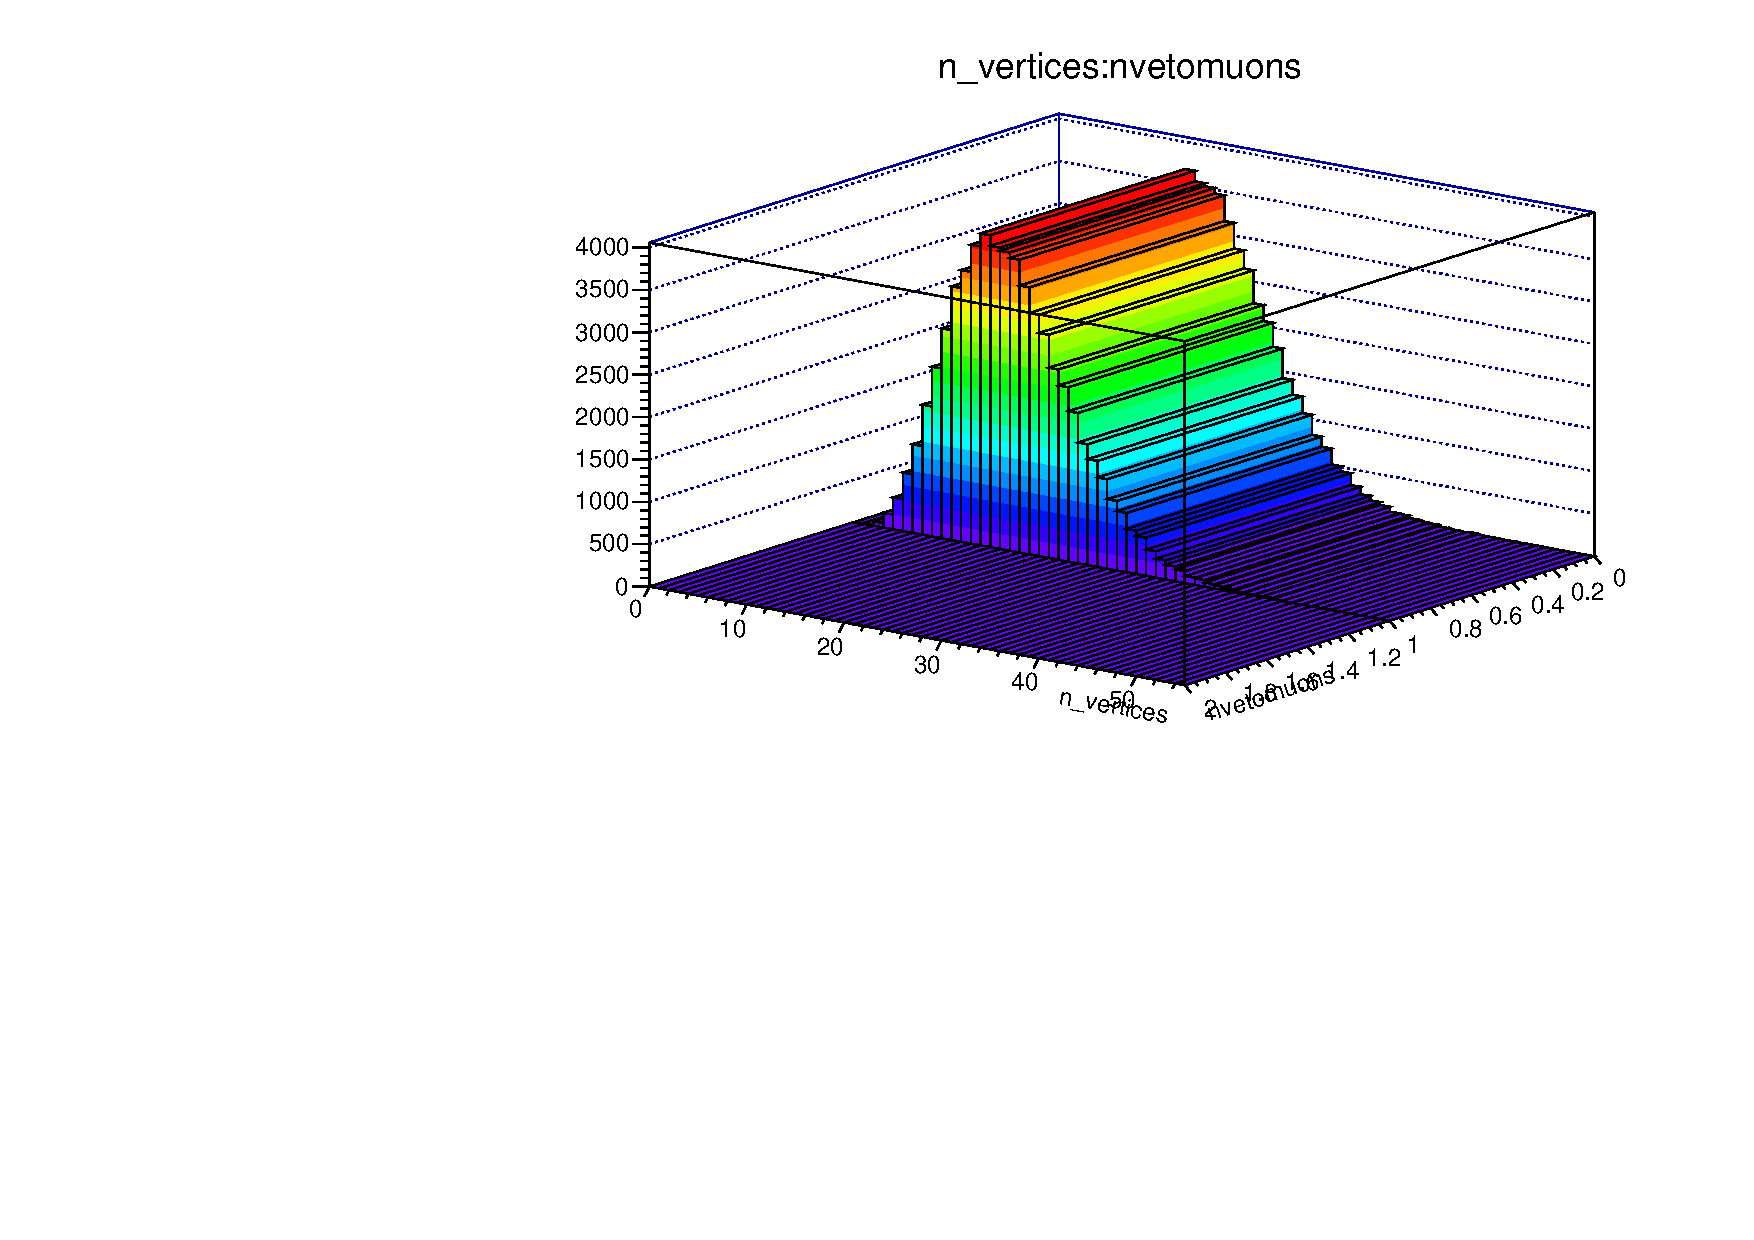
\includegraphics[width=.5\textwidth]{TalkPics/invupdate081214/vetomuvsPU.pdf}
    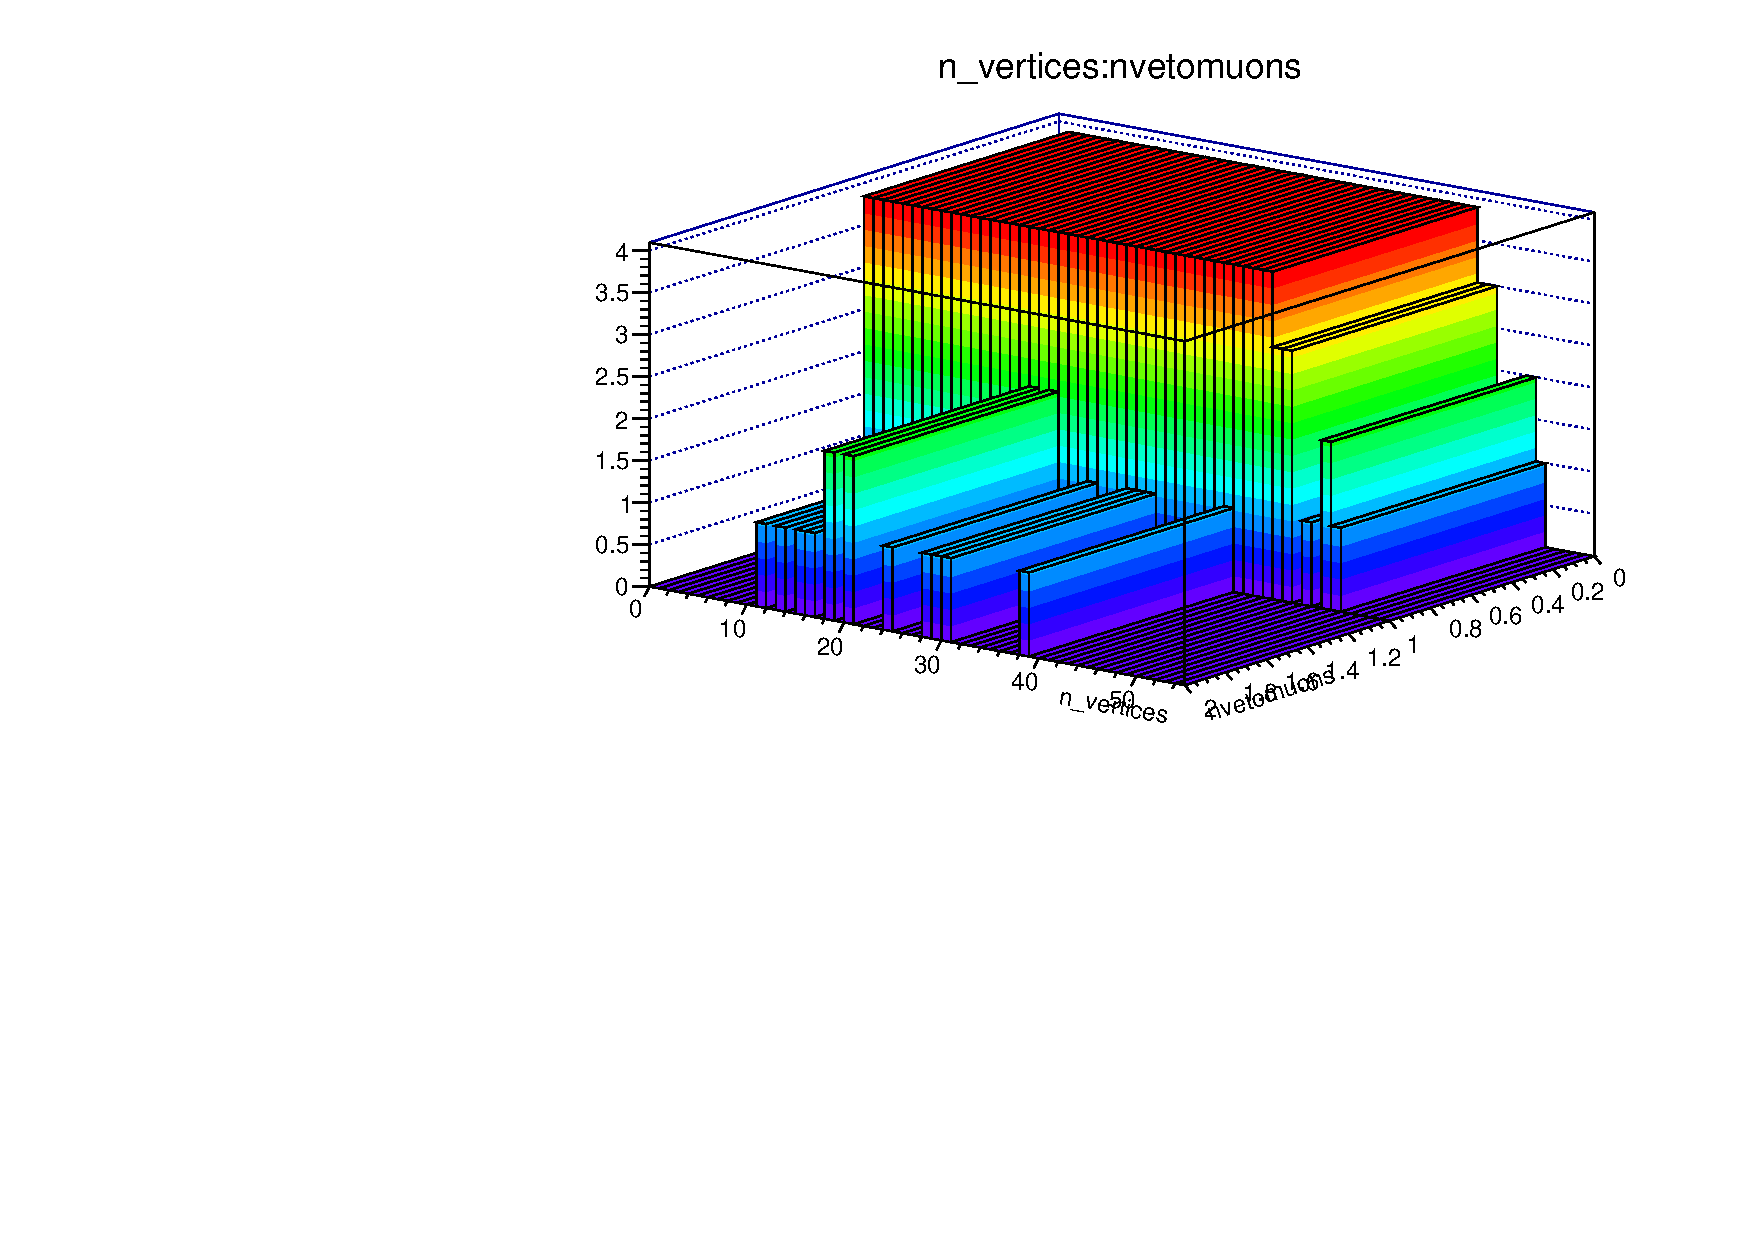
\includegraphics[width=.5\textwidth]{TalkPics/invupdate081214/vetomuvsPUzoom.pdf}
    \scriptsize
    \begin{itemize}
    \item Right plot is zoom of left
    \end{itemize}
  \end{block}
\end{frame}

%LIMIT AS A FUNCTION OF Z EXTRAP UNC
\begin{frame}
  \frametitle{Effect of $Z/\gamma^{*}\rightarrow\mu\mu$ to $Z\rightarrow\nu\nu$ uncertainty}
  \begin{block}{}
    \scriptsize
    \centering
    \begin{tabular}{|l|c|}
      \hline
      Uncertainty/\% & Median expected limit/\% \\
      \hline
      20 & 37.79 \\
      10 & 35.64 \\
      9 & 35.45 \\
      5 & 34.86 \\
      0 & 34.67 \\
      \hline
    \end{tabular}
    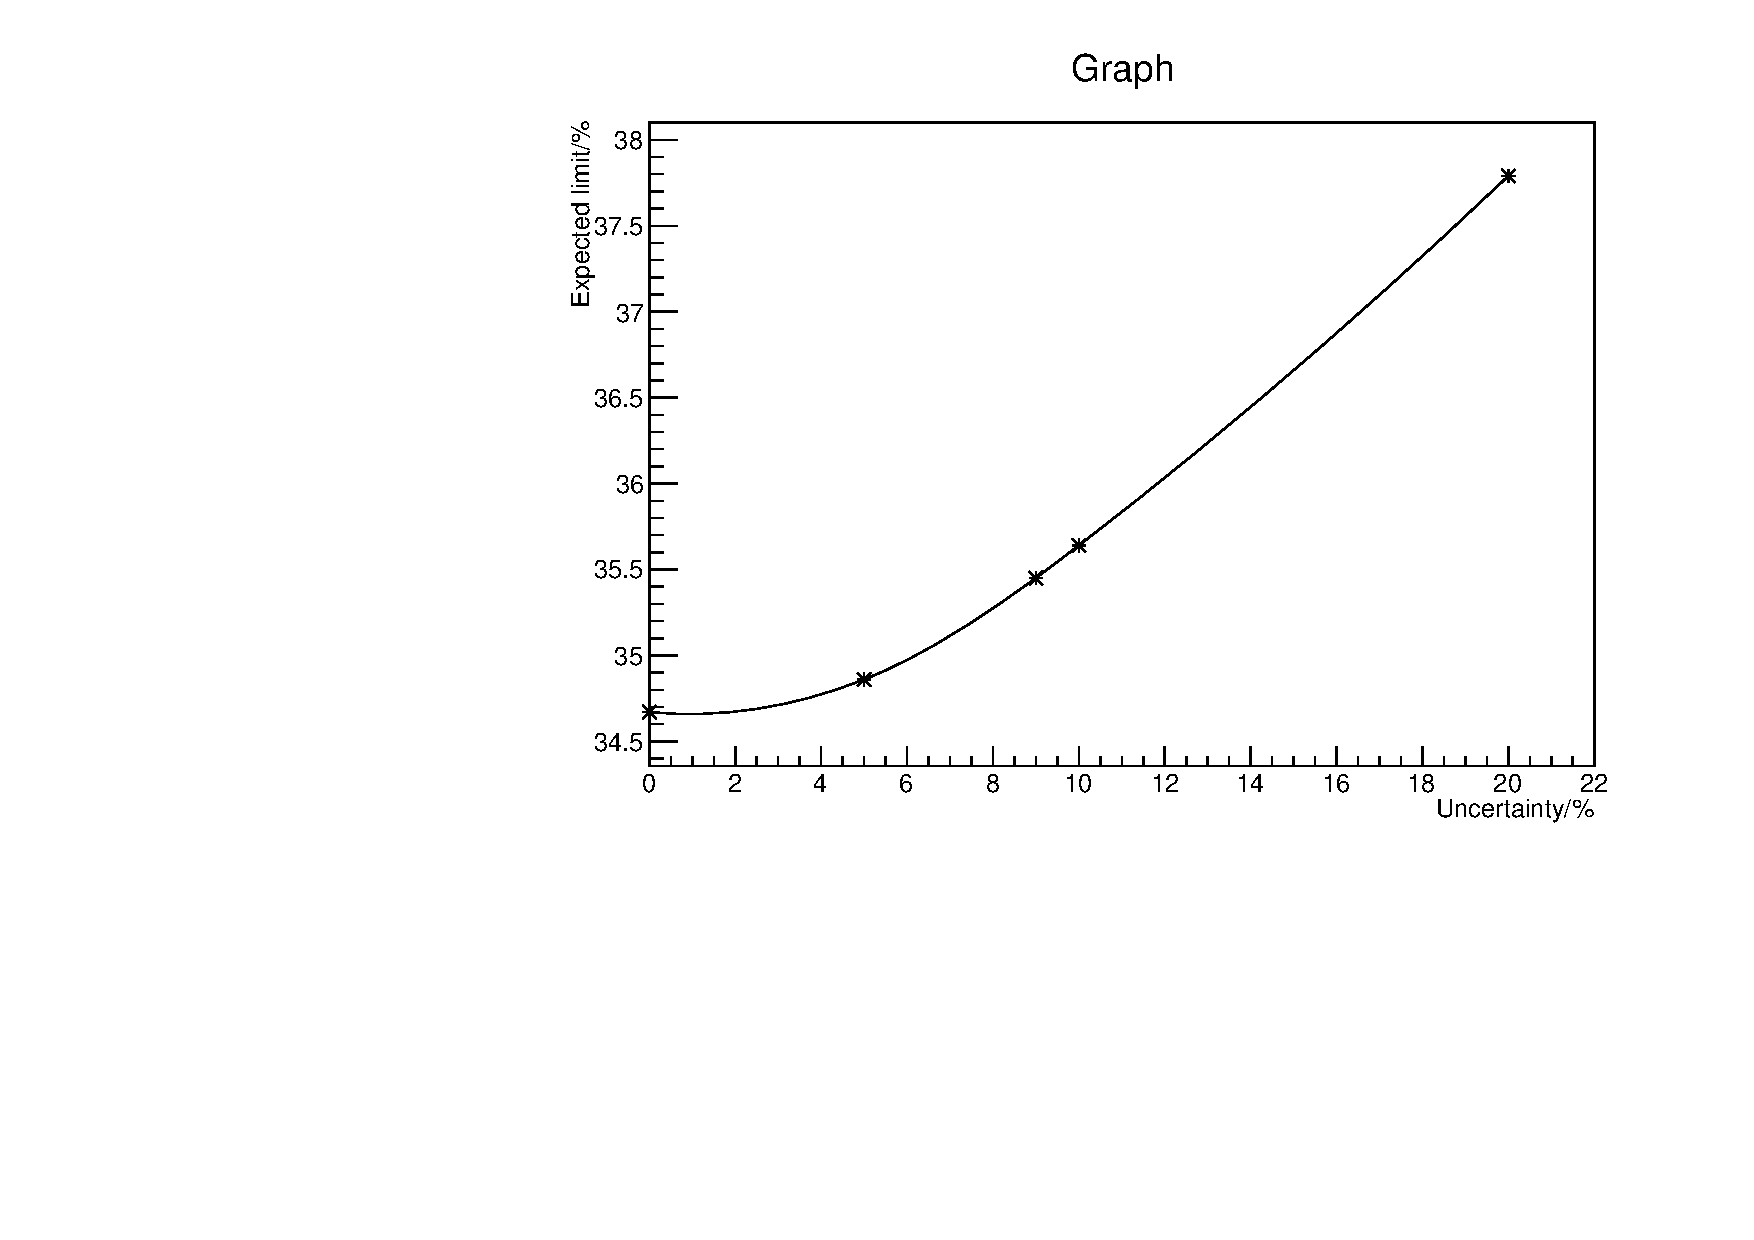
\includegraphics[width=.5\textwidth]{TalkPics/hig14038preapproval/zvvextrapgraph.pdf}
  \end{block}
\end{frame}

%CONTROL PLOTS
\begin{frame}
  \frametitle{Signal Region Control Plots}
  \vspace{-.2cm}
  \begin{block}{}
    \vspace{-.1cm}
  \begin{columns}
    \column{.45\textwidth}
    \scriptsize
    $\text{Min}\Delta\phi(\text{MET,all jets})$
  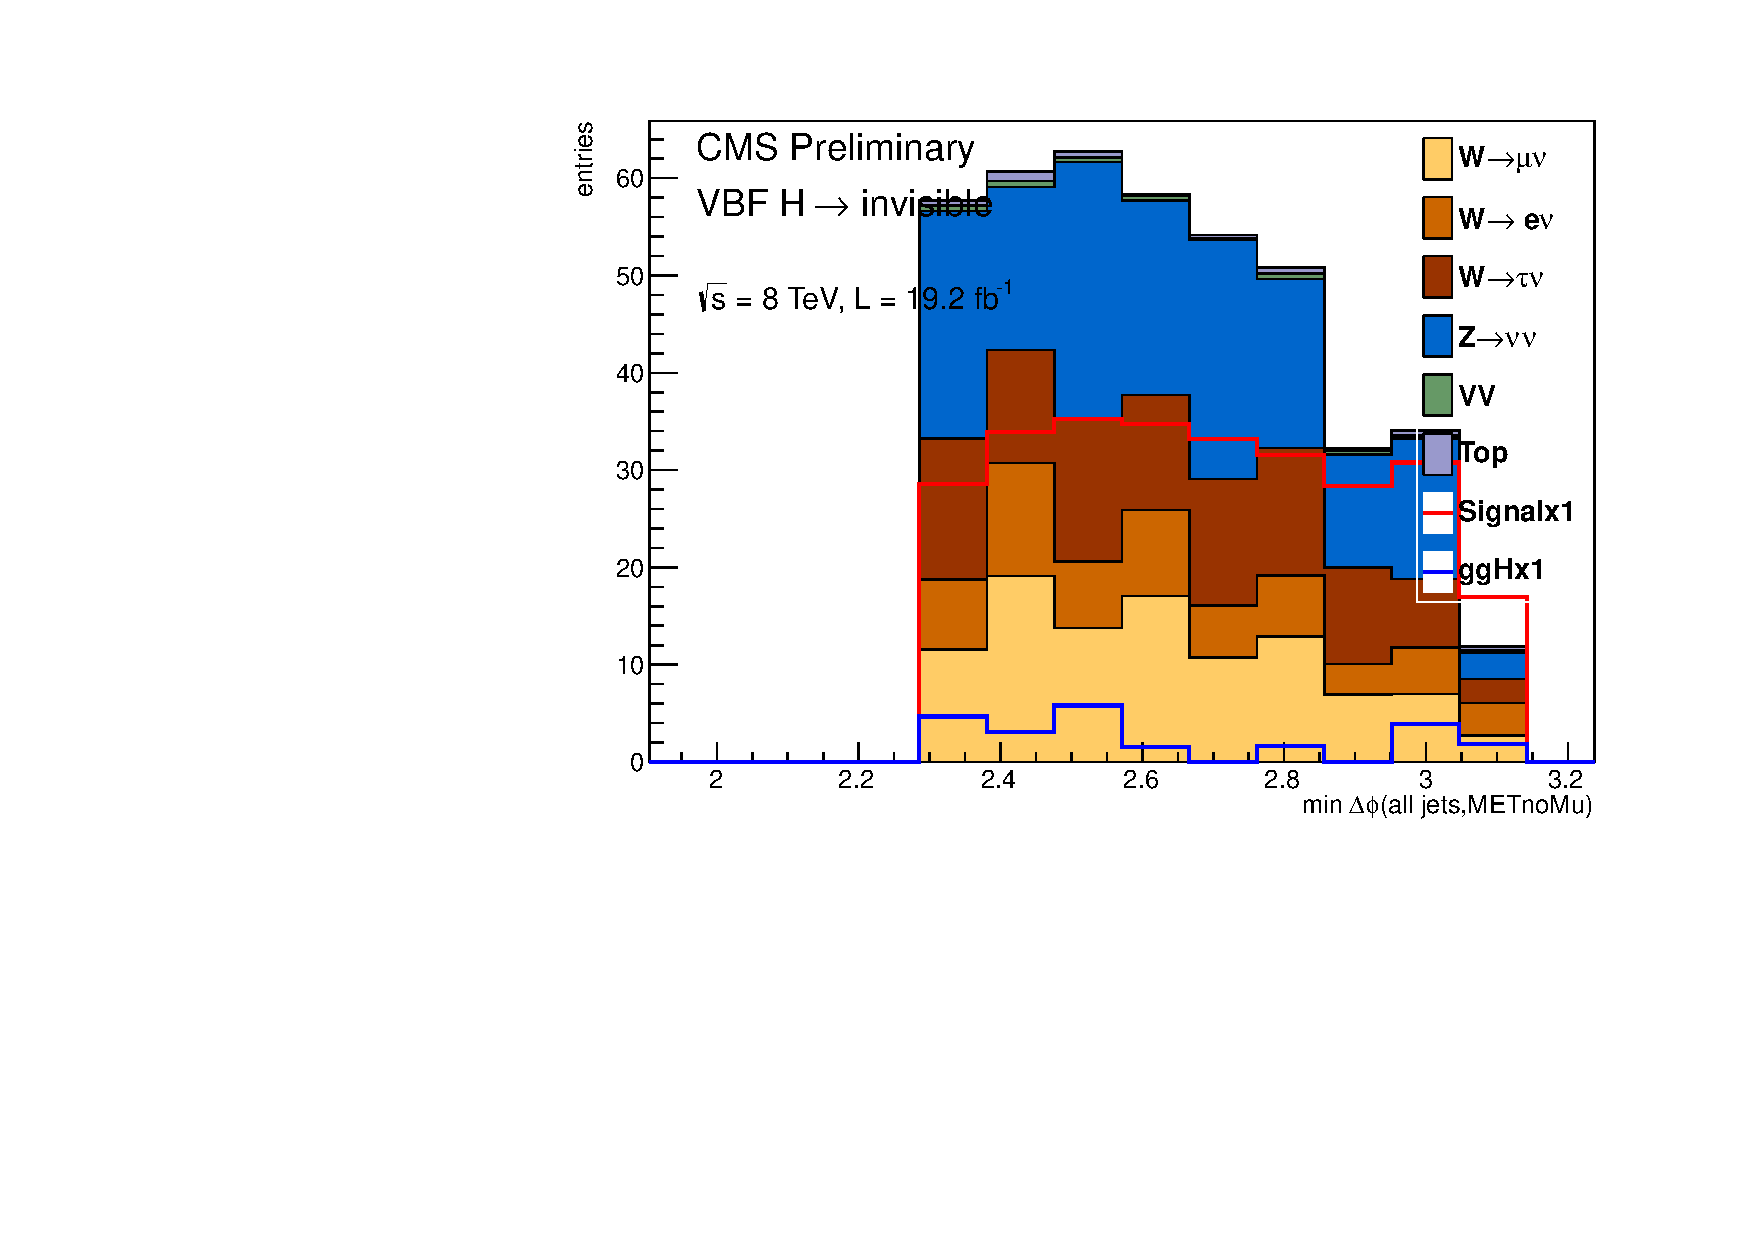
\includegraphics[height=.38\textheight,width=\textwidth]{TalkPics/hig14038preapproval/output_sigreg/nunu_alljetsmetnomu_mindphi.pdf}
    \column{.45\textwidth}
    $METnoMU/\sigma_{METnoMU}$
  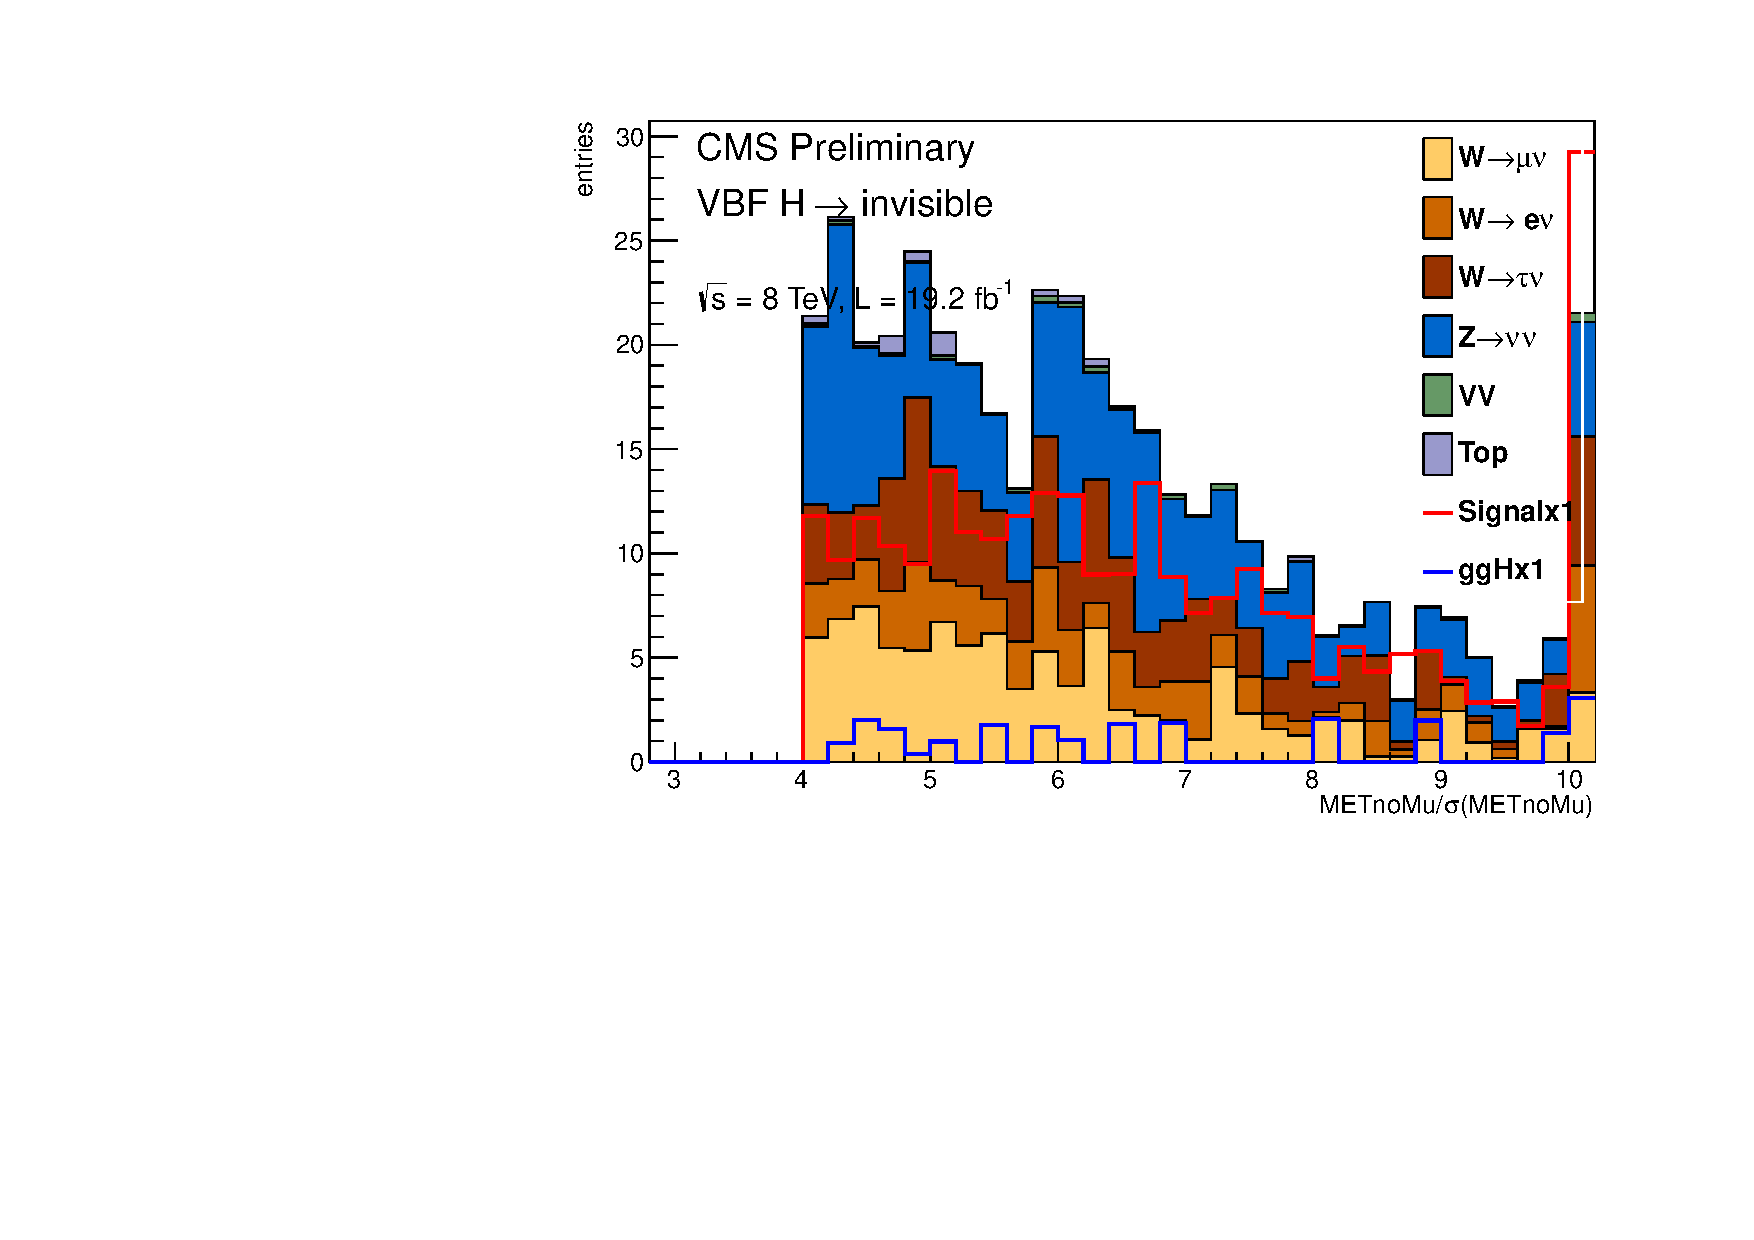
\includegraphics[height=.38\textheight,width=\textwidth]{TalkPics/hig14038preapproval/output_sigreg/nunu_metnomu_significance.pdf}
  \end{columns}
  \begin{columns}
    \column{.45\textwidth}
    \scriptsize
    $Jet 2 p_{T}$
  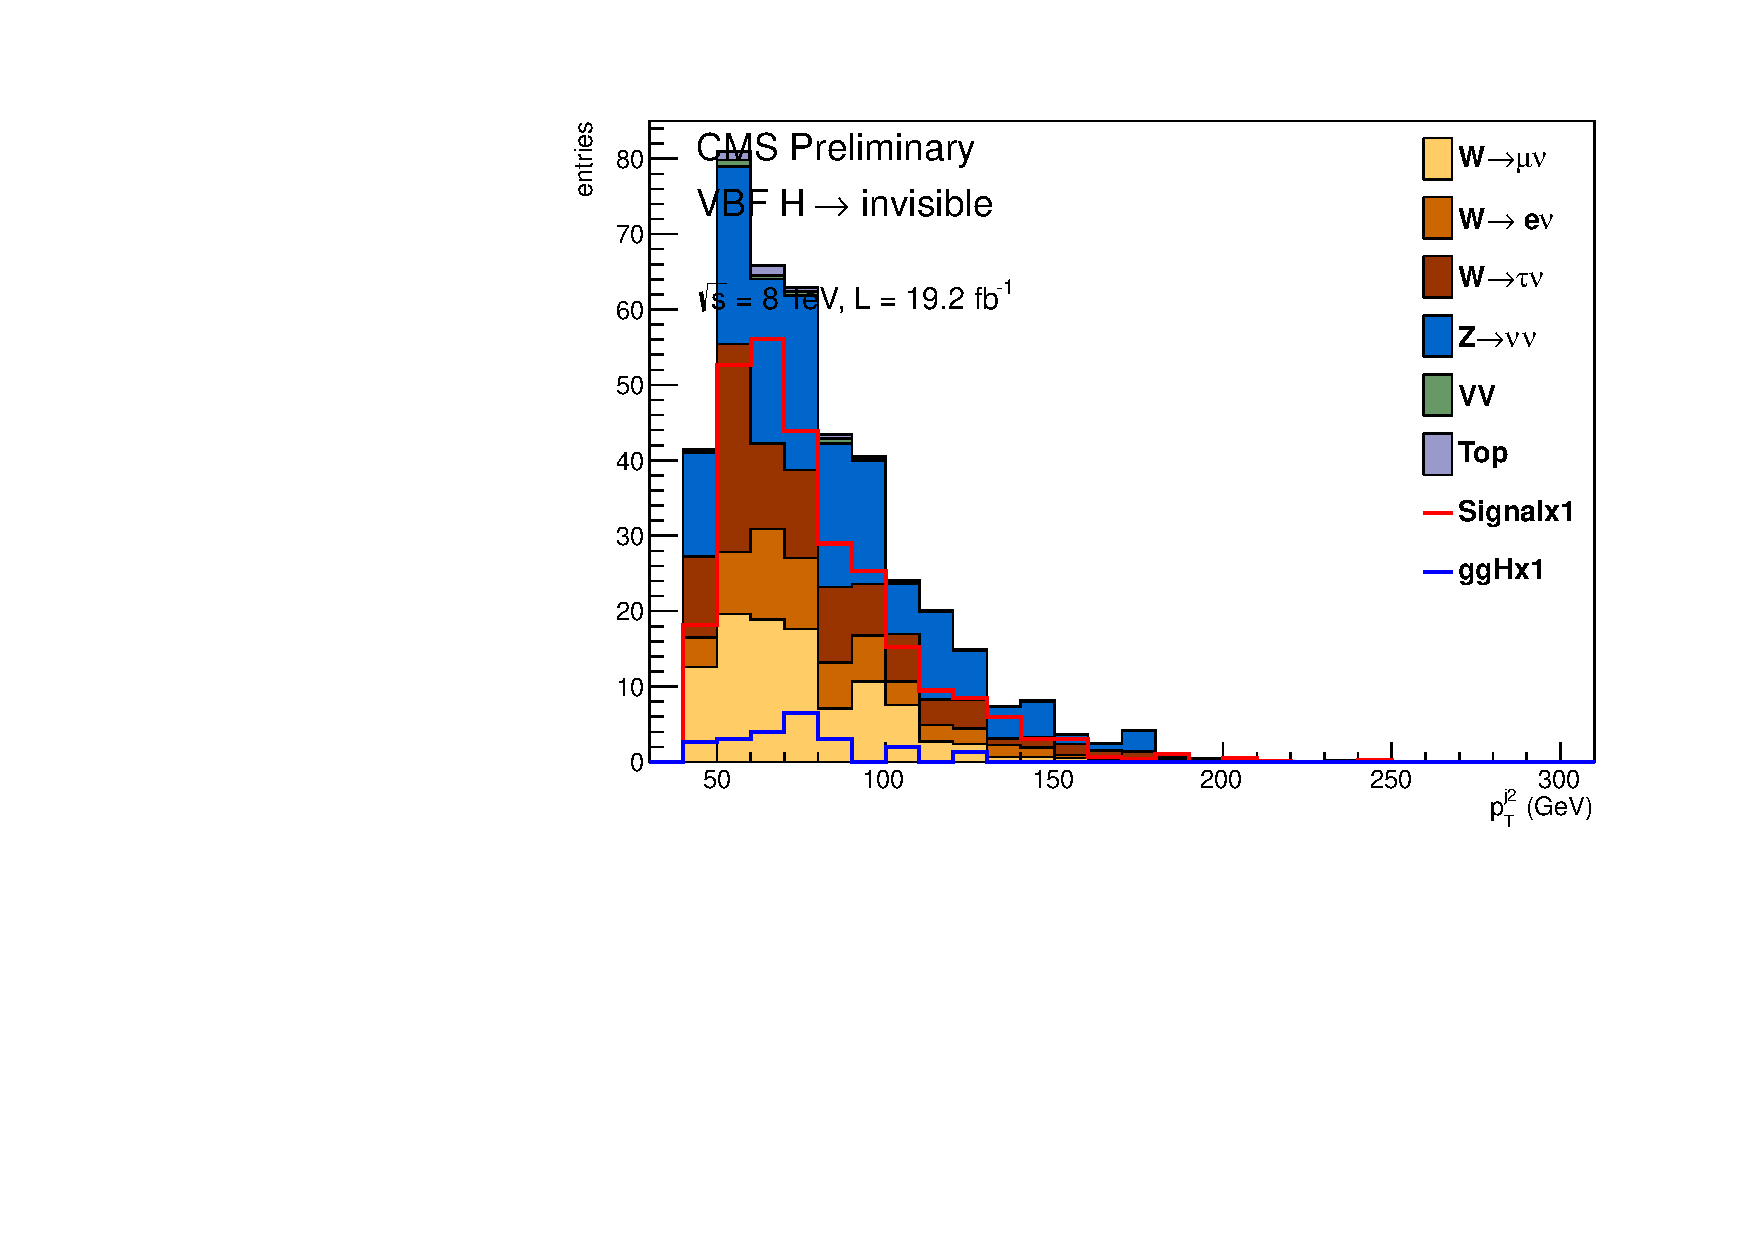
\includegraphics[height=.38\textheight,width=\textwidth]{TalkPics/hig14038preapproval/output_sigreg/nunu_jet2_pt.pdf}
    \column{.45\textwidth}
    $M_{jj}$
  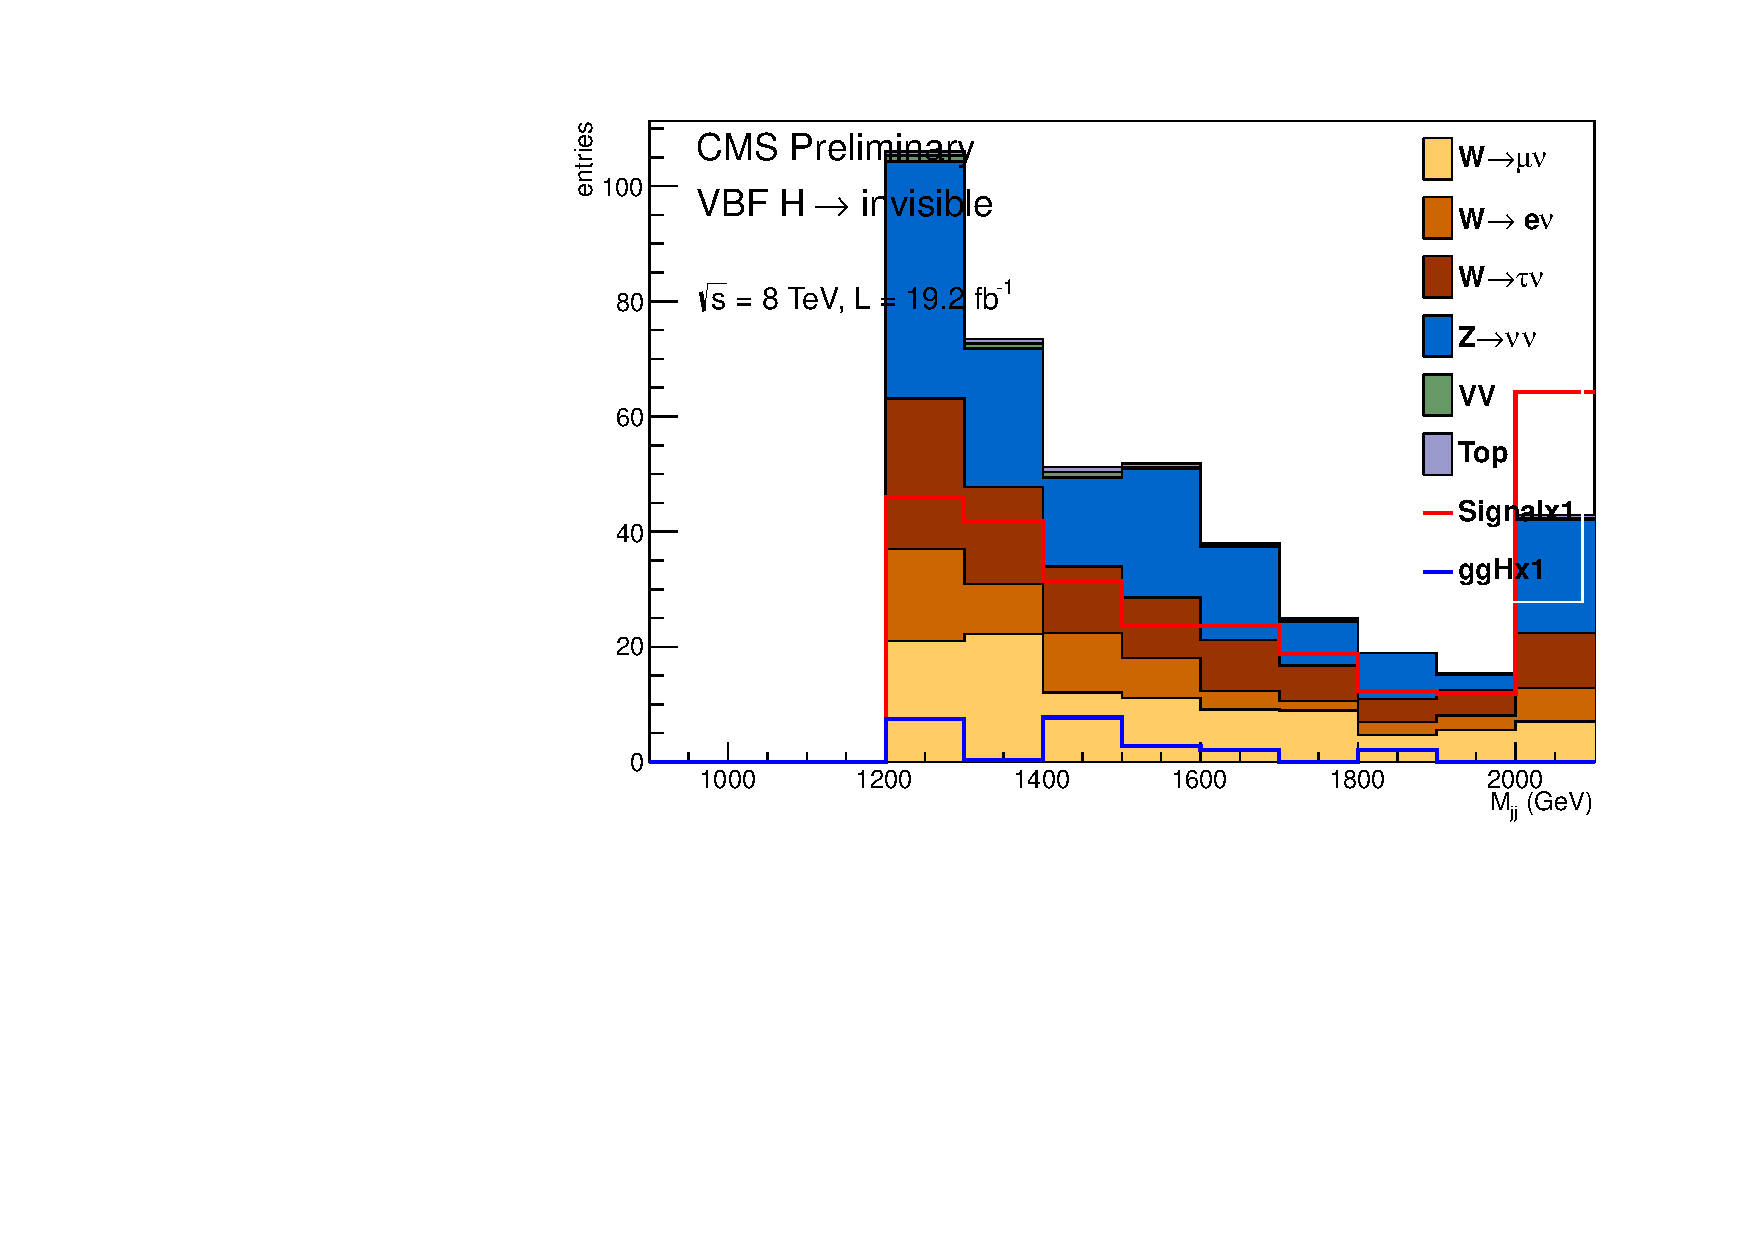
\includegraphics[height=.38\textheight,width=\textwidth]{TalkPics/hig14038preapproval/output_sigreg/nunu_dijet_M.pdf}
  \end{columns}
  \end{block}
\end{frame}



%ADD ALL REMAINING CONTROL PLOTS
\begin{frame}
  \frametitle{Control plots - mumu}
  \begin{columns}
    \column{.5\textwidth}
    \begin{block}{Jet 1 pt}
      \includegraphics[width=\textwidth]{TalkPics/hig14038preapproval/output_sigreg/mumu_jet1_pt.pdf}
    \end{block}
    \column{.5\textwidth}
    \begin{block}{Jet 2 pt}
      \includegraphics[width=\textwidth]{TalkPics/hig14038preapproval/output_sigreg/mumu_jet2_pt.pdf}
    \end{block}

  \end{columns}
\end{frame}

\begin{frame}
  \frametitle{Control plots - mumu}
  \begin{columns}
    \column{.5\textwidth}
    \begin{block}{METnomu}
      \includegraphics[width=\textwidth]{TalkPics/hig14038preapproval/output_sigreg/mumu_metnomuons.pdf}
    \end{block}
    \column{.5\textwidth}
    \begin{block}{METnomusig}
      \includegraphics[width=\textwidth]{TalkPics/hig14038preapproval/output_sigreg/mumu_metnomu_significance.pdf}
    \end{block}

  \end{columns}
\end{frame}

\begin{frame}
  \frametitle{Control plots - mumu }
  \begin{columns}
    \column{.5\textwidth}
    \begin{block}{Mjj}
      \includegraphics[width=\textwidth]{TalkPics/hig14038preapproval/output_sigreg/mumu_dijet_M.pdf}
    \end{block}
    \column{.5\textwidth}
    \begin{block}{dijet-metnomu pt fraction}
      \includegraphics[width=\textwidth]{TalkPics/hig14038preapproval/output_sigreg/mumu_dijetmetnomu_ptfraction.pdf}
    \end{block}
  \end{columns}
\end{frame}

\begin{frame}
  \frametitle{Control plots -mumu}
  \begin{columns}
    \column{.5\textwidth}
    \begin{block}{Dphijj}
      \includegraphics[width=\textwidth]{TalkPics/hig14038preapproval/output_sigreg/mumu_dijet_dphi.pdf}
    \end{block}
    \column{.5\textwidth}
    \begin{block}{Detajj}
      \includegraphics[width=\textwidth]{TalkPics/hig14038preapproval/output_sigreg/mumu_dijet_deta.pdf}
    \end{block}

  \end{columns}
\end{frame}

\begin{frame}
  \frametitle{Control plots -mumu}
  \begin{columns}
    \column{.5\textwidth}
    \begin{block}{Leading jets-met mindphi}
      \includegraphics[width=\textwidth]{TalkPics/hig14038preapproval/output_sigreg/mumu_jetmetnomu_mindphi.pdf}
    \end{block}
    \column{.5\textwidth}
    \begin{block}{All jet-met mindphi}
      \includegraphics[width=\textwidth]{TalkPics/hig14038preapproval/output_sigreg/mumu_alljetsmetnomu_mindphi.pdf}
    \end{block}

  \end{columns}
\end{frame}

\begin{frame}
  \frametitle{Control plots -enu}
  \begin{columns}
    \column{.5\textwidth}
    \begin{block}{Jet 1 pt}
      \includegraphics[width=\textwidth]{TalkPics/hig14038preapproval/output_sigreg/enu_jet1_pt.pdf}
    \end{block}
    \column{.5\textwidth}
    \begin{block}{Jet 2 pt}
      \includegraphics[width=\textwidth]{TalkPics/hig14038preapproval/output_sigreg/enu_jet2_pt.pdf}
    \end{block}

  \end{columns}
\end{frame}

\begin{frame}
  \frametitle{Control plots -enu}
  \begin{columns}
    \column{.5\textwidth}
    \begin{block}{METnomu}
      \includegraphics[width=\textwidth]{TalkPics/hig14038preapproval/output_sigreg/enu_metnomuons.pdf}
    \end{block}
    \column{.5\textwidth}
    \begin{block}{METnomusig}
      \includegraphics[width=\textwidth]{TalkPics/hig14038preapproval/output_sigreg/enu_metnomu_significance.pdf}
    \end{block}

  \end{columns}
\end{frame}

\begin{frame}
  \frametitle{Control plots - enu}
  \begin{columns}
    \column{.5\textwidth}
    \begin{block}{Mjj}
      \includegraphics[width=\textwidth]{TalkPics/hig14038preapproval/output_sigreg/enu_dijet_M.pdf}
    \end{block}
    \column{.5\textwidth}
    \begin{block}{mt}
      \includegraphics[width=\textwidth]{TalkPics/hig14038preapproval/output_sigreg/enu_lep_mt.pdf}
    \end{block}
  \end{columns}
\end{frame}

\begin{frame}
  \frametitle{Control plots - enu}
  \begin{columns}
    \column{.5\textwidth}
    \begin{block}{Dijet Dphi}
      \includegraphics[width=\textwidth]{TalkPics/hig14038preapproval/output_sigreg/enu_dijet_dphi.pdf}
    \end{block}
    \column{.5\textwidth}
    \begin{block}{Detajj}
      \includegraphics[width=\textwidth]{TalkPics/hig14038preapproval/output_sigreg/enu_dijet_deta.pdf}
    \end{block}

  \end{columns}
\end{frame}

\begin{frame}
  \frametitle{Control plots - enu}
  \begin{columns}
    \column{.5\textwidth}
    \begin{block}{Leading jets-met mindphi}
      \includegraphics[width=\textwidth]{TalkPics/hig14038preapproval/output_sigreg/enu_jetmetnomu_mindphi.pdf}
    \end{block}
    \column{.5\textwidth}
    \begin{block}{All jets-met mindphi}
      \includegraphics[width=\textwidth]{TalkPics/hig14038preapproval/output_sigreg/enu_alljetsmetnomu_mindphi.pdf}
    \end{block}

  \end{columns}
\end{frame}

\begin{frame}
  \frametitle{Control plots - enu}
  \begin{columns}
    \column{.5\textwidth}
    \begin{block}{dijet-metnomu pt fraction}
      \includegraphics[width=\textwidth]{TalkPics/hig14038preapproval/output_sigreg/enu_dijetmetnomu_ptfraction.pdf}
    \end{block}
  \end{columns}
\end{frame}

\begin{frame}
  \frametitle{Control plots - munu}
  \begin{columns}
    \column{.5\textwidth}
    \begin{block}{Jet 1 pt}
      \includegraphics[width=\textwidth]{TalkPics/hig14038preapproval/output_sigreg/munu_jet1_pt.pdf}
    \end{block}
    \column{.5\textwidth}
    \begin{block}{Jet 2 pt}
      \includegraphics[width=\textwidth]{TalkPics/hig14038preapproval/output_sigreg/munu_jet2_pt.pdf}
    \end{block}

  \end{columns}
\end{frame}

\begin{frame}
  \frametitle{Control plots - munu}
  \begin{columns}
    \column{.5\textwidth}
    \begin{block}{METnomu}
      \includegraphics[width=\textwidth]{TalkPics/hig14038preapproval/output_sigreg/munu_metnomuons.pdf}
    \end{block}
    \column{.5\textwidth}
    \begin{block}{METnomusig}
      \includegraphics[width=\textwidth]{TalkPics/hig14038preapproval/output_sigreg/munu_metnomu_significance.pdf}
    \end{block}

  \end{columns}
\end{frame}

\begin{frame}
  \frametitle{Control plots - munu}
  \begin{columns}
    \column{.5\textwidth}
    \begin{block}{Mjj}
      \includegraphics[width=\textwidth]{TalkPics/hig14038preapproval/output_sigreg/munu_dijet_M.pdf}
    \end{block}
    \column{.5\textwidth}
    \begin{block}{mt}
      \includegraphics[width=\textwidth]{TalkPics/hig14038preapproval/output_sigreg/munu_lep_mt.pdf}
    \end{block}
  \end{columns}
\end{frame}

\begin{frame}
  \frametitle{Control plots - munu}
  \begin{columns}
    \column{.5\textwidth}
    \begin{block}{Dijet Dphi}
      \includegraphics[width=\textwidth]{TalkPics/hig14038preapproval/output_sigreg/munu_dijet_dphi.pdf}
    \end{block}
    \column{.5\textwidth}
    \begin{block}{Detajj}
      \includegraphics[width=\textwidth]{TalkPics/hig14038preapproval/output_sigreg/munu_dijet_deta.pdf}
    \end{block}

  \end{columns}
\end{frame}

\begin{frame}
  \frametitle{Control plots - munu}
  \begin{columns}
    \column{.5\textwidth}
    \begin{block}{Leading jets-met mindphi}
      \includegraphics[width=\textwidth]{TalkPics/hig14038preapproval/output_sigreg/munu_jetmetnomu_mindphi.pdf}
    \end{block}
    \column{.5\textwidth}
    \begin{block}{All jets-met mindphi}
      \includegraphics[width=\textwidth]{TalkPics/hig14038preapproval/output_sigreg/munu_alljetsmetnomu_mindphi.pdf}
    \end{block}

  \end{columns}
\end{frame}

\begin{frame}
  \frametitle{Control plots - munu}
  \begin{columns}
    \column{.5\textwidth}
    \begin{block}{dijet-metnomu pt fraction}
      \includegraphics[width=\textwidth]{TalkPics/hig14038preapproval/output_sigreg/munu_dijetmetnomu_ptfraction.pdf}
    \end{block}
  \end{columns}
\end{frame}

\begin{frame}
  \frametitle{Control plots - taunu}
  \begin{columns}
    \column{.5\textwidth}
    \begin{block}{Jet 1 pt}
      \includegraphics[width=\textwidth]{TalkPics/hig14038preapproval/output_sigreg/taunu_jet1_pt.pdf}
    \end{block}
    \column{.5\textwidth}
    \begin{block}{Jet 2 pt}
      \includegraphics[width=\textwidth]{TalkPics/hig14038preapproval/output_sigreg/taunu_jet2_pt.pdf}
    \end{block}

  \end{columns}
\end{frame}

\begin{frame}
  \frametitle{Control plots - taunu}
  \begin{columns}
    \column{.5\textwidth}
    \begin{block}{METnomu}
      \includegraphics[width=\textwidth]{TalkPics/hig14038preapproval/output_sigreg/taunu_metnomuons.pdf}
    \end{block}
    \column{.5\textwidth}
    \begin{block}{METnomusig}
      \includegraphics[width=\textwidth]{TalkPics/hig14038preapproval/output_sigreg/taunu_metnomu_significance.pdf}
    \end{block}

  \end{columns}
\end{frame}

\begin{frame}
  \frametitle{Control plots - taunu}
  \begin{columns}
    \column{.5\textwidth}
    \begin{block}{Mjj}
      \includegraphics[width=\textwidth]{TalkPics/hig14038preapproval/output_sigreg/taunu_dijet_M.pdf}
    \end{block}
    \column{.5\textwidth}
    \begin{block}{mt}
      \includegraphics[width=\textwidth]{TalkPics/hig14038preapproval/output_sigreg/taunu_lep_mt.pdf}
    \end{block}
  \end{columns}
\end{frame}

\begin{frame}
  \frametitle{Control plots - taunu}
  \begin{columns}
    \column{.5\textwidth}
    \begin{block}{Dijet Dphi}
      \includegraphics[width=\textwidth]{TalkPics/hig14038preapproval/output_sigreg/taunu_dijet_dphi.pdf}
    \end{block}
    \column{.5\textwidth}
    \begin{block}{Detajj}
      \includegraphics[width=\textwidth]{TalkPics/hig14038preapproval/output_sigreg/taunu_dijet_deta.pdf}
    \end{block}

  \end{columns}
\end{frame}

\begin{frame}
  \frametitle{Control plots - taunu}
  \begin{columns}
    \column{.5\textwidth}
    \begin{block}{Leading jets-met mindphi}
      \includegraphics[width=\textwidth]{TalkPics/hig14038preapproval/output_sigreg/taunu_jetmetnomu_mindphi.pdf}
    \end{block}
    \column{.5\textwidth}
    \begin{block}{All jets-met mindphi}
      \includegraphics[width=\textwidth]{TalkPics/hig14038preapproval/output_sigreg/taunu_alljetsmetnomu_mindphi.pdf}
    \end{block}

  \end{columns}
\end{frame}

\begin{frame}
  \frametitle{Control plots - taunu}
  \begin{columns}
    \column{.5\textwidth}
    \begin{block}{dijet-metnomu pt fraction}
      \includegraphics[width=\textwidth]{TalkPics/hig14038preapproval/output_sigreg/taunu_dijetmetnomu_ptfraction.pdf}
    \end{block}
  \end{columns}
\end{frame}

\begin{frame}
  \frametitle{Control plots - nunu}
  \begin{columns}
    \column{.5\textwidth}
    \begin{block}{Jet 1 pt}
      \includegraphics[width=\textwidth]{TalkPics/hig14038preapproval/output_sigreg/nunu_jet1_pt.pdf}
    \end{block}
    \column{.5\textwidth}
    \begin{block}{Jet 2 pt}
      \includegraphics[width=\textwidth]{TalkPics/hig14038preapproval/output_sigreg/nunu_jet2_pt.pdf}
    \end{block}

  \end{columns}
\end{frame}

\begin{frame}
  \frametitle{Control plots - nunu}
  \begin{columns}
    \column{.5\textwidth}
    \begin{block}{METnomu}
      \includegraphics[width=\textwidth]{TalkPics/hig14038preapproval/output_sigreg/nunu_metnomuons.pdf}
    \end{block}
    \column{.5\textwidth}
    \begin{block}{METnomusig}
      \includegraphics[width=\textwidth]{TalkPics/hig14038preapproval/output_sigreg/nunu_metnomu_significance.pdf}
    \end{block}

  \end{columns}
\end{frame}

\begin{frame}
  \frametitle{Control plots - nunu}
  \begin{columns}
    \column{.5\textwidth}
    \begin{block}{Mjj}
      \includegraphics[width=\textwidth]{TalkPics/hig14038preapproval/output_sigreg/nunu_dijet_M.pdf}
    \end{block}
    \column{.5\textwidth}
  \end{columns}
\end{frame}

\begin{frame}
  \frametitle{Control plots - nunu}
  \begin{columns}
    \column{.5\textwidth}
    \begin{block}{Dijet Dphi}
      \includegraphics[width=\textwidth]{TalkPics/hig14038preapproval/output_sigreg/nunu_dijet_dphi.pdf}
    \end{block}
    \column{.5\textwidth}
    \begin{block}{Detajj}
      \includegraphics[width=\textwidth]{TalkPics/hig14038preapproval/output_sigreg/nunu_dijet_deta.pdf}
    \end{block}

  \end{columns}
\end{frame}

\begin{frame}
  \frametitle{Control plots - nunu}
  \begin{columns}
    \column{.5\textwidth}
    \begin{block}{Leading jets-met mindphi}
      \includegraphics[width=\textwidth]{TalkPics/hig14038preapproval/output_sigreg/nunu_jetmetnomu_mindphi.pdf}
    \end{block}
    \column{.5\textwidth}
    \begin{block}{All jets-met mindphi}
      \includegraphics[width=\textwidth]{TalkPics/hig14038preapproval/output_sigreg/nunu_alljetsmetnomu_mindphi.pdf}
    \end{block}

  \end{columns}
\end{frame}

\begin{frame}
  \frametitle{Control plots - nunu}
  \begin{columns}
    \column{.5\textwidth}
    \begin{block}{dijet-metnomu pt fraction}
      \includegraphics[width=\textwidth]{TalkPics/hig14038preapproval/output_sigreg/nunu_dijetmetnomu_ptfraction.pdf}
    \end{block}
  \end{columns}
\end{frame}

\begin{frame}
  \frametitle{Trigger efficiency error}
  \begin{block}{}
    \begin{itemize}
      \item Bin used with largest uncertainty picked for each run period
      \item Worst case scenario assumed of all bins having this uncertainty gives 2.3\% uncertainty
      \item Error cancels in all data driven backgrounds
      \item Only affects signal and VV
      \item Small compared to other uncertainties and doesn't affect limit
      \item Treated as negligible
    \end{itemize}
  \end{block}
\end{frame}

%ALL TRIGGER EFF PLOTS
\begin{frame}
\frametitle{Trigger efficiency-Run A-1}
  \begin{figure}[h!]
  \begin{center}
    \includegraphics[width=.25\textwidth]{TalkPics/hig14038preapproval/trigfitplots/hData_MET_1D_11A.pdf}
    \includegraphics[width=.25\textwidth]{TalkPics/hig14038preapproval/trigfitplots/hData_MET_1D_12A.pdf}
    \includegraphics[width=.25\textwidth]{TalkPics/hig14038preapproval/trigfitplots/hData_MET_1D_13A.pdf}
    \includegraphics[width=.25\textwidth]{TalkPics/hig14038preapproval/trigfitplots/hData_MET_1D_14A.pdf}

    \includegraphics[width=.25\textwidth]{TalkPics/hig14038preapproval/trigfitplots/hData_MET_1D_15A.pdf}
    \includegraphics[width=.25\textwidth]{TalkPics/hig14038preapproval/trigfitplots/hData_MET_1D_21A.pdf}
    \includegraphics[width=.25\textwidth]{TalkPics/hig14038preapproval/trigfitplots/hData_MET_1D_22A.pdf}
    \includegraphics[width=.25\textwidth]{TalkPics/hig14038preapproval/trigfitplots/hData_MET_1D_23A.pdf}

    \includegraphics[width=.25\textwidth]{TalkPics/hig14038preapproval/trigfitplots/hData_MET_1D_24A.pdf}
    \includegraphics[width=.25\textwidth]{TalkPics/hig14038preapproval/trigfitplots/hData_MET_1D_25A.pdf}

  \end{center}
\end{figure}
\end{frame}
\begin{frame}
\frametitle{Trigger efficiency-Run A-2}
\begin{figure}[h!]
  \begin{center}
    \includegraphics[width=.25\textwidth]{TalkPics/hig14038preapproval/trigfitplots/hData_MET_1D_31A.pdf}
    \includegraphics[width=.25\textwidth]{TalkPics/hig14038preapproval/trigfitplots/hData_MET_1D_32A.pdf}
    \includegraphics[width=.25\textwidth]{TalkPics/hig14038preapproval/trigfitplots/hData_MET_1D_33A.pdf}
    \includegraphics[width=.25\textwidth]{TalkPics/hig14038preapproval/trigfitplots/hData_MET_1D_34A.pdf}

    \includegraphics[width=.25\textwidth]{TalkPics/hig14038preapproval/trigfitplots/hData_MET_1D_35A.pdf}
    \includegraphics[width=.25\textwidth]{TalkPics/hig14038preapproval/trigfitplots/hData_MET_1D_41A.pdf}
    \includegraphics[width=.25\textwidth]{TalkPics/hig14038preapproval/trigfitplots/hData_MET_1D_42A.pdf}
    \includegraphics[width=.25\textwidth]{TalkPics/hig14038preapproval/trigfitplots/hData_MET_1D_43A.pdf}

    \includegraphics[width=.25\textwidth]{TalkPics/hig14038preapproval/trigfitplots/hData_MET_1D_44A.pdf}
    \includegraphics[width=.25\textwidth]{TalkPics/hig14038preapproval/trigfitplots/hData_MET_1D_45A.pdf}
  \end{center}
\end{figure}
\end{frame}

\begin{frame}
\frametitle{Trigger efficiency-Run BC-1}
  \begin{figure}[h!]
  \begin{center}
    \includegraphics[width=.25\textwidth]{TalkPics/hig14038preapproval/trigfitplots/hData_MET_1D_11BC.pdf}
    \includegraphics[width=.25\textwidth]{TalkPics/hig14038preapproval/trigfitplots/hData_MET_1D_12BC.pdf}
    \includegraphics[width=.25\textwidth]{TalkPics/hig14038preapproval/trigfitplots/hData_MET_1D_13BC.pdf}
    \includegraphics[width=.25\textwidth]{TalkPics/hig14038preapproval/trigfitplots/hData_MET_1D_14BC.pdf}

    \includegraphics[width=.25\textwidth]{TalkPics/hig14038preapproval/trigfitplots/hData_MET_1D_15BC.pdf}
    \includegraphics[width=.25\textwidth]{TalkPics/hig14038preapproval/trigfitplots/hData_MET_1D_21BC.pdf}
    \includegraphics[width=.25\textwidth]{TalkPics/hig14038preapproval/trigfitplots/hData_MET_1D_22BC.pdf}
    \includegraphics[width=.25\textwidth]{TalkPics/hig14038preapproval/trigfitplots/hData_MET_1D_23BC.pdf}

    \includegraphics[width=.25\textwidth]{TalkPics/hig14038preapproval/trigfitplots/hData_MET_1D_24BC.pdf}
    \includegraphics[width=.25\textwidth]{TalkPics/hig14038preapproval/trigfitplots/hData_MET_1D_25BC.pdf}

  \end{center}
\end{figure}
\end{frame}
\begin{frame}
\frametitle{Trigger efficiency-Run BC-2}
\begin{figure}[h!]
  \begin{center}
    \includegraphics[width=.25\textwidth]{TalkPics/hig14038preapproval/trigfitplots/hData_MET_1D_31BC.pdf}
    \includegraphics[width=.25\textwidth]{TalkPics/hig14038preapproval/trigfitplots/hData_MET_1D_32BC.pdf}
    \includegraphics[width=.25\textwidth]{TalkPics/hig14038preapproval/trigfitplots/hData_MET_1D_33BC.pdf}
    \includegraphics[width=.25\textwidth]{TalkPics/hig14038preapproval/trigfitplots/hData_MET_1D_34BC.pdf}

    \includegraphics[width=.25\textwidth]{TalkPics/hig14038preapproval/trigfitplots/hData_MET_1D_35BC.pdf}
    \includegraphics[width=.25\textwidth]{TalkPics/hig14038preapproval/trigfitplots/hData_MET_1D_41BC.pdf}
    \includegraphics[width=.25\textwidth]{TalkPics/hig14038preapproval/trigfitplots/hData_MET_1D_42BC.pdf}
    \includegraphics[width=.25\textwidth]{TalkPics/hig14038preapproval/trigfitplots/hData_MET_1D_43BC.pdf}

    \includegraphics[width=.25\textwidth]{TalkPics/hig14038preapproval/trigfitplots/hData_MET_1D_44BC.pdf}
    \includegraphics[width=.25\textwidth]{TalkPics/hig14038preapproval/trigfitplots/hData_MET_1D_45BC.pdf}
  \end{center}
\end{figure}
\end{frame}

\begin{frame}
\frametitle{Trigger efficiency-Run D-1}
  \begin{figure}[h!]
  \begin{center}
    \includegraphics[width=.25\textwidth]{TalkPics/hig14038preapproval/trigfitplots/hData_MET_1D_11D.pdf}
    \includegraphics[width=.25\textwidth]{TalkPics/hig14038preapproval/trigfitplots/hData_MET_1D_12D.pdf}
    \includegraphics[width=.25\textwidth]{TalkPics/hig14038preapproval/trigfitplots/hData_MET_1D_13D.pdf}
    \includegraphics[width=.25\textwidth]{TalkPics/hig14038preapproval/trigfitplots/hData_MET_1D_14D.pdf}

    \includegraphics[width=.25\textwidth]{TalkPics/hig14038preapproval/trigfitplots/hData_MET_1D_15D.pdf}
    \includegraphics[width=.25\textwidth]{TalkPics/hig14038preapproval/trigfitplots/hData_MET_1D_21D.pdf}
    \includegraphics[width=.25\textwidth]{TalkPics/hig14038preapproval/trigfitplots/hData_MET_1D_22D.pdf}
    \includegraphics[width=.25\textwidth]{TalkPics/hig14038preapproval/trigfitplots/hData_MET_1D_23D.pdf}

    \includegraphics[width=.25\textwidth]{TalkPics/hig14038preapproval/trigfitplots/hData_MET_1D_24D.pdf}
    \includegraphics[width=.25\textwidth]{TalkPics/hig14038preapproval/trigfitplots/hData_MET_1D_25D.pdf}

  \end{center}
\end{figure}
\end{frame}
\begin{frame}
\frametitle{Trigger efficiency-Run D-2}
\begin{figure}[h!]
  \begin{center}
    \includegraphics[width=.25\textwidth]{TalkPics/hig14038preapproval/trigfitplots/hData_MET_1D_31D.pdf}
    \includegraphics[width=.25\textwidth]{TalkPics/hig14038preapproval/trigfitplots/hData_MET_1D_32D.pdf}
    \includegraphics[width=.25\textwidth]{TalkPics/hig14038preapproval/trigfitplots/hData_MET_1D_33D.pdf}
    \includegraphics[width=.25\textwidth]{TalkPics/hig14038preapproval/trigfitplots/hData_MET_1D_34D.pdf}

    \includegraphics[width=.25\textwidth]{TalkPics/hig14038preapproval/trigfitplots/hData_MET_1D_35D.pdf}
    \includegraphics[width=.25\textwidth]{TalkPics/hig14038preapproval/trigfitplots/hData_MET_1D_41D.pdf}
    \includegraphics[width=.25\textwidth]{TalkPics/hig14038preapproval/trigfitplots/hData_MET_1D_42D.pdf}
    \includegraphics[width=.25\textwidth]{TalkPics/hig14038preapproval/trigfitplots/hData_MET_1D_43D.pdf}

    \includegraphics[width=.25\textwidth]{TalkPics/hig14038preapproval/trigfitplots/hData_MET_1D_44D.pdf}
    \includegraphics[width=.25\textwidth]{TalkPics/hig14038preapproval/trigfitplots/hData_MET_1D_45D.pdf}
  \end{center}
\end{figure}
\end{frame}





\begin{frame}
  \frametitle{QCD options tried}
  \begin{block}{}
    \scriptsize Several methods tried to model QCD
  \end{block}
  \begin{block}{\scriptsize Standard MC}
    \scriptsize
    \begin{itemize}
    \item[-] doesn't have enough events
    \end{itemize}
  \end{block}
  \begin{block}{\scriptsize Private VBF$+$MET enriched QCD MC sample}
    \scriptsize
    \begin{itemize}
    \item[-] Can only enrich in events with real met
    \item[-] Can't model met from mismeasurement
    \end{itemize}
  \end{block}
  \begin{block}{\scriptsize Data-driven shape using different jet pairs in the event}
    \scriptsize
    \begin{itemize}
    \item[-] Jet kinematics are very biased
    \item[-] Ordering in $p_{T}$ and angle have been tried
    \item[-] Reweighting individual distributions to fix others has been tried
    \end{itemize}
  \end{block}
\end{frame}

\begin{frame}{VBF enriched QCD MC}
  \vspace{-.3cm}

  \begin{columns}
    \column{0.45\linewidth} 
    \begin{block}{\begin{tiny}MC Filter: Vectorial sum of neutrino $E_T$\end{tiny}}
      \begin{itemize}
      \item $\sum E_\perp(\vec{\nu}) > 40$ $GeV$
      \end{itemize}
    \end{block}
    \vspace{-.3cm}
    \begin{block}{\begin{tiny}MC Filter: Dijet Filter\end{tiny}}
      \tiny
      \begin{itemize}
      \item Select jets with:
        \begin{itemize}
          \scriptsize
        \item $p_\perp>20$ $GeV$
        \item $|\eta|<5.0$
        \end{itemize}
      \item From selected jets at least one pair with:
        \begin{itemize}
          \scriptsize
        \item $m_{jj}>700$ $GeV$
        \item $\Delta\eta>3.2$
        \end{itemize}  
      \end{itemize}
    \end{block}
    \column{0.45\linewidth} 
    \begin{block}{\tiny QCD Inc 80-600 $GeV$}
      \tiny
      \centering
      \includegraphics[width=0.7\linewidth]{TalkPics/higgsexo031114/MC_QCDIncAll_GenVsReco_met}

      There 2 distict populations of events: real and fake met.
    \end{block}
\end{columns}
  \vspace{-.1cm}

\begin{block}
  \scriptsize
  \centering
  \resizebox{0.8\linewidth}{!}{
    \begin{tabular}{|c|r|c|r|c|c|}
      \hline
      Sample          &       Ev. Gen. & Filter Eff. &  Events &  XS $[pb]$ & Eq. Lumi. $[fb^{-1}]$ \\
      \hline \hline
      QCD-Pt-80to120  & 39376000000 &    0.000049 & 1614416 &  1033680 &  38.09 \\
      QCD-Pt-120to170 &  7000000000 &    0.000283 & 2051000 & 156293.3 &  44.79 \\
      QCD-Pt-170to300 &  1375000000 &    0.000987 & 1391500 & 34138.15 &  40.28 \\
      QCD-Pt-300to470 &    80000000 &    0.002659 &  207840 & 1759.549 &  45.47 \\
      QCD-Pt-470to600 &    25000000 &    0.004127 &  104675 & 113.8791 & 219.53 \\
      \hline
    \end{tabular}
  }
\end{block}

\end{frame}

%BDT FIRST LOOK  WITH CAVEATS
\begin{frame}
  \frametitle{BDT Study}
  \begin{columns}
    \column{.55\textwidth}
    \begin{block}{}
      \scriptsize
      \begin{itemize}
      \item Had a quick look at MVA analysis
      \item Started from cut based signal region
      \item[-] Only region with negligible QCD
      \item Best expected limit obtained 37\%
      \item[-] Does not take into account any increased systematic
      \item[-] Therefore unlikely to be worthwhile
      \item New variables could make MVA worthwile
      \item Ability to model QCD would enable looser starting selection which may make MVA worthwhile
      \end{itemize}
    \end{block}
    \column{.5\textwidth}
    \includegraphics[width=\textwidth]{TalkPics/hig14038preapproval/fishersoverb.pdf}
  \end{columns}
\end{frame}

\begin{frame}
  \frametitle{MVA Details}
  \centering
  \includegraphics[width=.75\textwidth]{TalkPics/hig14038preapproval/mvainputs1.pdf}

  \includegraphics[clip=true,trim=0 140 0 0 ,width=.75\textwidth]{TalkPics/hig14038preapproval/mvainputs2.pdf} 
\end{frame}

\begin{frame}
  \frametitle{MVA Details}
  \includegraphics[width=.49\textwidth]{TalkPics/hig14038preapproval/inputcorrsig.pdf}
  \hspace{.1cm}
  \includegraphics[width=.49\textwidth]{TalkPics/hig14038preapproval/inputcorrbkg.pdf}
\end{frame}

\begin{frame}
  \frametitle{MVA Details}
  \includegraphics[width=.49\textwidth]{TalkPics/hig14038preapproval/fisherdist.pdf}
  \hspace{.1cm}
  \includegraphics[width=.49\textwidth]{TalkPics/hig14038preapproval/bdtdist.pdf}
\end{frame}

\begin{frame}
  \frametitle{MVA Details}
  \includegraphics[width=.49\textwidth]{TalkPics/hig14038preapproval/fishersoverb.pdf}
  \hspace{.1cm}
  \includegraphics[width=.49\textwidth]{TalkPics/hig14038preapproval/bdtsoverb.pdf} 
\end{frame}


\begin{frame}
  \frametitle{No systematics limits}
  \begin{block}{}
    \begin{itemize}
    \item Prompt limit with no systematics 16.6\%
    \item Parked limit with no systematics 14.3\%
    \end{itemize}
  \end{block}
\end{frame}



\end{fmffile}
\end{document}
